\documentclass[twoside]{book}

% Packages required by doxygen
\usepackage{fixltx2e}
\usepackage{calc}
\usepackage{doxygen}
\usepackage[export]{adjustbox} % also loads graphicx
\usepackage{graphicx}
\usepackage[utf8]{inputenc}
\usepackage{makeidx}
\usepackage{multicol}
\usepackage{multirow}
\PassOptionsToPackage{warn}{textcomp}
\usepackage{textcomp}
\usepackage[nointegrals]{wasysym}
\usepackage[table]{xcolor}

% Font selection
\usepackage[T1]{fontenc}
\usepackage[scaled=.90]{helvet}
\usepackage{courier}
\usepackage{amssymb}
\usepackage{sectsty}
\renewcommand{\familydefault}{\sfdefault}
\allsectionsfont{%
  \fontseries{bc}\selectfont%
  \color{darkgray}%
}
\renewcommand{\DoxyLabelFont}{%
  \fontseries{bc}\selectfont%
  \color{darkgray}%
}
\newcommand{\+}{\discretionary{\mbox{\scriptsize$\hookleftarrow$}}{}{}}

% Page & text layout
\usepackage{geometry}
\geometry{%
  a4paper,%
  top=2.5cm,%
  bottom=2.5cm,%
  left=2.5cm,%
  right=2.5cm%
}
\tolerance=750
\hfuzz=15pt
\hbadness=750
\setlength{\emergencystretch}{15pt}
\setlength{\parindent}{0cm}
\setlength{\parskip}{3ex plus 2ex minus 2ex}
\makeatletter
\renewcommand{\paragraph}{%
  \@startsection{paragraph}{4}{0ex}{-1.0ex}{1.0ex}{%
    \normalfont\normalsize\bfseries\SS@parafont%
  }%
}
\renewcommand{\subparagraph}{%
  \@startsection{subparagraph}{5}{0ex}{-1.0ex}{1.0ex}{%
    \normalfont\normalsize\bfseries\SS@subparafont%
  }%
}
\makeatother

% Headers & footers
\usepackage{fancyhdr}
\pagestyle{fancyplain}
\fancyhead[LE]{\fancyplain{}{\bfseries\thepage}}
\fancyhead[CE]{\fancyplain{}{}}
\fancyhead[RE]{\fancyplain{}{\bfseries\leftmark}}
\fancyhead[LO]{\fancyplain{}{\bfseries\rightmark}}
\fancyhead[CO]{\fancyplain{}{}}
\fancyhead[RO]{\fancyplain{}{\bfseries\thepage}}
\fancyfoot[LE]{\fancyplain{}{}}
\fancyfoot[CE]{\fancyplain{}{}}
\fancyfoot[RE]{\fancyplain{}{\bfseries\scriptsize Generated by Doxygen }}
\fancyfoot[LO]{\fancyplain{}{\bfseries\scriptsize Generated by Doxygen }}
\fancyfoot[CO]{\fancyplain{}{}}
\fancyfoot[RO]{\fancyplain{}{}}
\renewcommand{\footrulewidth}{0.4pt}
\renewcommand{\chaptermark}[1]{%
  \markboth{#1}{}%
}
\renewcommand{\sectionmark}[1]{%
  \markright{\thesection\ #1}%
}

% Indices & bibliography
\usepackage{natbib}
\usepackage[titles]{tocloft}
\setcounter{tocdepth}{3}
\setcounter{secnumdepth}{5}
\makeindex

% Hyperlinks (required, but should be loaded last)
\usepackage{ifpdf}
\ifpdf
  \usepackage[pdftex,pagebackref=true]{hyperref}
\else
  \usepackage[ps2pdf,pagebackref=true]{hyperref}
\fi
\hypersetup{%
  colorlinks=true,%
  linkcolor=blue,%
  citecolor=blue,%
  unicode%
}

% Custom commands
\newcommand{\clearemptydoublepage}{%
  \newpage{\pagestyle{empty}\cleardoublepage}%
}

\usepackage{caption}
\captionsetup{labelsep=space,justification=centering,font={bf},singlelinecheck=off,skip=4pt,position=top}

%===== C O N T E N T S =====

\begin{document}

% Titlepage & ToC
\hypersetup{pageanchor=false,
             bookmarksnumbered=true,
             pdfencoding=unicode
            }
\pagenumbering{alph}
\begin{titlepage}
\vspace*{7cm}
\begin{center}%
{\Large Space Invader }\\
\vspace*{1cm}
{\large Generated by Doxygen 1.8.13}\\
\end{center}
\end{titlepage}
\clearemptydoublepage
\pagenumbering{roman}
\tableofcontents
\clearemptydoublepage
\pagenumbering{arabic}
\hypersetup{pageanchor=true}

%--- Begin generated contents ---
\chapter{Namespace Index}
\section{Namespace List}
Here is a list of all documented namespaces with brief descriptions\+:\begin{DoxyCompactList}
\item\contentsline{section}{\hyperlink{namespacegame}{game} }{\pageref{namespacegame}}{}
\end{DoxyCompactList}

\chapter{Hierarchical Index}
\section{Class Hierarchy}
This inheritance list is sorted roughly, but not completely, alphabetically\+:\begin{DoxyCompactList}
\item \contentsline{section}{game\+:\+:Alien\+Builder}{\pageref{classgame_1_1AlienBuilder}}{}
\item \contentsline{section}{Background}{\pageref{classBackground}}{}
\item \contentsline{section}{game\+:\+:Barrier\+Block}{\pageref{classgame_1_1BarrierBlock}}{}
\item \contentsline{section}{game\+:\+:Base}{\pageref{classgame_1_1Base}}{}
\begin{DoxyCompactList}
\item \contentsline{section}{game\+:\+:Alien\+Base}{\pageref{classgame_1_1AlienBase}}{}
\begin{DoxyCompactList}
\item \contentsline{section}{game\+:\+:Alien}{\pageref{classgame_1_1Alien}}{}
\begin{DoxyCompactList}
\item \contentsline{section}{game\+:\+:Hunter}{\pageref{classgame_1_1Hunter}}{}
\end{DoxyCompactList}
\item \contentsline{section}{game\+:\+:Swarm}{\pageref{classgame_1_1Swarm}}{}
\end{DoxyCompactList}
\item \contentsline{section}{game\+:\+:Bullet}{\pageref{classgame_1_1Bullet}}{}
\begin{DoxyCompactList}
\item \contentsline{section}{game\+:\+:Diagonal\+Bullet}{\pageref{classgame_1_1DiagonalBullet}}{}
\end{DoxyCompactList}
\item \contentsline{section}{game\+:\+:Ship}{\pageref{classgame_1_1Ship}}{}
\end{DoxyCompactList}
\item \contentsline{section}{game\+:\+:Bullet\+Builder\+Interface}{\pageref{classgame_1_1BulletBuilderInterface}}{}
\begin{DoxyCompactList}
\item \contentsline{section}{game\+:\+:Bullet\+Builder}{\pageref{classgame_1_1BulletBuilder}}{}
\end{DoxyCompactList}
\item \contentsline{section}{game\+:\+:Command}{\pageref{classgame_1_1Command}}{}
\begin{DoxyCompactList}
\item \contentsline{section}{game\+:\+:Command\+Clear\+Stage}{\pageref{classgame_1_1CommandClearStage}}{}
\item \contentsline{section}{game\+:\+:Command\+Game\+Pause}{\pageref{classgame_1_1CommandGamePause}}{}
\item \contentsline{section}{game\+:\+:Command\+Game\+Start}{\pageref{classgame_1_1CommandGameStart}}{}
\item \contentsline{section}{game\+:\+:Command\+Goto\+Game\+Mode}{\pageref{classgame_1_1CommandGotoGameMode}}{}
\item \contentsline{section}{game\+:\+:Command\+Goto\+Leader\+Board\+Mode}{\pageref{classgame_1_1CommandGotoLeaderBoardMode}}{}
\item \contentsline{section}{game\+:\+:Command\+Goto\+Stage\+Maker\+Mode}{\pageref{classgame_1_1CommandGotoStageMakerMode}}{}
\item \contentsline{section}{game\+:\+:Command\+Goto\+Title\+Screen\+Mode}{\pageref{classgame_1_1CommandGotoTitleScreenMode}}{}
\item \contentsline{section}{game\+:\+:Command\+Restart\+Stage}{\pageref{classgame_1_1CommandRestartStage}}{}
\end{DoxyCompactList}
\item \contentsline{section}{game\+:\+:Config}{\pageref{classgame_1_1Config}}{}
\item \contentsline{section}{game\+:\+:Cursor}{\pageref{classgame_1_1Cursor}}{}
\item \contentsline{section}{game\+:\+:Cursor\+State}{\pageref{classgame_1_1CursorState}}{}
\begin{DoxyCompactList}
\item \contentsline{section}{game\+:\+:Fighter\+State}{\pageref{classgame_1_1FighterState}}{}
\item \contentsline{section}{game\+:\+:Maker\+State}{\pageref{classgame_1_1MakerState}}{}
\item \contentsline{section}{game\+:\+:Normal\+State}{\pageref{classgame_1_1NormalState}}{}
\item \contentsline{section}{game\+:\+:Pen\+State}{\pageref{classgame_1_1PenState}}{}
\end{DoxyCompactList}
\item \contentsline{section}{Explosion}{\pageref{classExplosion}}{}
\item \contentsline{section}{game\+:\+:Laser\+Beam}{\pageref{structgame_1_1LaserBeam}}{}
\item \contentsline{section}{game\+:\+:Leader\+Board}{\pageref{classgame_1_1LeaderBoard}}{}
\item \contentsline{section}{game\+:\+:Menu}{\pageref{classgame_1_1Menu}}{}
\item \contentsline{section}{game\+:\+:Powerup}{\pageref{classgame_1_1Powerup}}{}
\item Q\+Dialog\begin{DoxyCompactList}
\item \contentsline{section}{Dialog}{\pageref{classDialog}}{}
\item \contentsline{section}{game\+:\+:Game\+Dialog}{\pageref{classgame_1_1GameDialog}}{}
\item \contentsline{section}{game\+:\+:Game\+Menu}{\pageref{classgame_1_1GameMenu}}{}
\item \contentsline{section}{game\+:\+:Instruction\+Request}{\pageref{classgame_1_1InstructionRequest}}{}
\item \contentsline{section}{Leader\+Board\+Name\+Request}{\pageref{classLeaderBoardNameRequest}}{}
\end{DoxyCompactList}
\item Q\+Object\begin{DoxyCompactList}
\item \contentsline{section}{game\+:\+:Unit\+Test\+Space\+Invader}{\pageref{classgame_1_1UnitTestSpaceInvader}}{}
\end{DoxyCompactList}
\item \contentsline{section}{game\+:\+:S\+Maker\+Placed\+Object}{\pageref{structgame_1_1SMakerPlacedObject}}{}
\item \contentsline{section}{game\+:\+:Stage\+Maker}{\pageref{classgame_1_1StageMaker}}{}
\item \contentsline{section}{star}{\pageref{structstar}}{}
\item \contentsline{section}{game\+:\+:Status\+Bar}{\pageref{classgame_1_1StatusBar}}{}
\item \contentsline{section}{game\+:\+:Swarm\+Info}{\pageref{classgame_1_1SwarmInfo}}{}
\end{DoxyCompactList}

\chapter{Class Index}
\section{Class List}
Here are the classes, structs, unions and interfaces with brief descriptions\+:\begin{DoxyCompactList}
\item\contentsline{section}{\hyperlink{classgame_1_1Alien}{game\+::\+Alien} }{\pageref{classgame_1_1Alien}}{}
\item\contentsline{section}{\hyperlink{classgame_1_1AlienBase}{game\+::\+Alien\+Base} }{\pageref{classgame_1_1AlienBase}}{}
\item\contentsline{section}{\hyperlink{classgame_1_1AlienBuilder}{game\+::\+Alien\+Builder} }{\pageref{classgame_1_1AlienBuilder}}{}
\item\contentsline{section}{\hyperlink{classBackground}{Background} }{\pageref{classBackground}}{}
\item\contentsline{section}{\hyperlink{classgame_1_1BarrierBlock}{game\+::\+Barrier\+Block} }{\pageref{classgame_1_1BarrierBlock}}{}
\item\contentsline{section}{\hyperlink{classgame_1_1Base}{game\+::\+Base} }{\pageref{classgame_1_1Base}}{}
\item\contentsline{section}{\hyperlink{classgame_1_1Bullet}{game\+::\+Bullet} }{\pageref{classgame_1_1Bullet}}{}
\item\contentsline{section}{\hyperlink{classgame_1_1BulletBuilder}{game\+::\+Bullet\+Builder} }{\pageref{classgame_1_1BulletBuilder}}{}
\item\contentsline{section}{\hyperlink{classgame_1_1BulletBuilderInterface}{game\+::\+Bullet\+Builder\+Interface} }{\pageref{classgame_1_1BulletBuilderInterface}}{}
\item\contentsline{section}{\hyperlink{classgame_1_1Command}{game\+::\+Command} }{\pageref{classgame_1_1Command}}{}
\item\contentsline{section}{\hyperlink{classgame_1_1CommandClearStage}{game\+::\+Command\+Clear\+Stage} }{\pageref{classgame_1_1CommandClearStage}}{}
\item\contentsline{section}{\hyperlink{classgame_1_1CommandGamePause}{game\+::\+Command\+Game\+Pause} }{\pageref{classgame_1_1CommandGamePause}}{}
\item\contentsline{section}{\hyperlink{classgame_1_1CommandGameStart}{game\+::\+Command\+Game\+Start} }{\pageref{classgame_1_1CommandGameStart}}{}
\item\contentsline{section}{\hyperlink{classgame_1_1CommandGotoGameMode}{game\+::\+Command\+Goto\+Game\+Mode} }{\pageref{classgame_1_1CommandGotoGameMode}}{}
\item\contentsline{section}{\hyperlink{classgame_1_1CommandGotoLeaderBoardMode}{game\+::\+Command\+Goto\+Leader\+Board\+Mode} }{\pageref{classgame_1_1CommandGotoLeaderBoardMode}}{}
\item\contentsline{section}{\hyperlink{classgame_1_1CommandGotoStageMakerMode}{game\+::\+Command\+Goto\+Stage\+Maker\+Mode} }{\pageref{classgame_1_1CommandGotoStageMakerMode}}{}
\item\contentsline{section}{\hyperlink{classgame_1_1CommandGotoTitleScreenMode}{game\+::\+Command\+Goto\+Title\+Screen\+Mode} }{\pageref{classgame_1_1CommandGotoTitleScreenMode}}{}
\item\contentsline{section}{\hyperlink{classgame_1_1CommandRestartStage}{game\+::\+Command\+Restart\+Stage} }{\pageref{classgame_1_1CommandRestartStage}}{}
\item\contentsline{section}{\hyperlink{classgame_1_1Config}{game\+::\+Config} }{\pageref{classgame_1_1Config}}{}
\item\contentsline{section}{\hyperlink{classgame_1_1Cursor}{game\+::\+Cursor} }{\pageref{classgame_1_1Cursor}}{}
\item\contentsline{section}{\hyperlink{classgame_1_1CursorState}{game\+::\+Cursor\+State} }{\pageref{classgame_1_1CursorState}}{}
\item\contentsline{section}{\hyperlink{classgame_1_1DiagonalBullet}{game\+::\+Diagonal\+Bullet} }{\pageref{classgame_1_1DiagonalBullet}}{}
\item\contentsline{section}{\hyperlink{classDialog}{Dialog} }{\pageref{classDialog}}{}
\item\contentsline{section}{\hyperlink{classExplosion}{Explosion} }{\pageref{classExplosion}}{}
\item\contentsline{section}{\hyperlink{classgame_1_1FighterState}{game\+::\+Fighter\+State} }{\pageref{classgame_1_1FighterState}}{}
\item\contentsline{section}{\hyperlink{classgame_1_1GameDialog}{game\+::\+Game\+Dialog} }{\pageref{classgame_1_1GameDialog}}{}
\item\contentsline{section}{\hyperlink{classgame_1_1GameMenu}{game\+::\+Game\+Menu} }{\pageref{classgame_1_1GameMenu}}{}
\item\contentsline{section}{\hyperlink{classgame_1_1Hunter}{game\+::\+Hunter} }{\pageref{classgame_1_1Hunter}}{}
\item\contentsline{section}{\hyperlink{classgame_1_1InstructionRequest}{game\+::\+Instruction\+Request} }{\pageref{classgame_1_1InstructionRequest}}{}
\item\contentsline{section}{\hyperlink{structgame_1_1LaserBeam}{game\+::\+Laser\+Beam} }{\pageref{structgame_1_1LaserBeam}}{}
\item\contentsline{section}{\hyperlink{classgame_1_1LeaderBoard}{game\+::\+Leader\+Board} }{\pageref{classgame_1_1LeaderBoard}}{}
\item\contentsline{section}{\hyperlink{classLeaderBoardNameRequest}{Leader\+Board\+Name\+Request} }{\pageref{classLeaderBoardNameRequest}}{}
\item\contentsline{section}{\hyperlink{classgame_1_1MakerState}{game\+::\+Maker\+State} }{\pageref{classgame_1_1MakerState}}{}
\item\contentsline{section}{\hyperlink{classgame_1_1Menu}{game\+::\+Menu} }{\pageref{classgame_1_1Menu}}{}
\item\contentsline{section}{\hyperlink{classgame_1_1NormalState}{game\+::\+Normal\+State} }{\pageref{classgame_1_1NormalState}}{}
\item\contentsline{section}{\hyperlink{classgame_1_1PenState}{game\+::\+Pen\+State} }{\pageref{classgame_1_1PenState}}{}
\item\contentsline{section}{\hyperlink{classgame_1_1Powerup}{game\+::\+Powerup} }{\pageref{classgame_1_1Powerup}}{}
\item\contentsline{section}{\hyperlink{classgame_1_1Ship}{game\+::\+Ship} }{\pageref{classgame_1_1Ship}}{}
\item\contentsline{section}{\hyperlink{structgame_1_1SMakerPlacedObject}{game\+::\+S\+Maker\+Placed\+Object} }{\pageref{structgame_1_1SMakerPlacedObject}}{}
\item\contentsline{section}{\hyperlink{classgame_1_1StageMaker}{game\+::\+Stage\+Maker} }{\pageref{classgame_1_1StageMaker}}{}
\item\contentsline{section}{\hyperlink{structstar}{star} }{\pageref{structstar}}{}
\item\contentsline{section}{\hyperlink{classgame_1_1StatusBar}{game\+::\+Status\+Bar} }{\pageref{classgame_1_1StatusBar}}{}
\item\contentsline{section}{\hyperlink{classgame_1_1Swarm}{game\+::\+Swarm} }{\pageref{classgame_1_1Swarm}}{}
\item\contentsline{section}{\hyperlink{classgame_1_1SwarmInfo}{game\+::\+Swarm\+Info} }{\pageref{classgame_1_1SwarmInfo}}{}
\item\contentsline{section}{\hyperlink{classgame_1_1UnitTestSpaceInvader}{game\+::\+Unit\+Test\+Space\+Invader} }{\pageref{classgame_1_1UnitTestSpaceInvader}}{}
\end{DoxyCompactList}

\chapter{Namespace Documentation}
\hypertarget{namespacegame}{}\section{game Namespace Reference}
\label{namespacegame}\index{game@{game}}
\subsection*{Classes}
\begin{DoxyCompactItemize}
\item 
class \hyperlink{classgame_1_1Alien}{Alien}
\item 
class \hyperlink{classgame_1_1AlienBase}{Alien\+Base}
\item 
class \hyperlink{classgame_1_1AlienBuilder}{Alien\+Builder}
\item 
class \hyperlink{classgame_1_1BarrierBlock}{Barrier\+Block}
\item 
class \hyperlink{classgame_1_1Base}{Base}
\item 
class \hyperlink{classgame_1_1Bullet}{Bullet}
\item 
class \hyperlink{classgame_1_1BulletBuilder}{Bullet\+Builder}
\item 
class \hyperlink{classgame_1_1BulletBuilderInterface}{Bullet\+Builder\+Interface}
\item 
class \hyperlink{classgame_1_1Command}{Command}
\item 
class \hyperlink{classgame_1_1CommandClearStage}{Command\+Clear\+Stage}
\item 
class \hyperlink{classgame_1_1CommandGamePause}{Command\+Game\+Pause}
\item 
class \hyperlink{classgame_1_1CommandGameStart}{Command\+Game\+Start}
\item 
class \hyperlink{classgame_1_1CommandGotoGameMode}{Command\+Goto\+Game\+Mode}
\item 
class \hyperlink{classgame_1_1CommandGotoLeaderBoardMode}{Command\+Goto\+Leader\+Board\+Mode}
\item 
class \hyperlink{classgame_1_1CommandGotoStageMakerMode}{Command\+Goto\+Stage\+Maker\+Mode}
\item 
class \hyperlink{classgame_1_1CommandGotoTitleScreenMode}{Command\+Goto\+Title\+Screen\+Mode}
\item 
class \hyperlink{classgame_1_1CommandRestartStage}{Command\+Restart\+Stage}
\item 
class \hyperlink{classgame_1_1Config}{Config}
\item 
class \hyperlink{classgame_1_1Cursor}{Cursor}
\item 
class \hyperlink{classgame_1_1CursorState}{Cursor\+State}
\item 
class \hyperlink{classgame_1_1DiagonalBullet}{Diagonal\+Bullet}
\item 
class \hyperlink{classgame_1_1FighterState}{Fighter\+State}
\item 
class \hyperlink{classgame_1_1GameDialog}{Game\+Dialog}
\item 
class \hyperlink{classgame_1_1GameMenu}{Game\+Menu}
\item 
class \hyperlink{classgame_1_1Hunter}{Hunter}
\item 
class \hyperlink{classgame_1_1InstructionRequest}{Instruction\+Request}
\item 
struct \hyperlink{structgame_1_1LaserBeam}{Laser\+Beam}
\item 
class \hyperlink{classgame_1_1LeaderBoard}{Leader\+Board}
\item 
class \hyperlink{classgame_1_1MakerState}{Maker\+State}
\item 
class \hyperlink{classgame_1_1Menu}{Menu}
\item 
class \hyperlink{classgame_1_1NormalState}{Normal\+State}
\item 
class \hyperlink{classgame_1_1PenState}{Pen\+State}
\item 
class \hyperlink{classgame_1_1Powerup}{Powerup}
\item 
class \hyperlink{classgame_1_1Ship}{Ship}
\item 
struct \hyperlink{structgame_1_1SMakerPlacedObject}{S\+Maker\+Placed\+Object}
\item 
class \hyperlink{classgame_1_1StageMaker}{Stage\+Maker}
\item 
class \hyperlink{classgame_1_1StatusBar}{Status\+Bar}
\item 
class \hyperlink{classgame_1_1Swarm}{Swarm}
\item 
class \hyperlink{classgame_1_1SwarmInfo}{Swarm\+Info}
\item 
class \hyperlink{classgame_1_1UnitTestSpaceInvader}{Unit\+Test\+Space\+Invader}
\end{DoxyCompactItemize}
\subsection*{Enumerations}
\begin{DoxyCompactItemize}
\item 
\mbox{\Hypertarget{namespacegame_a234d9c40d2d29f84b44e00ff317911c9}\label{namespacegame_a234d9c40d2d29f84b44e00ff317911c9}} 
enum {\bfseries C\+U\+R\+S\+O\+R\+\_\+\+S\+T\+A\+TE} \{ \newline
{\bfseries N\+O\+R\+M\+AL}, 
{\bfseries F\+I\+G\+H\+T\+ER}, 
{\bfseries P\+EN}, 
{\bfseries S\+T\+A\+G\+E\+M\+A\+K\+ER}, 
\newline
{\bfseries E\+N\+D\+\_\+\+O\+F\+\_\+\+C\+U\+R\+S\+O\+R\+\_\+\+S\+T\+A\+TE}
 \}
\item 
\mbox{\Hypertarget{namespacegame_a508271dc9f77165b6b935b859341bcd2}\label{namespacegame_a508271dc9f77165b6b935b859341bcd2}} 
enum {\bfseries G\+A\+M\+E\+\_\+\+S\+T\+A\+T\+US} \{ \newline
{\bfseries G\+A\+M\+E\+\_\+\+S\+T\+A\+T\+U\+S\+\_\+\+T\+I\+T\+L\+E\+\_\+\+S\+C\+R\+E\+EN}, 
{\bfseries G\+A\+M\+E\+\_\+\+S\+T\+A\+T\+U\+S\+\_\+\+I\+N\+\_\+\+G\+A\+ME}, 
{\bfseries G\+A\+M\+E\+\_\+\+S\+T\+A\+T\+U\+S\+\_\+\+L\+E\+A\+D\+E\+R\+\_\+\+B\+O\+A\+RD}, 
{\bfseries G\+A\+M\+E\+\_\+\+S\+T\+A\+T\+U\+S\+\_\+\+S\+T\+A\+G\+E\+\_\+\+M\+A\+K\+ER}, 
\newline
{\bfseries G\+A\+M\+E\+\_\+\+S\+T\+A\+T\+U\+S\+\_\+\+S\+T\+A\+G\+E\+\_\+\+M\+A\+K\+E\+R\+\_\+\+T\+E\+S\+T\+I\+NG}
 \}
\item 
\mbox{\Hypertarget{namespacegame_aecc56fdabec845f44c9322f7a24e60a1}\label{namespacegame_aecc56fdabec845f44c9322f7a24e60a1}} 
enum {\bfseries Cannon\+Type} \{ {\bfseries Normal}, 
{\bfseries Machine\+Gun}, 
{\bfseries Laser}, 
{\bfseries E\+N\+D\+\_\+\+O\+F\+\_\+\+C\+A\+N\+N\+O\+N\+\_\+\+T\+Y\+PE}
 \}
\item 
\mbox{\Hypertarget{namespacegame_a2e5095a07594e6a242239a38a533632a}\label{namespacegame_a2e5095a07594e6a242239a38a533632a}} 
enum {\bfseries S\+Maker\+Object\+Type} \{ \newline
{\bfseries S\+M\+A\+K\+E\+R\+\_\+\+H\+O\+L\+D\+I\+N\+G\+\_\+\+A\+L\+I\+E\+N\+\_\+\+R\+ED}, 
{\bfseries S\+M\+A\+K\+E\+R\+\_\+\+H\+O\+L\+D\+I\+N\+G\+\_\+\+A\+L\+I\+E\+N\+\_\+\+B\+L\+UE}, 
{\bfseries S\+M\+A\+K\+E\+R\+\_\+\+H\+O\+L\+D\+I\+N\+G\+\_\+\+A\+L\+I\+E\+N\+\_\+\+H\+U\+N\+T\+ER}, 
{\bfseries S\+M\+A\+K\+E\+R\+\_\+\+H\+O\+L\+D\+I\+N\+G\+\_\+\+A\+L\+I\+E\+N\+\_\+\+D\+U\+MB}, 
\newline
{\bfseries S\+M\+A\+K\+E\+R\+\_\+\+H\+O\+L\+D\+I\+N\+G\+\_\+\+I\+N\+S\+T\+R\+U\+C\+T\+I\+O\+N\+\_\+\+B\+OX}, 
{\bfseries S\+M\+A\+K\+E\+R\+\_\+\+H\+O\+L\+D\+I\+N\+G\+\_\+\+B\+A\+R\+R\+I\+E\+R\+\_\+\+B\+L\+O\+CK}, 
{\bfseries S\+M\+A\+K\+E\+R\+\_\+\+H\+O\+L\+D\+I\+N\+G\+\_\+\+L\+I\+NE}, 
{\bfseries S\+M\+A\+K\+E\+R\+\_\+\+H\+O\+L\+D\+I\+N\+G\+\_\+\+N\+O\+NE}
 \}
\end{DoxyCompactItemize}


\subsection{Detailed Description}
Commentary added at Stage 2 I copied the original kind of format for reading... lots of if/else statements. Made it a bit easier to extend S\+H\+IP -\/ read with lots of IF E\+L\+SE statements. 

 List of aliens\+: actually a list of swarms, and swarms are composites of aliens. Aliens are read like this\+: position= 0 90, 0 100, 32 99 -\/$>$ \char`\"{}format X\mbox{[}space\mbox{]}\+Y\char`\"{}; in other words X Y, X Y, X Y -\/$>$ positions are adjusted during reading. i.\+e., if X,Y are N\+OT in window boundary, they will be set to the boundary. \& if X or Y is excluded (can\textquotesingle{}t tell which one) ignore that entry. -\/$>$ if there is an empty space (e.\+g. \textquotesingle{}\+\_\+\+\_\+,\+\_\+\+\_\+,\textquotesingle{}) where \+\_\+ is blank space it will skip it. -\/$>$We can have overlapping aliens for an interesting effect. -\/$>$Of course, num\+Aliens is num\+Positions. type=red -\/$>$ e.\+g., red, blue, hunter... velocity is calculated in Builder. move=L,R,L,L (shoot is determined randomly within the swarm). If empty fills with a default move.. shoot=5 -\/$>$ (at each move, swarms decrement this number until 0 and then 1 alien shoots). -\/$>$ when it is 0, shoot will be then reset between 0$\sim$5 again. \mbox{[}see \hyperlink{classgame_1_1Swarm}{Swarm}\mbox{]} 

 \char`\"{} How do we know when properties belong to a swarm, vs a different swarm or
player ship?\char`\"{} -\/$>$ the header \mbox{[}S\+H\+IP\mbox{]} will be used for the player \mbox{[}S\+W\+A\+RM\mbox{]} for swarms \mbox{[}S\+T\+A\+GE\mbox{]} when stage 3 of assignment is implemented. -\/$>$ E.\+g., let\textquotesingle{}s say we read \mbox{[}S\+H\+IP\mbox{]}. Enter \textquotesingle{}S\+H\+IP\textquotesingle{} saving state. Lets say, we read position=.... but position is an A\+L\+I\+EN property, not player ship! Will just skip it. Keep reading until you reach another header \mbox{[}S\+W\+A\+RM\mbox{]} or \mbox{[}S\+T\+A\+GE\mbox{]}. -\/$>$ if there is another \mbox{[}S\+H\+IP\mbox{]} ignore it and print a complaint. -\/$>$ for \mbox{[}S\+W\+A\+RM\mbox{]} there are multiple. So just start reading the next swarm. 
\chapter{Class Documentation}
\hypertarget{classgame_1_1Alien}{}\section{game\+:\+:Alien Class Reference}
\label{classgame_1_1Alien}\index{game\+::\+Alien@{game\+::\+Alien}}
Inheritance diagram for game\+:\+:Alien\+:\begin{figure}[H]
\begin{center}
\leavevmode
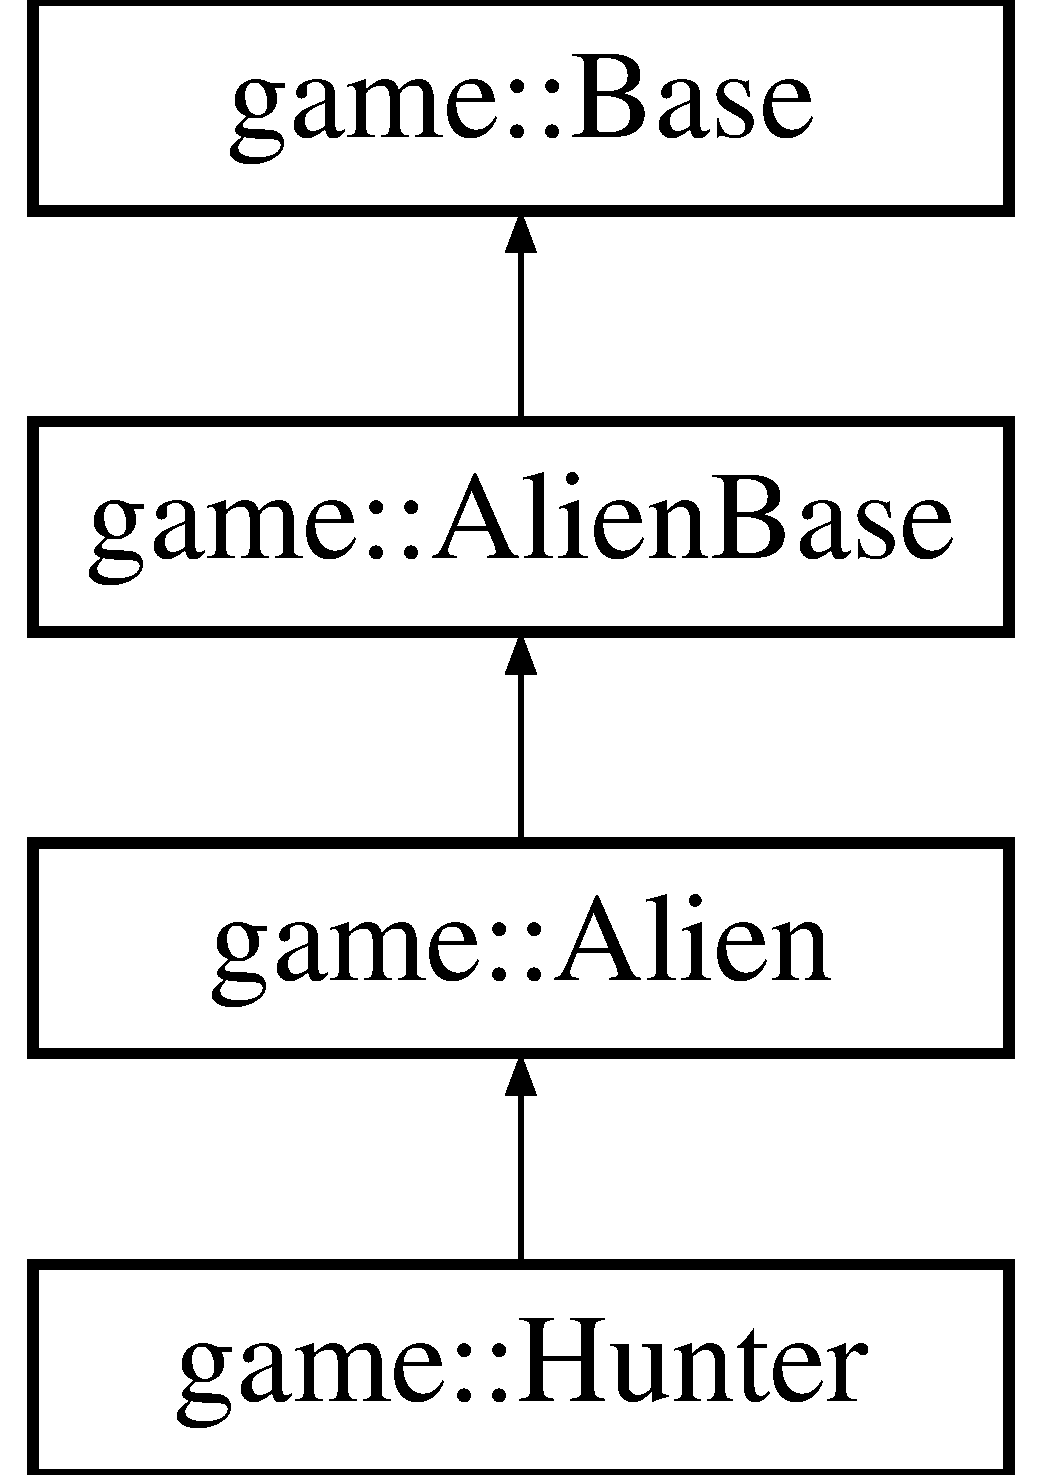
\includegraphics[height=4.000000cm]{classgame_1_1Alien}
\end{center}
\end{figure}
\subsection*{Public Member Functions}
\begin{DoxyCompactItemize}
\item 
\mbox{\Hypertarget{classgame_1_1Alien_ae5772cdffcca2587c44d47adc6d74724}\label{classgame_1_1Alien_ae5772cdffcca2587c44d47adc6d74724}} 
{\bfseries Alien} (Q\+Pixmap image, int x, int y, int velocity, int score, Q\+String base\+Type)
\item 
\mbox{\Hypertarget{classgame_1_1Alien_ac37a3b5d6505bbc63ac74cdf6584cff8}\label{classgame_1_1Alien_ac37a3b5d6505bbc63ac74cdf6584cff8}} 
virtual void {\bfseries move} (Q\+String direction)
\item 
\mbox{\Hypertarget{classgame_1_1Alien_af67d4dec3819a91db7548be3861981c7}\label{classgame_1_1Alien_af67d4dec3819a91db7548be3861981c7}} 
Q\+List$<$ \hyperlink{classgame_1_1Bullet}{Bullet} $\ast$ $>$ {\bfseries shoot} (Q\+String type)
\item 
\mbox{\Hypertarget{classgame_1_1Alien_a9d540a0c44c487f15973149bdbc6097f}\label{classgame_1_1Alien_a9d540a0c44c487f15973149bdbc6097f}} 
virtual Q\+List$<$ \hyperlink{classgame_1_1Bullet}{Bullet} $\ast$ $>$ {\bfseries react} ()
\item 
\mbox{\Hypertarget{classgame_1_1Alien_af52085eda6608a464e997ff4f7b441da}\label{classgame_1_1Alien_af52085eda6608a464e997ff4f7b441da}} 
int {\bfseries get\+\_\+score} () const
\item 
\mbox{\Hypertarget{classgame_1_1Alien_a61256979be794e89e2699bcd54699116}\label{classgame_1_1Alien_a61256979be794e89e2699bcd54699116}} 
Q\+List$<$ \hyperlink{classgame_1_1AlienBase}{Alien\+Base} $\ast$ $>$ {\bfseries get\+Aliens} () const
\item 
\mbox{\Hypertarget{classgame_1_1Alien_a9703a5949b6152a0d8eca6c5fbc2d2dd}\label{classgame_1_1Alien_a9703a5949b6152a0d8eca6c5fbc2d2dd}} 
bool {\bfseries add} (\hyperlink{classgame_1_1AlienBase}{Alien\+Base} $\ast$to\+Add)
\item 
\mbox{\Hypertarget{classgame_1_1Alien_a796c1bf799a1b48b28f8ac78a1926383}\label{classgame_1_1Alien_a796c1bf799a1b48b28f8ac78a1926383}} 
void {\bfseries remove} (\hyperlink{classgame_1_1AlienBase}{Alien\+Base} $\ast$to\+Delete)
\item 
\mbox{\Hypertarget{classgame_1_1Alien_a8bf077a07e4849840f58f861a006f948}\label{classgame_1_1Alien_a8bf077a07e4849840f58f861a006f948}} 
virtual void {\bfseries paint} (Q\+Painter \&painter)
\item 
\mbox{\Hypertarget{classgame_1_1Alien_aa928f035f45b762ab4eeb819a7413450}\label{classgame_1_1Alien_aa928f035f45b762ab4eeb819a7413450}} 
void {\bfseries set\+\_\+y} (int y)
\end{DoxyCompactItemize}
\subsection*{Protected Attributes}
\begin{DoxyCompactItemize}
\item 
\mbox{\Hypertarget{classgame_1_1Alien_a27481624e87c97c483ef69ddbb425d59}\label{classgame_1_1Alien_a27481624e87c97c483ef69ddbb425d59}} 
int {\bfseries velocity}
\item 
\mbox{\Hypertarget{classgame_1_1Alien_a092e336e9db2ad02fd1fa29c6f6812a4}\label{classgame_1_1Alien_a092e336e9db2ad02fd1fa29c6f6812a4}} 
int {\bfseries score}
\item 
\mbox{\Hypertarget{classgame_1_1Alien_a3411d1a2a4c2c7c5141e2ab02a5bff2d}\label{classgame_1_1Alien_a3411d1a2a4c2c7c5141e2ab02a5bff2d}} 
Q\+Sound\+Effect {\bfseries bullet\+S\+FX}
\item 
\mbox{\Hypertarget{classgame_1_1Alien_a60c64a2c8b598ba3f4981f883cd1a02a}\label{classgame_1_1Alien_a60c64a2c8b598ba3f4981f883cd1a02a}} 
\hyperlink{classgame_1_1BulletBuilder}{Bullet\+Builder} {\bfseries builder}
\end{DoxyCompactItemize}


The documentation for this class was generated from the following files\+:\begin{DoxyCompactItemize}
\item 
alien.\+h\item 
alien.\+cpp\end{DoxyCompactItemize}

\hypertarget{classgame_1_1AlienBase}{}\section{game\+:\+:Alien\+Base Class Reference}
\label{classgame_1_1AlienBase}\index{game\+::\+Alien\+Base@{game\+::\+Alien\+Base}}
Inheritance diagram for game\+:\+:Alien\+Base\+:\begin{figure}[H]
\begin{center}
\leavevmode
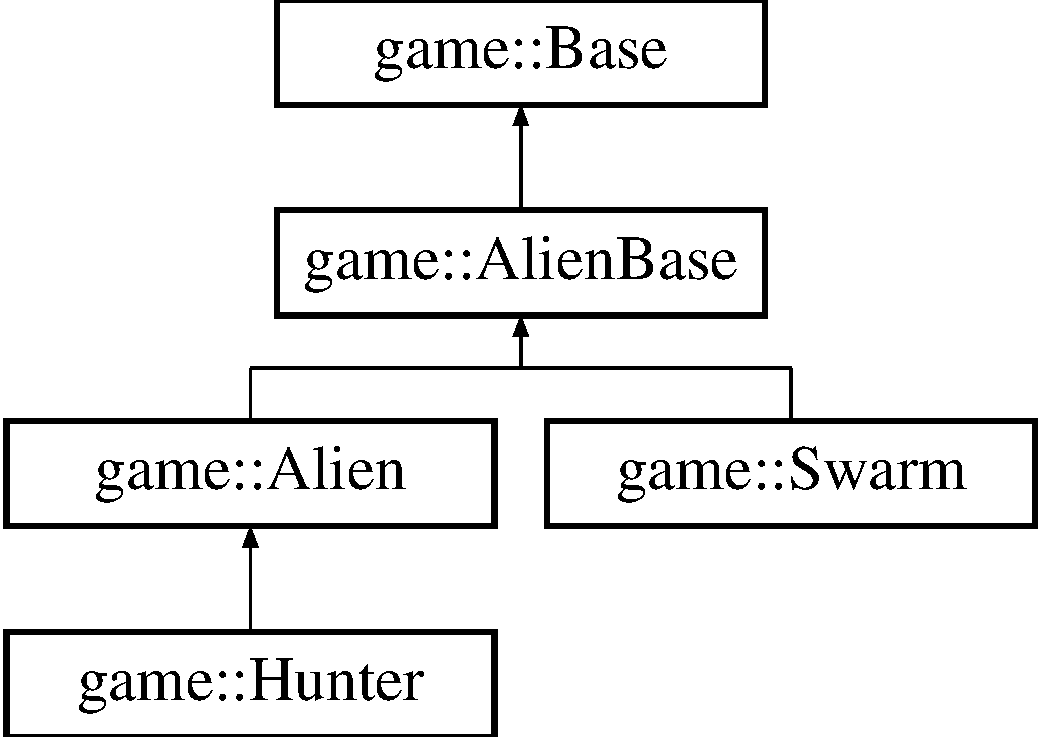
\includegraphics[height=4.000000cm]{classgame_1_1AlienBase}
\end{center}
\end{figure}
\subsection*{Public Member Functions}
\begin{DoxyCompactItemize}
\item 
\mbox{\Hypertarget{classgame_1_1AlienBase_a1262846978fc5ef94b021f86b86c5234}\label{classgame_1_1AlienBase_a1262846978fc5ef94b021f86b86c5234}} 
{\bfseries Alien\+Base} (Q\+Pixmap image, double scale, int x, int y, int window\+Width, int window\+Height, int minX)
\item 
\mbox{\Hypertarget{classgame_1_1AlienBase_ada5b0d95ed3c50ff8808c3cba369a5b7}\label{classgame_1_1AlienBase_ada5b0d95ed3c50ff8808c3cba369a5b7}} 
virtual Q\+List$<$ \hyperlink{classgame_1_1Bullet}{Bullet} $\ast$ $>$ {\bfseries shoot} (Q\+String type)=0
\item 
\mbox{\Hypertarget{classgame_1_1AlienBase_a7aa35de643cd234ca37edb3298b1024d}\label{classgame_1_1AlienBase_a7aa35de643cd234ca37edb3298b1024d}} 
virtual void {\bfseries move} (Q\+String direction)=0
\item 
\mbox{\Hypertarget{classgame_1_1AlienBase_a8ff5abe284c98fe915bfb5f1fcc6cd52}\label{classgame_1_1AlienBase_a8ff5abe284c98fe915bfb5f1fcc6cd52}} 
virtual int {\bfseries get\+\_\+score} () const =0
\item 
\mbox{\Hypertarget{classgame_1_1AlienBase_a5bc585ba514905960d2699780790b3b9}\label{classgame_1_1AlienBase_a5bc585ba514905960d2699780790b3b9}} 
virtual Q\+List$<$ \hyperlink{classgame_1_1AlienBase}{Alien\+Base} $\ast$ $>$ {\bfseries get\+Aliens} () const =0
\item 
\mbox{\Hypertarget{classgame_1_1AlienBase_a2adba0274028ece504be8b574bf72047}\label{classgame_1_1AlienBase_a2adba0274028ece504be8b574bf72047}} 
virtual bool {\bfseries add} (\hyperlink{classgame_1_1AlienBase}{Alien\+Base} $\ast$to\+Add)=0
\item 
\mbox{\Hypertarget{classgame_1_1AlienBase_a580cc448b12a80d495ee21df6b7b54b0}\label{classgame_1_1AlienBase_a580cc448b12a80d495ee21df6b7b54b0}} 
virtual void {\bfseries remove} (\hyperlink{classgame_1_1AlienBase}{Alien\+Base} $\ast$to\+Delete)=0
\item 
\mbox{\Hypertarget{classgame_1_1AlienBase_a6e003cec05ee1fdb2e9181ae0f416670}\label{classgame_1_1AlienBase_a6e003cec05ee1fdb2e9181ae0f416670}} 
virtual Q\+List$<$ \hyperlink{classgame_1_1Bullet}{Bullet} $\ast$ $>$ {\bfseries react} ()=0
\item 
\mbox{\Hypertarget{classgame_1_1AlienBase_a39ed231f233fb4e9e27cd0e4096129bd}\label{classgame_1_1AlienBase_a39ed231f233fb4e9e27cd0e4096129bd}} 
virtual void {\bfseries paint} (Q\+Painter \&painter)=0
\end{DoxyCompactItemize}
\subsection*{Additional Inherited Members}


The documentation for this class was generated from the following files\+:\begin{DoxyCompactItemize}
\item 
alienbase.\+h\item 
composite.\+cpp\end{DoxyCompactItemize}

\hypertarget{classgame_1_1AlienBuilder}{}\section{game\+:\+:Alien\+Builder Class Reference}
\label{classgame_1_1AlienBuilder}\index{game\+::\+Alien\+Builder@{game\+::\+Alien\+Builder}}
\subsection*{Public Member Functions}
\begin{DoxyCompactItemize}
\item 
\mbox{\Hypertarget{classgame_1_1AlienBuilder_ad6c526bde63146a07ee233dcc0539c9b}\label{classgame_1_1AlienBuilder_ad6c526bde63146a07ee233dcc0539c9b}} 
{\bfseries Alien\+Builder} (Q\+Pixmap \&image, Q\+String \&type, \hyperlink{classgame_1_1Base}{Base} \&ship)
\item 
\mbox{\Hypertarget{classgame_1_1AlienBuilder_aecdd1c6a3b297000e1a6b6bc60416650}\label{classgame_1_1AlienBuilder_aecdd1c6a3b297000e1a6b6bc60416650}} 
\hyperlink{classgame_1_1Alien}{Alien} $\ast$ {\bfseries build\+Alien} (Q\+String \&type, int x, int y)
\item 
\mbox{\Hypertarget{classgame_1_1AlienBuilder_a6edbcda3787695657edada653dbe3ce3}\label{classgame_1_1AlienBuilder_a6edbcda3787695657edada653dbe3ce3}} 
int {\bfseries velocity\+Calculator} (Q\+String \&type)
\item 
\mbox{\Hypertarget{classgame_1_1AlienBuilder_ac24663df8d7edc42f69a5ee056a91949}\label{classgame_1_1AlienBuilder_ac24663df8d7edc42f69a5ee056a91949}} 
int {\bfseries score\+Calculator} (Q\+String \&type)
\end{DoxyCompactItemize}
\subsection*{Protected Attributes}
\begin{DoxyCompactItemize}
\item 
\mbox{\Hypertarget{classgame_1_1AlienBuilder_af50d94648522f41480afa57db2450fdf}\label{classgame_1_1AlienBuilder_af50d94648522f41480afa57db2450fdf}} 
Q\+Pixmap {\bfseries image}
\item 
\mbox{\Hypertarget{classgame_1_1AlienBuilder_a20e27658f5a953851271eeb92a81068c}\label{classgame_1_1AlienBuilder_a20e27658f5a953851271eeb92a81068c}} 
Q\+String {\bfseries type}
\item 
\mbox{\Hypertarget{classgame_1_1AlienBuilder_aa446e19ea74df3c79d48f708ff440ad6}\label{classgame_1_1AlienBuilder_aa446e19ea74df3c79d48f708ff440ad6}} 
int {\bfseries score}
\item 
\mbox{\Hypertarget{classgame_1_1AlienBuilder_a3c7d1c90792cfd67e6fbf744b6ebc4ad}\label{classgame_1_1AlienBuilder_a3c7d1c90792cfd67e6fbf744b6ebc4ad}} 
int {\bfseries velocity}
\item 
\mbox{\Hypertarget{classgame_1_1AlienBuilder_a915690fede0ff0a450a0a84d9ecc127b}\label{classgame_1_1AlienBuilder_a915690fede0ff0a450a0a84d9ecc127b}} 
int {\bfseries id}
\end{DoxyCompactItemize}


The documentation for this class was generated from the following files\+:\begin{DoxyCompactItemize}
\item 
alienbuilder.\+h\item 
alienbuilder.\+cpp\end{DoxyCompactItemize}

\hypertarget{classBackground}{}\section{Background Class Reference}
\label{classBackground}\index{Background@{Background}}
\subsection*{Public Member Functions}
\begin{DoxyCompactItemize}
\item 
\mbox{\Hypertarget{classBackground_abfcf8bb350d3dc688b39138f55ace8bf}\label{classBackground_abfcf8bb350d3dc688b39138f55ace8bf}} 
{\bfseries Background} (int screen\+Width, int screen\+Height)
\item 
\mbox{\Hypertarget{classBackground_a36c80fd1a1bfb7f4ffbf7514ae976bc6}\label{classBackground_a36c80fd1a1bfb7f4ffbf7514ae976bc6}} 
void {\bfseries draw} (Q\+Painter $\ast$p)
\item 
\mbox{\Hypertarget{classBackground_aa0fc3036aaf578fc26f6e6a8032a2d27}\label{classBackground_aa0fc3036aaf578fc26f6e6a8032a2d27}} 
void {\bfseries next\+Frame} ()
\end{DoxyCompactItemize}


The documentation for this class was generated from the following files\+:\begin{DoxyCompactItemize}
\item 
background.\+h\item 
background.\+cpp\end{DoxyCompactItemize}

\hypertarget{classgame_1_1BarrierBlock}{}\section{game\+:\+:Barrier\+Block Class Reference}
\label{classgame_1_1BarrierBlock}\index{game\+::\+Barrier\+Block@{game\+::\+Barrier\+Block}}
\subsection*{Public Member Functions}
\begin{DoxyCompactItemize}
\item 
\mbox{\Hypertarget{classgame_1_1BarrierBlock_af749e56fdf63f5a7230dd6f2c8e9bd9b}\label{classgame_1_1BarrierBlock_af749e56fdf63f5a7230dd6f2c8e9bd9b}} 
{\bfseries Barrier\+Block} (int x, int y, unsigned width)
\item 
\mbox{\Hypertarget{classgame_1_1BarrierBlock_af249f2c03b00f7b32a29ee98587b2e31}\label{classgame_1_1BarrierBlock_af249f2c03b00f7b32a29ee98587b2e31}} 
void {\bfseries draw} (Q\+Painter $\ast$p)
\end{DoxyCompactItemize}
\subsection*{Public Attributes}
\begin{DoxyCompactItemize}
\item 
\mbox{\Hypertarget{classgame_1_1BarrierBlock_adcd1902f615bcce1c2fb1dbff5e00192}\label{classgame_1_1BarrierBlock_adcd1902f615bcce1c2fb1dbff5e00192}} 
Q\+Pixmap {\bfseries pixmap}
\item 
\mbox{\Hypertarget{classgame_1_1BarrierBlock_ae553ded7734278dfbc5a9691a81778a3}\label{classgame_1_1BarrierBlock_ae553ded7734278dfbc5a9691a81778a3}} 
int {\bfseries x}
\item 
\mbox{\Hypertarget{classgame_1_1BarrierBlock_a341be367efd9d1617eee8c312baa9ff4}\label{classgame_1_1BarrierBlock_a341be367efd9d1617eee8c312baa9ff4}} 
int {\bfseries y}
\item 
\mbox{\Hypertarget{classgame_1_1BarrierBlock_a0fd20d6c716099bae772dddf3a05aac7}\label{classgame_1_1BarrierBlock_a0fd20d6c716099bae772dddf3a05aac7}} 
unsigned {\bfseries width}
\end{DoxyCompactItemize}


The documentation for this class was generated from the following files\+:\begin{DoxyCompactItemize}
\item 
barrierblock.\+h\item 
barrierblock.\+cpp\end{DoxyCompactItemize}

\hypertarget{classgame_1_1Base}{}\section{game\+:\+:Base Class Reference}
\label{classgame_1_1Base}\index{game\+::\+Base@{game\+::\+Base}}
Inheritance diagram for game\+:\+:Base\+:\begin{figure}[H]
\begin{center}
\leavevmode
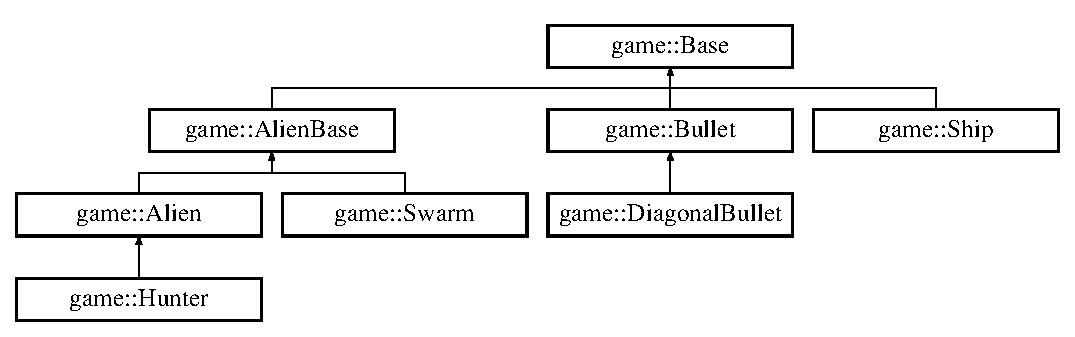
\includegraphics[height=4.000000cm]{classgame_1_1Base}
\end{center}
\end{figure}
\subsection*{Public Member Functions}
\begin{DoxyCompactItemize}
\item 
\mbox{\Hypertarget{classgame_1_1Base_a6fed1f3f4013af8df52b7ae684098eaa}\label{classgame_1_1Base_a6fed1f3f4013af8df52b7ae684098eaa}} 
{\bfseries Base} (Q\+Pixmap image, double scale, int x, int y=0, int boundaryX=800, int boundaryY=600, int minX=0)
\item 
\mbox{\Hypertarget{classgame_1_1Base_acfcb672c526e57890b5b1ef5fca75d09}\label{classgame_1_1Base_acfcb672c526e57890b5b1ef5fca75d09}} 
bool {\bfseries check\+XY} (int x1, int x2, int myX)
\item 
\mbox{\Hypertarget{classgame_1_1Base_a340843de63ea2bc812a9dcfa4e34e9fb}\label{classgame_1_1Base_a340843de63ea2bc812a9dcfa4e34e9fb}} 
bool {\bfseries collides} (int x1, int x2, int y1, int y2)
\item 
\mbox{\Hypertarget{classgame_1_1Base_ae742c89dd481a35971a4f659af0d3745}\label{classgame_1_1Base_ae742c89dd481a35971a4f659af0d3745}} 
bool {\bfseries collides} (\hyperlink{classgame_1_1Base}{Base} \&base)
\item 
\mbox{\Hypertarget{classgame_1_1Base_a4ef01159e220d435dd973c945b802977}\label{classgame_1_1Base_a4ef01159e220d435dd973c945b802977}} 
void {\bfseries set\+\_\+image} (Q\+Pixmap image)
\item 
\mbox{\Hypertarget{classgame_1_1Base_ab96cb70ffa0984d650f8a261663fde92}\label{classgame_1_1Base_ab96cb70ffa0984d650f8a261663fde92}} 
virtual void {\bfseries set\+\_\+x} (int x)
\item 
\mbox{\Hypertarget{classgame_1_1Base_aab1afbed41cd255238a3cc107fe1611e}\label{classgame_1_1Base_aab1afbed41cd255238a3cc107fe1611e}} 
virtual void {\bfseries set\+\_\+y} (int y)
\item 
\mbox{\Hypertarget{classgame_1_1Base_abc4f0e87b3ce03d2b7c0e3cba1505f8c}\label{classgame_1_1Base_abc4f0e87b3ce03d2b7c0e3cba1505f8c}} 
const Q\+Pixmap \& {\bfseries get\+\_\+image} () const
\item 
\mbox{\Hypertarget{classgame_1_1Base_a986b0970cc262be86bfe4337f86f3ba1}\label{classgame_1_1Base_a986b0970cc262be86bfe4337f86f3ba1}} 
double {\bfseries get\+\_\+scale} () const
\item 
\mbox{\Hypertarget{classgame_1_1Base_a9a03e074b91babc5b004467a1749d4b8}\label{classgame_1_1Base_a9a03e074b91babc5b004467a1749d4b8}} 
int {\bfseries get\+\_\+x} () const
\item 
\mbox{\Hypertarget{classgame_1_1Base_ad5016f89e800d05f91fd56c9f16d472e}\label{classgame_1_1Base_ad5016f89e800d05f91fd56c9f16d472e}} 
int {\bfseries get\+\_\+y} () const
\end{DoxyCompactItemize}
\subsection*{Protected Attributes}
\begin{DoxyCompactItemize}
\item 
\mbox{\Hypertarget{classgame_1_1Base_a1e5729a88c5d8693843cd5d8d7f2b041}\label{classgame_1_1Base_a1e5729a88c5d8693843cd5d8d7f2b041}} 
Q\+Pixmap {\bfseries image}
\item 
\mbox{\Hypertarget{classgame_1_1Base_a3a1a3e4d76a32e7c2ecb63e07652319e}\label{classgame_1_1Base_a3a1a3e4d76a32e7c2ecb63e07652319e}} 
int {\bfseries boundaryX}
\item 
\mbox{\Hypertarget{classgame_1_1Base_a6673c7e5dae9e4c5a29e4c2a2bb64b5d}\label{classgame_1_1Base_a6673c7e5dae9e4c5a29e4c2a2bb64b5d}} 
int {\bfseries boundaryY}
\item 
\mbox{\Hypertarget{classgame_1_1Base_a24955d46b4f95d9617859eb7fbf78fe7}\label{classgame_1_1Base_a24955d46b4f95d9617859eb7fbf78fe7}} 
int {\bfseries minX}
\item 
\mbox{\Hypertarget{classgame_1_1Base_a9778a44ad5cdcf606b69d71998284109}\label{classgame_1_1Base_a9778a44ad5cdcf606b69d71998284109}} 
double {\bfseries scale}
\item 
\mbox{\Hypertarget{classgame_1_1Base_aa5c743423c08a054edddae452d84099a}\label{classgame_1_1Base_aa5c743423c08a054edddae452d84099a}} 
int {\bfseries x}
\item 
\mbox{\Hypertarget{classgame_1_1Base_a844bdeed367cd32056e0a289c350a337}\label{classgame_1_1Base_a844bdeed367cd32056e0a289c350a337}} 
int {\bfseries y}
\end{DoxyCompactItemize}


The documentation for this class was generated from the following files\+:\begin{DoxyCompactItemize}
\item 
base.\+h\item 
base.\+cpp\end{DoxyCompactItemize}

\hypertarget{classgame_1_1Bullet}{}\section{game\+:\+:Bullet Class Reference}
\label{classgame_1_1Bullet}\index{game\+::\+Bullet@{game\+::\+Bullet}}
Inheritance diagram for game\+:\+:Bullet\+:\begin{figure}[H]
\begin{center}
\leavevmode
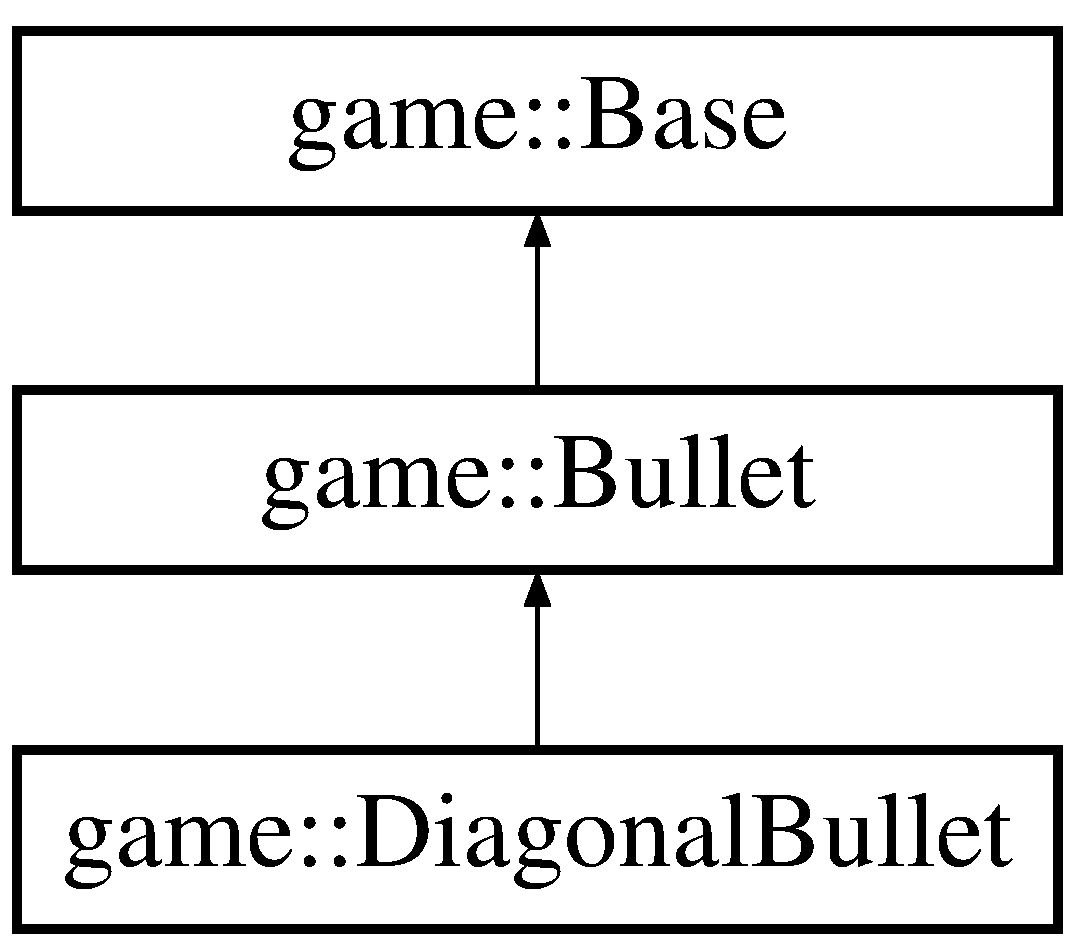
\includegraphics[height=3.000000cm]{classgame_1_1Bullet}
\end{center}
\end{figure}
\subsection*{Public Member Functions}
\begin{DoxyCompactItemize}
\item 
\mbox{\Hypertarget{classgame_1_1Bullet_a275416b258c5e576ad6b6a888808c378}\label{classgame_1_1Bullet_a275416b258c5e576ad6b6a888808c378}} 
{\bfseries Bullet} (Q\+Pixmap image, int x, int y, int bullet\+\_\+velocity, bool friendly)
\item 
\mbox{\Hypertarget{classgame_1_1Bullet_a194930eb9b7a2b49d6011bbd8ea90e93}\label{classgame_1_1Bullet_a194930eb9b7a2b49d6011bbd8ea90e93}} 
virtual void {\bfseries move} ()
\item 
\mbox{\Hypertarget{classgame_1_1Bullet_a8837333b0e26ffa5164ada508227e602}\label{classgame_1_1Bullet_a8837333b0e26ffa5164ada508227e602}} 
int {\bfseries get\+\_\+bullet\+\_\+velocity} () const
\item 
\mbox{\Hypertarget{classgame_1_1Bullet_a64c7d33c678250d10c0a9e30134a3aea}\label{classgame_1_1Bullet_a64c7d33c678250d10c0a9e30134a3aea}} 
bool {\bfseries is\+Friendly} ()
\end{DoxyCompactItemize}
\subsection*{Additional Inherited Members}


The documentation for this class was generated from the following files\+:\begin{DoxyCompactItemize}
\item 
bullet.\+h\item 
bullet.\+cpp\end{DoxyCompactItemize}

\hypertarget{classgame_1_1BulletBuilder}{}\section{game\+:\+:Bullet\+Builder Class Reference}
\label{classgame_1_1BulletBuilder}\index{game\+::\+Bullet\+Builder@{game\+::\+Bullet\+Builder}}
Inheritance diagram for game\+:\+:Bullet\+Builder\+:\begin{figure}[H]
\begin{center}
\leavevmode
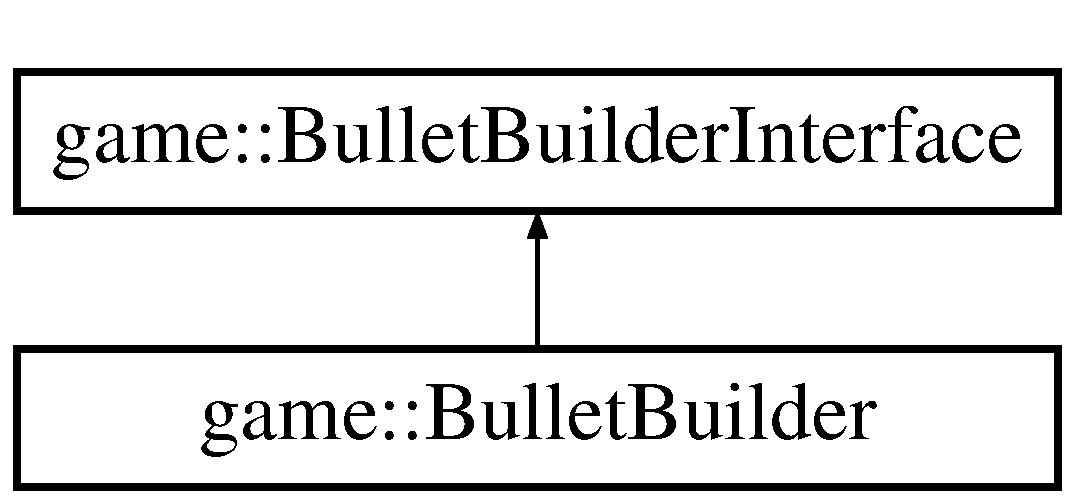
\includegraphics[height=2.000000cm]{classgame_1_1BulletBuilder}
\end{center}
\end{figure}
\subsection*{Public Member Functions}
\begin{DoxyCompactItemize}
\item 
\mbox{\Hypertarget{classgame_1_1BulletBuilder_ac4cacbec8a7ef228330e43a055ae34ea}\label{classgame_1_1BulletBuilder_ac4cacbec8a7ef228330e43a055ae34ea}} 
{\bfseries Bullet\+Builder} (int velocity, \hyperlink{classgame_1_1Base}{Base} \&ship, Q\+String base\+Type, bool friendly)
\item 
\mbox{\Hypertarget{classgame_1_1BulletBuilder_ad09b920f426696cd20f7fa8e663dcbe5}\label{classgame_1_1BulletBuilder_ad09b920f426696cd20f7fa8e663dcbe5}} 
void {\bfseries set\+\_\+velocity} (int velocity)
\item 
\mbox{\Hypertarget{classgame_1_1BulletBuilder_a722a4f9f2fc0ca1658cf04b227af1ee3}\label{classgame_1_1BulletBuilder_a722a4f9f2fc0ca1658cf04b227af1ee3}} 
\hyperlink{classgame_1_1Bullet}{Bullet} $\ast$ {\bfseries build\+\_\+bullet} (Q\+String type)
\end{DoxyCompactItemize}
\subsection*{Protected Member Functions}
\begin{DoxyCompactItemize}
\item 
\mbox{\Hypertarget{classgame_1_1BulletBuilder_a0247bd0b50739729155d74f28b34e883}\label{classgame_1_1BulletBuilder_a0247bd0b50739729155d74f28b34e883}} 
Q\+Pixmap {\bfseries calculate\+\_\+image} (Q\+String \&type)
\end{DoxyCompactItemize}
\subsection*{Protected Attributes}
\begin{DoxyCompactItemize}
\item 
\mbox{\Hypertarget{classgame_1_1BulletBuilder_ad04dd50b078c62404ee4dc4985215b2e}\label{classgame_1_1BulletBuilder_ad04dd50b078c62404ee4dc4985215b2e}} 
bool {\bfseries friendly}
\item 
\mbox{\Hypertarget{classgame_1_1BulletBuilder_a19da7e0a10986ed821bb8456ae5d93de}\label{classgame_1_1BulletBuilder_a19da7e0a10986ed821bb8456ae5d93de}} 
int {\bfseries velocity}
\item 
\mbox{\Hypertarget{classgame_1_1BulletBuilder_a3fdce5bd8b1c34048dbff0ff962a6c0a}\label{classgame_1_1BulletBuilder_a3fdce5bd8b1c34048dbff0ff962a6c0a}} 
Q\+Pixmap {\bfseries image}
\item 
\mbox{\Hypertarget{classgame_1_1BulletBuilder_a2af27dd173fadd5aef7d49752d649e16}\label{classgame_1_1BulletBuilder_a2af27dd173fadd5aef7d49752d649e16}} 
Q\+String {\bfseries base\+Type}
\item 
\mbox{\Hypertarget{classgame_1_1BulletBuilder_afb44969f55ed129aadeddfc9b5ea5f63}\label{classgame_1_1BulletBuilder_afb44969f55ed129aadeddfc9b5ea5f63}} 
\hyperlink{classgame_1_1Base}{Base} \& {\bfseries ship}
\end{DoxyCompactItemize}


The documentation for this class was generated from the following files\+:\begin{DoxyCompactItemize}
\item 
bulletbuilder.\+h\item 
bulletbuilder.\+cpp\end{DoxyCompactItemize}

\hypertarget{classgame_1_1BulletBuilderInterface}{}\section{game\+:\+:Bullet\+Builder\+Interface Class Reference}
\label{classgame_1_1BulletBuilderInterface}\index{game\+::\+Bullet\+Builder\+Interface@{game\+::\+Bullet\+Builder\+Interface}}
Inheritance diagram for game\+:\+:Bullet\+Builder\+Interface\+:\begin{figure}[H]
\begin{center}
\leavevmode
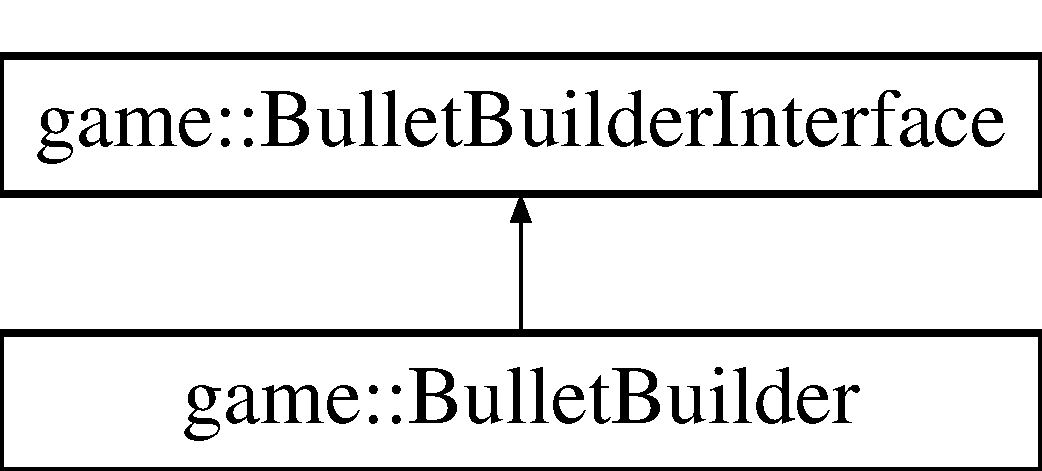
\includegraphics[height=2.000000cm]{classgame_1_1BulletBuilderInterface}
\end{center}
\end{figure}
\subsection*{Public Member Functions}
\begin{DoxyCompactItemize}
\item 
\mbox{\Hypertarget{classgame_1_1BulletBuilderInterface_a25012860935bc4de6c55cad9490275e9}\label{classgame_1_1BulletBuilderInterface_a25012860935bc4de6c55cad9490275e9}} 
virtual \hyperlink{classgame_1_1Bullet}{Bullet} $\ast$ {\bfseries build\+\_\+bullet} (Q\+String type)=0
\item 
\mbox{\Hypertarget{classgame_1_1BulletBuilderInterface_a983cefa4614cd88c453c8761793b43d8}\label{classgame_1_1BulletBuilderInterface_a983cefa4614cd88c453c8761793b43d8}} 
virtual void {\bfseries set\+\_\+velocity} (int velocity)=0
\end{DoxyCompactItemize}


The documentation for this class was generated from the following file\+:\begin{DoxyCompactItemize}
\item 
bulletbuilderinterface.\+h\end{DoxyCompactItemize}

\hypertarget{classgame_1_1Command}{}\section{game\+:\+:Command Class Reference}
\label{classgame_1_1Command}\index{game\+::\+Command@{game\+::\+Command}}
Inheritance diagram for game\+:\+:Command\+:\begin{figure}[H]
\begin{center}
\leavevmode
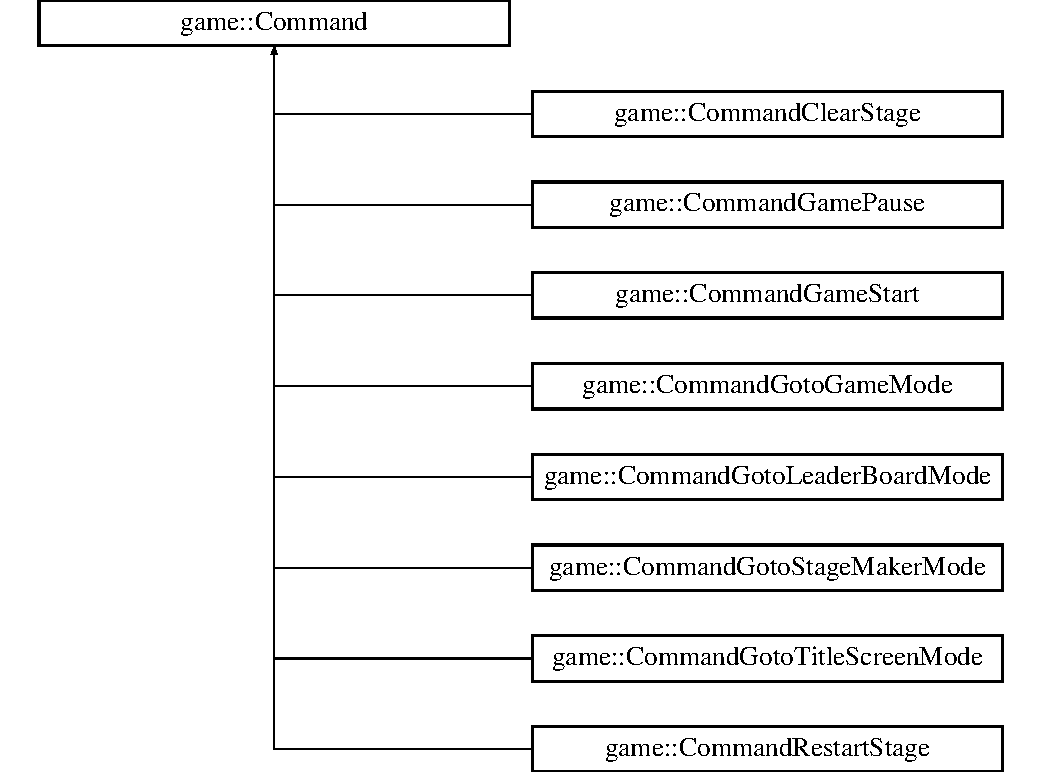
\includegraphics[height=9.000000cm]{classgame_1_1Command}
\end{center}
\end{figure}
\subsection*{Public Member Functions}
\begin{DoxyCompactItemize}
\item 
\mbox{\Hypertarget{classgame_1_1Command_aa2e0454851b0226dcd470f358c79206b}\label{classgame_1_1Command_aa2e0454851b0226dcd470f358c79206b}} 
{\bfseries Command} (\hyperlink{classgame_1_1GameDialog}{Game\+Dialog} $\ast$gamedialog)
\item 
\mbox{\Hypertarget{classgame_1_1Command_a783331d21aa8d909c40ad4f75a228aad}\label{classgame_1_1Command_a783331d21aa8d909c40ad4f75a228aad}} 
virtual void {\bfseries execute} ()=0
\end{DoxyCompactItemize}
\subsection*{Protected Attributes}
\begin{DoxyCompactItemize}
\item 
\mbox{\Hypertarget{classgame_1_1Command_a0b597e617248e801486c7a614e5e7d1e}\label{classgame_1_1Command_a0b597e617248e801486c7a614e5e7d1e}} 
\hyperlink{classgame_1_1GameDialog}{Game\+Dialog} $\ast$ {\bfseries g\+Dialog}
\end{DoxyCompactItemize}


The documentation for this class was generated from the following file\+:\begin{DoxyCompactItemize}
\item 
command.\+h\end{DoxyCompactItemize}

\hypertarget{classgame_1_1CommandClearStage}{}\section{game\+:\+:Command\+Clear\+Stage Class Reference}
\label{classgame_1_1CommandClearStage}\index{game\+::\+Command\+Clear\+Stage@{game\+::\+Command\+Clear\+Stage}}
Inheritance diagram for game\+:\+:Command\+Clear\+Stage\+:\begin{figure}[H]
\begin{center}
\leavevmode
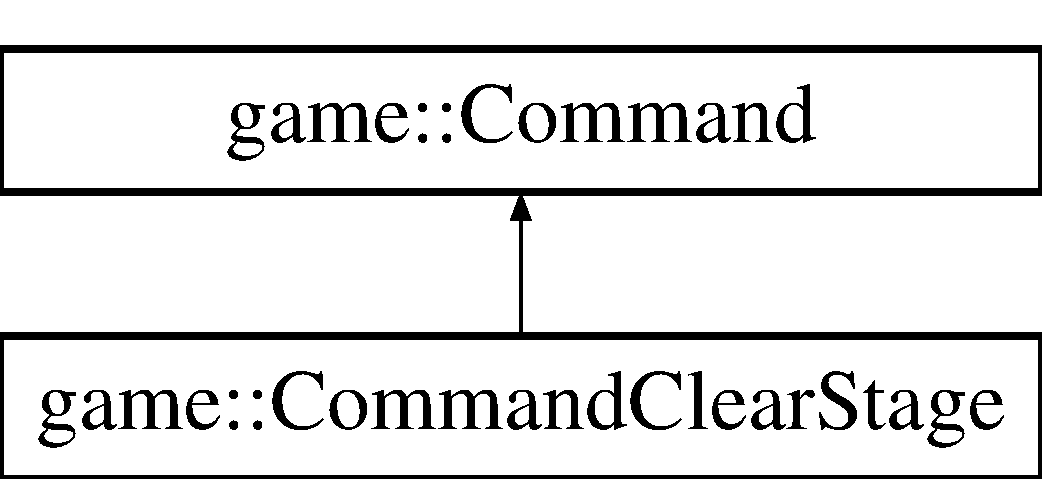
\includegraphics[height=2.000000cm]{classgame_1_1CommandClearStage}
\end{center}
\end{figure}
\subsection*{Public Member Functions}
\begin{DoxyCompactItemize}
\item 
\mbox{\Hypertarget{classgame_1_1CommandClearStage_a1e7dafd0c15118746360bfd95d22815f}\label{classgame_1_1CommandClearStage_a1e7dafd0c15118746360bfd95d22815f}} 
{\bfseries Command\+Clear\+Stage} (\hyperlink{classgame_1_1GameDialog}{Game\+Dialog} $\ast$gamedialog)
\item 
\mbox{\Hypertarget{classgame_1_1CommandClearStage_ab53d909ad9c842f3c04710fb59abc308}\label{classgame_1_1CommandClearStage_ab53d909ad9c842f3c04710fb59abc308}} 
virtual void {\bfseries execute} ()
\end{DoxyCompactItemize}
\subsection*{Additional Inherited Members}


The documentation for this class was generated from the following files\+:\begin{DoxyCompactItemize}
\item 
commandclearstage.\+h\item 
commandclearstage.\+cpp\end{DoxyCompactItemize}

\hypertarget{classgame_1_1CommandGamePause}{}\section{game\+:\+:Command\+Game\+Pause Class Reference}
\label{classgame_1_1CommandGamePause}\index{game\+::\+Command\+Game\+Pause@{game\+::\+Command\+Game\+Pause}}
Inheritance diagram for game\+:\+:Command\+Game\+Pause\+:\begin{figure}[H]
\begin{center}
\leavevmode
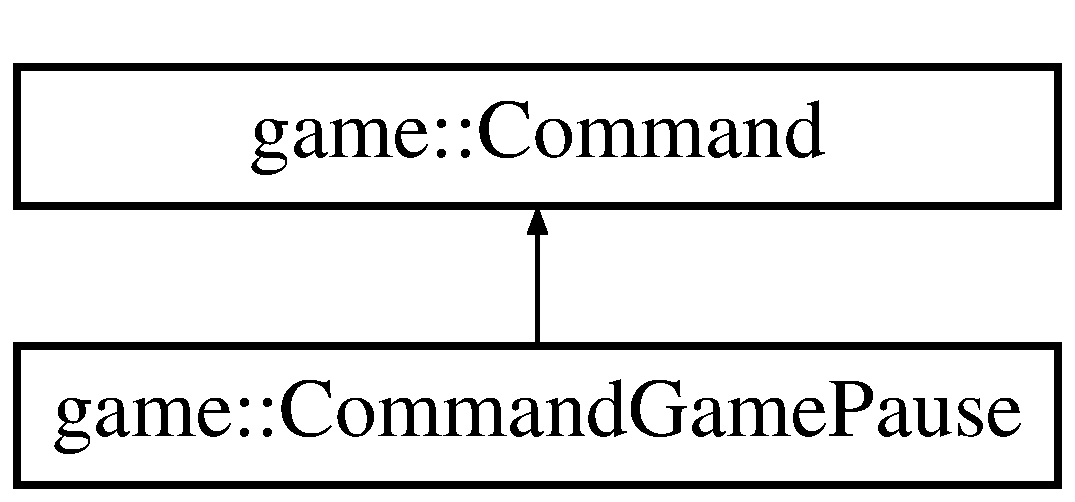
\includegraphics[height=2.000000cm]{classgame_1_1CommandGamePause}
\end{center}
\end{figure}
\subsection*{Public Member Functions}
\begin{DoxyCompactItemize}
\item 
\mbox{\Hypertarget{classgame_1_1CommandGamePause_a033daa0923ecfc63619961a72b67e2cc}\label{classgame_1_1CommandGamePause_a033daa0923ecfc63619961a72b67e2cc}} 
{\bfseries Command\+Game\+Pause} (\hyperlink{classgame_1_1GameDialog}{Game\+Dialog} $\ast$gamedialog)
\item 
\mbox{\Hypertarget{classgame_1_1CommandGamePause_ae5a44637c33c29589300cf2e898506d5}\label{classgame_1_1CommandGamePause_ae5a44637c33c29589300cf2e898506d5}} 
virtual void {\bfseries execute} ()
\end{DoxyCompactItemize}
\subsection*{Additional Inherited Members}


The documentation for this class was generated from the following files\+:\begin{DoxyCompactItemize}
\item 
commandgamepause.\+h\item 
commandgamepause.\+cpp\end{DoxyCompactItemize}

\hypertarget{classgame_1_1CommandGameStart}{}\section{game\+:\+:Command\+Game\+Start Class Reference}
\label{classgame_1_1CommandGameStart}\index{game\+::\+Command\+Game\+Start@{game\+::\+Command\+Game\+Start}}
Inheritance diagram for game\+:\+:Command\+Game\+Start\+:\begin{figure}[H]
\begin{center}
\leavevmode
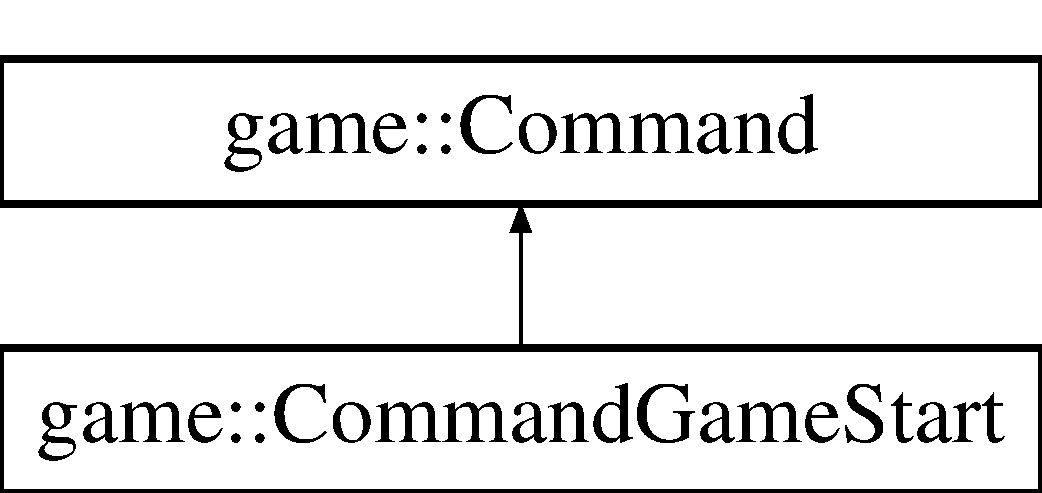
\includegraphics[height=2.000000cm]{classgame_1_1CommandGameStart}
\end{center}
\end{figure}
\subsection*{Public Member Functions}
\begin{DoxyCompactItemize}
\item 
\mbox{\Hypertarget{classgame_1_1CommandGameStart_a206580f2f617c056dd8ed1b3e1717eb4}\label{classgame_1_1CommandGameStart_a206580f2f617c056dd8ed1b3e1717eb4}} 
{\bfseries Command\+Game\+Start} (\hyperlink{classgame_1_1GameDialog}{Game\+Dialog} $\ast$gamedialog)
\item 
\mbox{\Hypertarget{classgame_1_1CommandGameStart_a129ae7102d5d2ebb84e70ecb5a6ee55c}\label{classgame_1_1CommandGameStart_a129ae7102d5d2ebb84e70ecb5a6ee55c}} 
virtual void {\bfseries execute} ()
\end{DoxyCompactItemize}
\subsection*{Additional Inherited Members}


The documentation for this class was generated from the following files\+:\begin{DoxyCompactItemize}
\item 
commandgamestart.\+h\item 
commandgamestart.\+cpp\end{DoxyCompactItemize}

\hypertarget{classgame_1_1CommandGotoGameMode}{}\section{game\+:\+:Command\+Goto\+Game\+Mode Class Reference}
\label{classgame_1_1CommandGotoGameMode}\index{game\+::\+Command\+Goto\+Game\+Mode@{game\+::\+Command\+Goto\+Game\+Mode}}
Inheritance diagram for game\+:\+:Command\+Goto\+Game\+Mode\+:\begin{figure}[H]
\begin{center}
\leavevmode
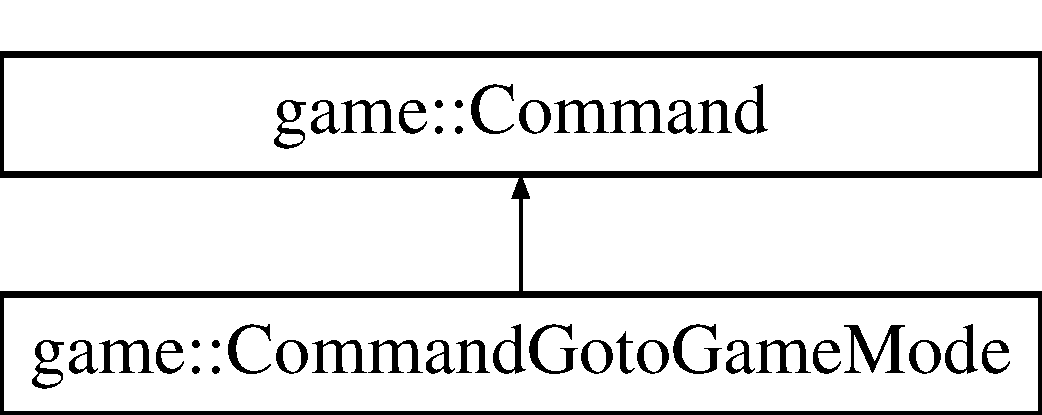
\includegraphics[height=2.000000cm]{classgame_1_1CommandGotoGameMode}
\end{center}
\end{figure}
\subsection*{Public Member Functions}
\begin{DoxyCompactItemize}
\item 
\mbox{\Hypertarget{classgame_1_1CommandGotoGameMode_a561a417ea502150f313caefe7a2fcfdd}\label{classgame_1_1CommandGotoGameMode_a561a417ea502150f313caefe7a2fcfdd}} 
{\bfseries Command\+Goto\+Game\+Mode} (\hyperlink{classgame_1_1GameDialog}{Game\+Dialog} $\ast$gamedialog)
\item 
\mbox{\Hypertarget{classgame_1_1CommandGotoGameMode_a19a17714630bc986ebaa713ffd64224f}\label{classgame_1_1CommandGotoGameMode_a19a17714630bc986ebaa713ffd64224f}} 
virtual void {\bfseries execute} ()
\end{DoxyCompactItemize}
\subsection*{Additional Inherited Members}


The documentation for this class was generated from the following files\+:\begin{DoxyCompactItemize}
\item 
commandgotogamemode.\+h\item 
commandgotogamemode.\+cpp\end{DoxyCompactItemize}

\hypertarget{classgame_1_1CommandGotoLeaderBoardMode}{}\section{game\+:\+:Command\+Goto\+Leader\+Board\+Mode Class Reference}
\label{classgame_1_1CommandGotoLeaderBoardMode}\index{game\+::\+Command\+Goto\+Leader\+Board\+Mode@{game\+::\+Command\+Goto\+Leader\+Board\+Mode}}
Inheritance diagram for game\+:\+:Command\+Goto\+Leader\+Board\+Mode\+:\begin{figure}[H]
\begin{center}
\leavevmode
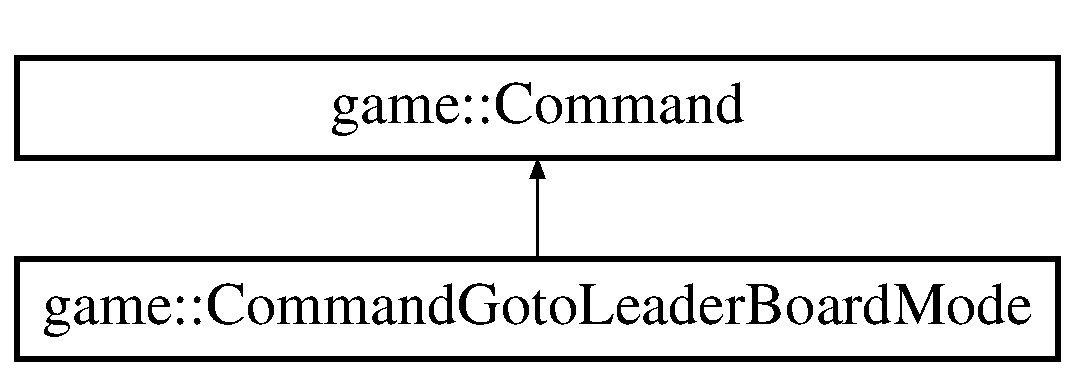
\includegraphics[height=2.000000cm]{classgame_1_1CommandGotoLeaderBoardMode}
\end{center}
\end{figure}
\subsection*{Public Member Functions}
\begin{DoxyCompactItemize}
\item 
\mbox{\Hypertarget{classgame_1_1CommandGotoLeaderBoardMode_aec26d3b15f46a80fb10014dde9f704be}\label{classgame_1_1CommandGotoLeaderBoardMode_aec26d3b15f46a80fb10014dde9f704be}} 
{\bfseries Command\+Goto\+Leader\+Board\+Mode} (\hyperlink{classgame_1_1GameDialog}{Game\+Dialog} $\ast$gamedialog)
\item 
\mbox{\Hypertarget{classgame_1_1CommandGotoLeaderBoardMode_a9ec6c7778ff5e2b687f8e5558c330afe}\label{classgame_1_1CommandGotoLeaderBoardMode_a9ec6c7778ff5e2b687f8e5558c330afe}} 
virtual void {\bfseries execute} ()
\end{DoxyCompactItemize}
\subsection*{Additional Inherited Members}


The documentation for this class was generated from the following files\+:\begin{DoxyCompactItemize}
\item 
commandgotoleaderboardmode.\+h\item 
commandgotoleaderboardmode.\+cpp\end{DoxyCompactItemize}

\hypertarget{classgame_1_1CommandGotoStageMakerMode}{}\section{game\+:\+:Command\+Goto\+Stage\+Maker\+Mode Class Reference}
\label{classgame_1_1CommandGotoStageMakerMode}\index{game\+::\+Command\+Goto\+Stage\+Maker\+Mode@{game\+::\+Command\+Goto\+Stage\+Maker\+Mode}}
Inheritance diagram for game\+:\+:Command\+Goto\+Stage\+Maker\+Mode\+:\begin{figure}[H]
\begin{center}
\leavevmode
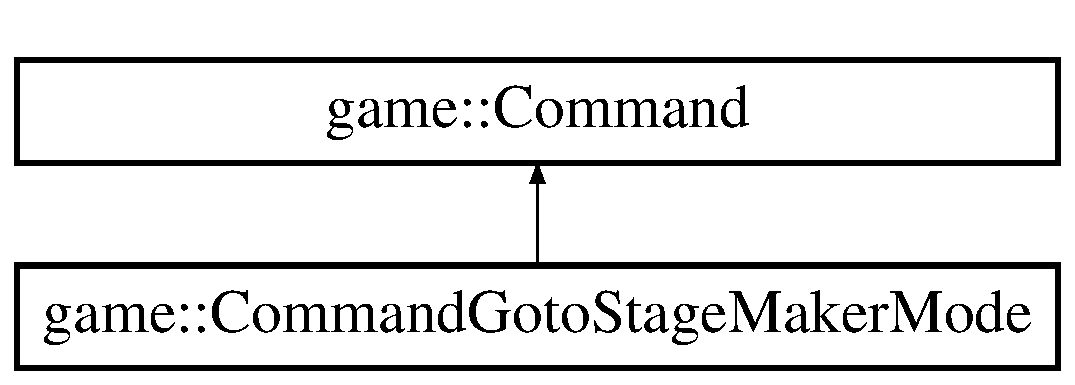
\includegraphics[height=2.000000cm]{classgame_1_1CommandGotoStageMakerMode}
\end{center}
\end{figure}
\subsection*{Public Member Functions}
\begin{DoxyCompactItemize}
\item 
\mbox{\Hypertarget{classgame_1_1CommandGotoStageMakerMode_ac25c4399221f8eea3ab61f1172190137}\label{classgame_1_1CommandGotoStageMakerMode_ac25c4399221f8eea3ab61f1172190137}} 
{\bfseries Command\+Goto\+Stage\+Maker\+Mode} (\hyperlink{classgame_1_1GameDialog}{Game\+Dialog} $\ast$gamedialog)
\item 
\mbox{\Hypertarget{classgame_1_1CommandGotoStageMakerMode_a1f4a37f00c73f76cfb50650e0aefcbf8}\label{classgame_1_1CommandGotoStageMakerMode_a1f4a37f00c73f76cfb50650e0aefcbf8}} 
virtual void {\bfseries execute} ()
\end{DoxyCompactItemize}
\subsection*{Additional Inherited Members}


The documentation for this class was generated from the following files\+:\begin{DoxyCompactItemize}
\item 
commandgotostagemakermode.\+h\item 
commandgotostagemakermode.\+cpp\end{DoxyCompactItemize}

\hypertarget{classgame_1_1CommandGotoTitleScreenMode}{}\section{game\+:\+:Command\+Goto\+Title\+Screen\+Mode Class Reference}
\label{classgame_1_1CommandGotoTitleScreenMode}\index{game\+::\+Command\+Goto\+Title\+Screen\+Mode@{game\+::\+Command\+Goto\+Title\+Screen\+Mode}}
Inheritance diagram for game\+:\+:Command\+Goto\+Title\+Screen\+Mode\+:\begin{figure}[H]
\begin{center}
\leavevmode
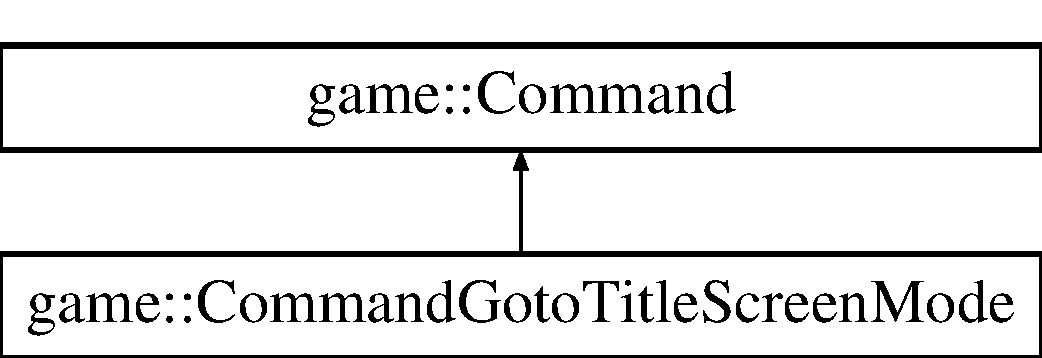
\includegraphics[height=2.000000cm]{classgame_1_1CommandGotoTitleScreenMode}
\end{center}
\end{figure}
\subsection*{Public Member Functions}
\begin{DoxyCompactItemize}
\item 
\mbox{\Hypertarget{classgame_1_1CommandGotoTitleScreenMode_a4eb22eb11ea1b38493a56cf632c0f48e}\label{classgame_1_1CommandGotoTitleScreenMode_a4eb22eb11ea1b38493a56cf632c0f48e}} 
{\bfseries Command\+Goto\+Title\+Screen\+Mode} (\hyperlink{classgame_1_1GameDialog}{Game\+Dialog} $\ast$gamedialog)
\item 
\mbox{\Hypertarget{classgame_1_1CommandGotoTitleScreenMode_afa16f2f39d1009c82b5a5a8012380f15}\label{classgame_1_1CommandGotoTitleScreenMode_afa16f2f39d1009c82b5a5a8012380f15}} 
virtual void {\bfseries execute} ()
\end{DoxyCompactItemize}
\subsection*{Additional Inherited Members}


The documentation for this class was generated from the following files\+:\begin{DoxyCompactItemize}
\item 
commandgototitlescreenmode.\+h\item 
commandgototitlescreenmode.\+cpp\end{DoxyCompactItemize}

\hypertarget{classgame_1_1CommandRestartStage}{}\section{game\+:\+:Command\+Restart\+Stage Class Reference}
\label{classgame_1_1CommandRestartStage}\index{game\+::\+Command\+Restart\+Stage@{game\+::\+Command\+Restart\+Stage}}
Inheritance diagram for game\+:\+:Command\+Restart\+Stage\+:\begin{figure}[H]
\begin{center}
\leavevmode
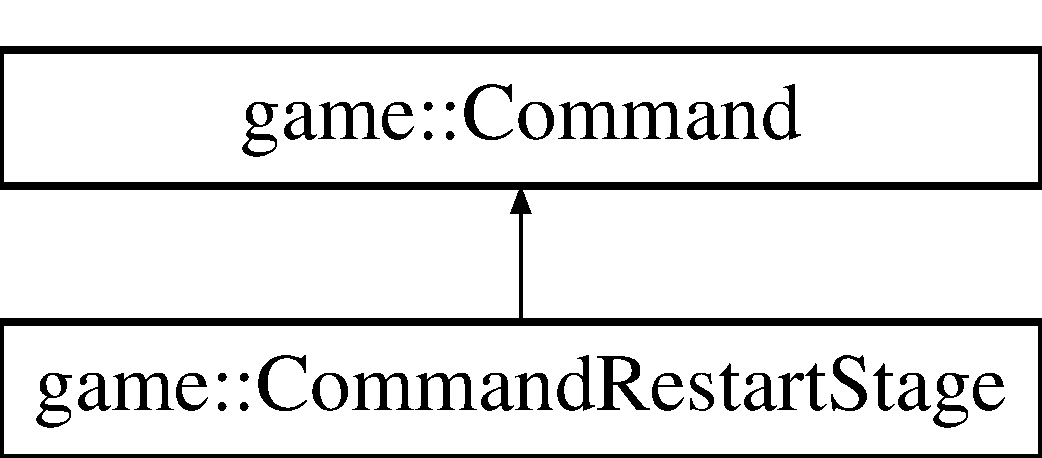
\includegraphics[height=2.000000cm]{classgame_1_1CommandRestartStage}
\end{center}
\end{figure}
\subsection*{Public Member Functions}
\begin{DoxyCompactItemize}
\item 
\mbox{\Hypertarget{classgame_1_1CommandRestartStage_acd8a536da4a5bca3fad8f6c948ce7a94}\label{classgame_1_1CommandRestartStage_acd8a536da4a5bca3fad8f6c948ce7a94}} 
{\bfseries Command\+Restart\+Stage} (\hyperlink{classgame_1_1GameDialog}{Game\+Dialog} $\ast$gamedialog)
\item 
\mbox{\Hypertarget{classgame_1_1CommandRestartStage_ab4d9da97ff5958220cae2c952695ee1f}\label{classgame_1_1CommandRestartStage_ab4d9da97ff5958220cae2c952695ee1f}} 
virtual void {\bfseries execute} ()
\end{DoxyCompactItemize}
\subsection*{Additional Inherited Members}


The documentation for this class was generated from the following files\+:\begin{DoxyCompactItemize}
\item 
commonrestartstage.\+h\item 
commonrestartstage.\+cpp\end{DoxyCompactItemize}

\hypertarget{classgame_1_1Config}{}\section{game\+:\+:Config Class Reference}
\label{classgame_1_1Config}\index{game\+::\+Config@{game\+::\+Config}}
\subsection*{Public Member Functions}
\begin{DoxyCompactItemize}
\item 
\mbox{\Hypertarget{classgame_1_1Config_aaa28fbdf3d41f3f328178c6d5f600dd9}\label{classgame_1_1Config_aaa28fbdf3d41f3f328178c6d5f600dd9}} 
Q\+String {\bfseries get\+\_\+name} ()
\item 
\mbox{\Hypertarget{classgame_1_1Config_af4786d89e182b04fdc5381d0f026246f}\label{classgame_1_1Config_af4786d89e182b04fdc5381d0f026246f}} 
double {\bfseries get\+\_\+scale} ()
\item 
\mbox{\Hypertarget{classgame_1_1Config_a31429fda8ce34409b92fc05cc418f3d9}\label{classgame_1_1Config_a31429fda8ce34409b92fc05cc418f3d9}} 
int {\bfseries get\+\_\+startpos} ()
\item 
\mbox{\Hypertarget{classgame_1_1Config_a433e55f6acf9ed182c385be1acf7192a}\label{classgame_1_1Config_a433e55f6acf9ed182c385be1acf7192a}} 
Q\+String\+List {\bfseries get\+\_\+instructs} ()
\item 
\mbox{\Hypertarget{classgame_1_1Config_ae0a829cf9b316fa80aa75b4033cbaf9d}\label{classgame_1_1Config_ae0a829cf9b316fa80aa75b4033cbaf9d}} 
std\+::vector$<$ Q\+List$<$ \hyperlink{classgame_1_1SwarmInfo}{Swarm\+Info} $>$ $>$ {\bfseries get\+Swarm\+List} ()
\item 
\mbox{\Hypertarget{classgame_1_1Config_a800502a13dde9c77704f84edce0bd8cb}\label{classgame_1_1Config_a800502a13dde9c77704f84edce0bd8cb}} 
int {\bfseries get\+\_\+frames} ()
\item 
\mbox{\Hypertarget{classgame_1_1Config_a06ecefbce47873f8522064d849746661}\label{classgame_1_1Config_a06ecefbce47873f8522064d849746661}} 
int {\bfseries get\+\_\+\+S\+C\+A\+L\+E\+D\+W\+I\+D\+TH} ()
\item 
\mbox{\Hypertarget{classgame_1_1Config_aecf22ed360bb9410c932baa9534b8450}\label{classgame_1_1Config_aecf22ed360bb9410c932baa9534b8450}} 
int {\bfseries get\+\_\+\+S\+C\+A\+L\+E\+D\+H\+E\+I\+G\+HT} ()
\end{DoxyCompactItemize}
\subsection*{Static Public Member Functions}
\begin{DoxyCompactItemize}
\item 
\mbox{\Hypertarget{classgame_1_1Config_a0920ff53c42bdb9b38499d5f06f77cea}\label{classgame_1_1Config_a0920ff53c42bdb9b38499d5f06f77cea}} 
static \hyperlink{classgame_1_1Config}{Config} $\ast$ {\bfseries get\+Instance} ()
\end{DoxyCompactItemize}
\subsection*{Public Attributes}
\begin{DoxyCompactItemize}
\item 
\mbox{\Hypertarget{classgame_1_1Config_ae391a4ba5131c1a5d43b7a8024af43aa}\label{classgame_1_1Config_ae391a4ba5131c1a5d43b7a8024af43aa}} 
bool {\bfseries ship\+Use\+Xwing}
\end{DoxyCompactItemize}


The documentation for this class was generated from the following files\+:\begin{DoxyCompactItemize}
\item 
config.\+h\item 
config.\+cpp\end{DoxyCompactItemize}

\hypertarget{classgame_1_1Cursor}{}\section{game\+:\+:Cursor Class Reference}
\label{classgame_1_1Cursor}\index{game\+::\+Cursor@{game\+::\+Cursor}}
\subsection*{Public Member Functions}
\begin{DoxyCompactItemize}
\item 
\mbox{\Hypertarget{classgame_1_1Cursor_a9ad1627496feb7657d543f3c97f3f257}\label{classgame_1_1Cursor_a9ad1627496feb7657d543f3c97f3f257}} 
{\bfseries Cursor} (\hyperlink{classgame_1_1GameDialog}{Game\+Dialog} $\ast$g\+Dialog)
\item 
\mbox{\Hypertarget{classgame_1_1Cursor_a575adecc55a1a2016665e2ba3ce98926}\label{classgame_1_1Cursor_a575adecc55a1a2016665e2ba3ce98926}} 
\hyperlink{classgame_1_1CursorState}{Cursor\+State} $\ast$ {\bfseries get\+Cur\+State} ()
\item 
\mbox{\Hypertarget{classgame_1_1Cursor_af2bd780f93874d177d93db3fe381665f}\label{classgame_1_1Cursor_af2bd780f93874d177d93db3fe381665f}} 
void {\bfseries set\+Cursor\+State} (C\+U\+R\+S\+O\+R\+\_\+\+S\+T\+A\+TE state)
\end{DoxyCompactItemize}
\subsection*{Public Attributes}
\begin{DoxyCompactItemize}
\item 
\mbox{\Hypertarget{classgame_1_1Cursor_a50c0c4ad740ebd7529c22c4bb7f94206}\label{classgame_1_1Cursor_a50c0c4ad740ebd7529c22c4bb7f94206}} 
int {\bfseries radius}
\item 
\mbox{\Hypertarget{classgame_1_1Cursor_a694099e5d3c5909ddb7b8f54082c74d6}\label{classgame_1_1Cursor_a694099e5d3c5909ddb7b8f54082c74d6}} 
C\+U\+R\+S\+O\+R\+\_\+\+S\+T\+A\+TE {\bfseries state}
\item 
\mbox{\Hypertarget{classgame_1_1Cursor_aa0acb0a05afd3a037ed3af9a8afa7949}\label{classgame_1_1Cursor_aa0acb0a05afd3a037ed3af9a8afa7949}} 
C\+U\+R\+S\+O\+R\+\_\+\+S\+T\+A\+TE {\bfseries pre\+State}
\item 
\mbox{\Hypertarget{classgame_1_1Cursor_a50aaaa67c87c62315901e4f97a5e3049}\label{classgame_1_1Cursor_a50aaaa67c87c62315901e4f97a5e3049}} 
\hyperlink{classgame_1_1CursorState}{Cursor\+State} $\ast$ {\bfseries current\+State}
\item 
\mbox{\Hypertarget{classgame_1_1Cursor_adee1bb58f743e9c346c981f7b697ae0e}\label{classgame_1_1Cursor_adee1bb58f743e9c346c981f7b697ae0e}} 
std\+::map$<$ C\+U\+R\+S\+O\+R\+\_\+\+S\+T\+A\+TE, \hyperlink{classgame_1_1CursorState}{Cursor\+State} $\ast$ $>$ {\bfseries cursor\+States\+List}
\end{DoxyCompactItemize}


The documentation for this class was generated from the following files\+:\begin{DoxyCompactItemize}
\item 
cursor.\+h\item 
cursor.\+cpp\end{DoxyCompactItemize}

\hypertarget{classgame_1_1CursorState}{}\section{game\+:\+:Cursor\+State Class Reference}
\label{classgame_1_1CursorState}\index{game\+::\+Cursor\+State@{game\+::\+Cursor\+State}}
Inheritance diagram for game\+:\+:Cursor\+State\+:\begin{figure}[H]
\begin{center}
\leavevmode
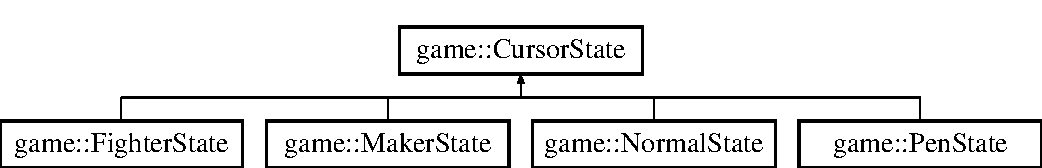
\includegraphics[height=2.000000cm]{classgame_1_1CursorState}
\end{center}
\end{figure}
\subsection*{Public Member Functions}
\begin{DoxyCompactItemize}
\item 
\mbox{\Hypertarget{classgame_1_1CursorState_acd2a923f1ab53c7e89343fcf68afb090}\label{classgame_1_1CursorState_acd2a923f1ab53c7e89343fcf68afb090}} 
{\bfseries Cursor\+State} (\hyperlink{classgame_1_1Cursor}{Cursor} $\ast$c, \hyperlink{classgame_1_1GameDialog}{Game\+Dialog} $\ast$g\+Dialog)
\item 
\mbox{\Hypertarget{classgame_1_1CursorState_aae2cb6cb2261d9a4c5919ac61e03e6ee}\label{classgame_1_1CursorState_aae2cb6cb2261d9a4c5919ac61e03e6ee}} 
virtual void {\bfseries process\+Mouse\+Event} (Q\+Mouse\+Event $\ast$event)=0
\item 
\mbox{\Hypertarget{classgame_1_1CursorState_ac962db2f670e46a9f030a890265a95f6}\label{classgame_1_1CursorState_ac962db2f670e46a9f030a890265a95f6}} 
virtual void {\bfseries process\+Mouse\+Press} (Q\+Mouse\+Event $\ast$event)=0
\item 
\mbox{\Hypertarget{classgame_1_1CursorState_a29ceddfb5b90c4ef770086b96dc99423}\label{classgame_1_1CursorState_a29ceddfb5b90c4ef770086b96dc99423}} 
virtual void {\bfseries process\+Mouse\+Release} (Q\+Mouse\+Event $\ast$event)=0
\item 
\mbox{\Hypertarget{classgame_1_1CursorState_a9fb2f1920e25d1cce5f5ff15e10c561a}\label{classgame_1_1CursorState_a9fb2f1920e25d1cce5f5ff15e10c561a}} 
virtual void {\bfseries update\+Cursor\+Display} ()=0
\item 
\mbox{\Hypertarget{classgame_1_1CursorState_a6e7d7419da6c728116ff0d9c4c12444c}\label{classgame_1_1CursorState_a6e7d7419da6c728116ff0d9c4c12444c}} 
virtual void {\bfseries update} ()=0
\end{DoxyCompactItemize}
\subsection*{Public Attributes}
\begin{DoxyCompactItemize}
\item 
\mbox{\Hypertarget{classgame_1_1CursorState_aabc0e0c8a7e70d431626a3fd19314dc4}\label{classgame_1_1CursorState_aabc0e0c8a7e70d431626a3fd19314dc4}} 
int {\bfseries cursorX}
\item 
\mbox{\Hypertarget{classgame_1_1CursorState_a160547da115f259e1f4d9ba7868da1a4}\label{classgame_1_1CursorState_a160547da115f259e1f4d9ba7868da1a4}} 
int {\bfseries cursorY}
\end{DoxyCompactItemize}
\subsection*{Protected Attributes}
\begin{DoxyCompactItemize}
\item 
\mbox{\Hypertarget{classgame_1_1CursorState_af2962def7d428bcf7e5c685cd75a84fd}\label{classgame_1_1CursorState_af2962def7d428bcf7e5c685cd75a84fd}} 
\hyperlink{classgame_1_1Cursor}{Cursor} $\ast$ {\bfseries cursor}
\item 
\mbox{\Hypertarget{classgame_1_1CursorState_a37e0c0b43e6bdda0a4c731640f7b8191}\label{classgame_1_1CursorState_a37e0c0b43e6bdda0a4c731640f7b8191}} 
\hyperlink{classgame_1_1GameDialog}{Game\+Dialog} $\ast$ {\bfseries g\+Dialog}
\item 
\mbox{\Hypertarget{classgame_1_1CursorState_aab409304c8cd88f067dda15b96d7f703}\label{classgame_1_1CursorState_aab409304c8cd88f067dda15b96d7f703}} 
bool {\bfseries left\+Pressing}
\end{DoxyCompactItemize}


The documentation for this class was generated from the following file\+:\begin{DoxyCompactItemize}
\item 
cursorstate.\+h\end{DoxyCompactItemize}

\hypertarget{classgame_1_1DiagonalBullet}{}\section{game\+:\+:Diagonal\+Bullet Class Reference}
\label{classgame_1_1DiagonalBullet}\index{game\+::\+Diagonal\+Bullet@{game\+::\+Diagonal\+Bullet}}
Inheritance diagram for game\+:\+:Diagonal\+Bullet\+:\begin{figure}[H]
\begin{center}
\leavevmode
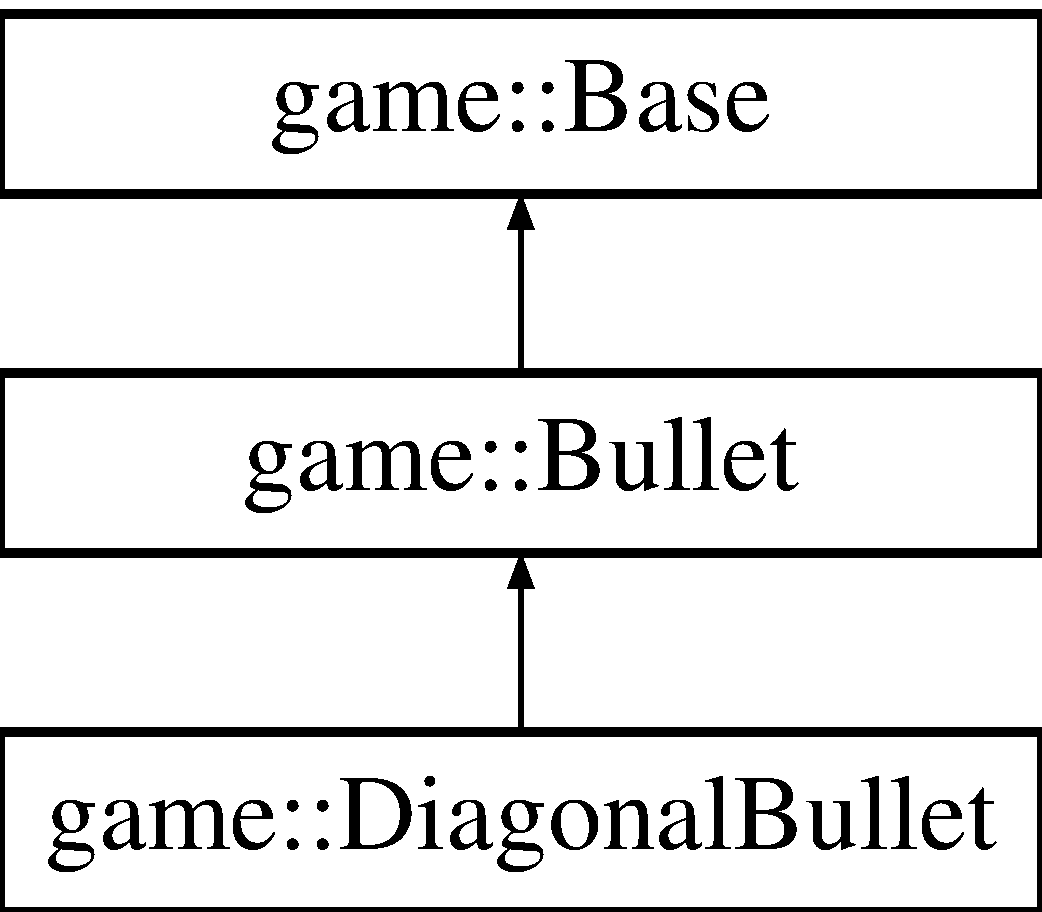
\includegraphics[height=3.000000cm]{classgame_1_1DiagonalBullet}
\end{center}
\end{figure}
\subsection*{Public Member Functions}
\begin{DoxyCompactItemize}
\item 
\mbox{\Hypertarget{classgame_1_1DiagonalBullet_a97dd705719599d66fe9b38651a3ff24c}\label{classgame_1_1DiagonalBullet_a97dd705719599d66fe9b38651a3ff24c}} 
{\bfseries Diagonal\+Bullet} (Q\+Pixmap image, int x, int y, int bullet\+\_\+velocity, bool friendly, bool right)
\item 
\mbox{\Hypertarget{classgame_1_1DiagonalBullet_aac9487bd1264212412d3217eba26287b}\label{classgame_1_1DiagonalBullet_aac9487bd1264212412d3217eba26287b}} 
void {\bfseries move} ()
\end{DoxyCompactItemize}
\subsection*{Protected Attributes}
\begin{DoxyCompactItemize}
\item 
\mbox{\Hypertarget{classgame_1_1DiagonalBullet_a72f27d077361cad14c242b74bbacb5a5}\label{classgame_1_1DiagonalBullet_a72f27d077361cad14c242b74bbacb5a5}} 
bool {\bfseries right}
\end{DoxyCompactItemize}


The documentation for this class was generated from the following files\+:\begin{DoxyCompactItemize}
\item 
diagonalbullet.\+h\item 
diagonalbullet.\+cpp\end{DoxyCompactItemize}

\hypertarget{classDialog}{}\section{Dialog Class Reference}
\label{classDialog}\index{Dialog@{Dialog}}
Inheritance diagram for Dialog\+:\begin{figure}[H]
\begin{center}
\leavevmode
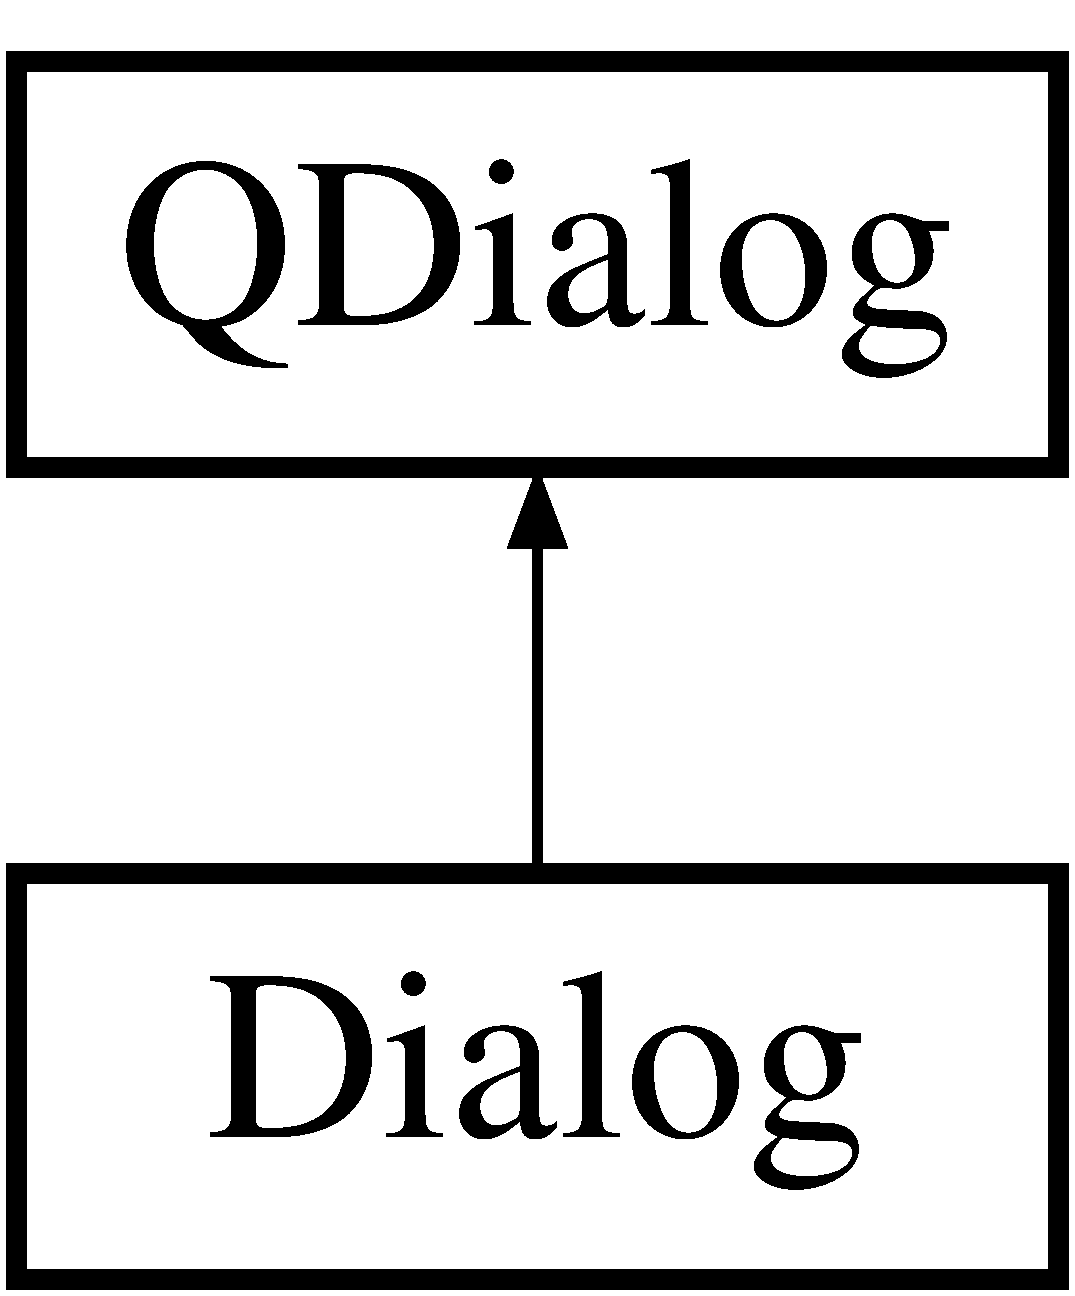
\includegraphics[height=2.000000cm]{classDialog}
\end{center}
\end{figure}
\subsection*{Public Member Functions}
\begin{DoxyCompactItemize}
\item 
\mbox{\Hypertarget{classDialog_acfa2063f9f962d394c6a645b6e7e08d8}\label{classDialog_acfa2063f9f962d394c6a645b6e7e08d8}} 
{\bfseries Dialog} (Q\+Widget $\ast$parent=0)
\end{DoxyCompactItemize}


The documentation for this class was generated from the following files\+:\begin{DoxyCompactItemize}
\item 
dialog.\+h\item 
dialog.\+cpp\end{DoxyCompactItemize}

\hypertarget{classExplosion}{}\section{Explosion Class Reference}
\label{classExplosion}\index{Explosion@{Explosion}}
\subsection*{Public Member Functions}
\begin{DoxyCompactItemize}
\item 
\mbox{\Hypertarget{classExplosion_a954e136bb5589816ca4e4d229ef5d289}\label{classExplosion_a954e136bb5589816ca4e4d229ef5d289}} 
{\bfseries Explosion} (int x, int y, int scaled\+To\+Width, Explosion\+Type type)
\item 
\mbox{\Hypertarget{classExplosion_a4d7a36e5766b1fd97767f6a45dac8965}\label{classExplosion_a4d7a36e5766b1fd97767f6a45dac8965}} 
void {\bfseries draw} (Q\+Painter $\ast$painter)
\item 
\mbox{\Hypertarget{classExplosion_ae484cce02bb4bed0d43f4078f0fb5406}\label{classExplosion_ae484cce02bb4bed0d43f4078f0fb5406}} 
void {\bfseries next\+Frame} ()
\end{DoxyCompactItemize}
\subsection*{Public Attributes}
\begin{DoxyCompactItemize}
\item 
\mbox{\Hypertarget{classExplosion_a13194cbd4c6e14352470e08960668205}\label{classExplosion_a13194cbd4c6e14352470e08960668205}} 
int {\bfseries x}
\item 
\mbox{\Hypertarget{classExplosion_a4d0073207eefaa4d8369e32ce40fbab5}\label{classExplosion_a4d0073207eefaa4d8369e32ce40fbab5}} 
int {\bfseries y}
\item 
\mbox{\Hypertarget{classExplosion_a7c4233277e796d7ec8e94dbcf981ef22}\label{classExplosion_a7c4233277e796d7ec8e94dbcf981ef22}} 
bool {\bfseries finished}
\end{DoxyCompactItemize}


The documentation for this class was generated from the following files\+:\begin{DoxyCompactItemize}
\item 
explosion.\+h\item 
explosion.\+cpp\end{DoxyCompactItemize}

\hypertarget{classgame_1_1FighterState}{}\section{game\+:\+:Fighter\+State Class Reference}
\label{classgame_1_1FighterState}\index{game\+::\+Fighter\+State@{game\+::\+Fighter\+State}}
Inheritance diagram for game\+:\+:Fighter\+State\+:\begin{figure}[H]
\begin{center}
\leavevmode
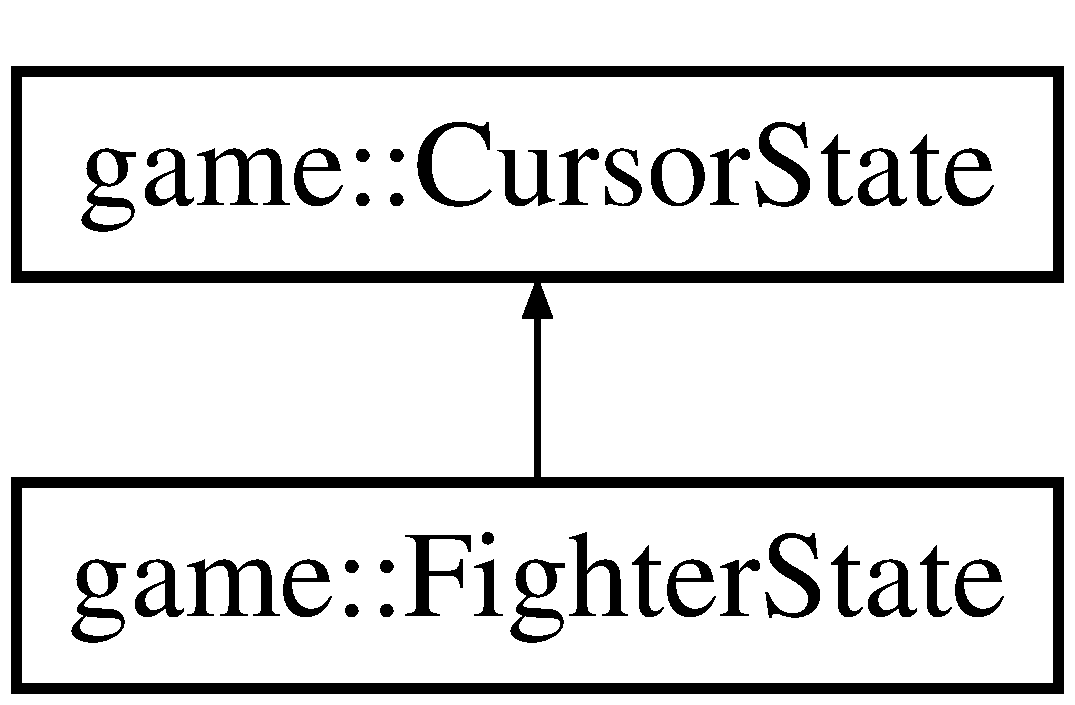
\includegraphics[height=2.000000cm]{classgame_1_1FighterState}
\end{center}
\end{figure}
\subsection*{Public Member Functions}
\begin{DoxyCompactItemize}
\item 
\mbox{\Hypertarget{classgame_1_1FighterState_ab1a6779b99bac5fd014668f2ea4b31b0}\label{classgame_1_1FighterState_ab1a6779b99bac5fd014668f2ea4b31b0}} 
{\bfseries Fighter\+State} (\hyperlink{classgame_1_1Cursor}{Cursor} $\ast$c, \hyperlink{classgame_1_1GameDialog}{Game\+Dialog} $\ast$dialog)
\item 
\mbox{\Hypertarget{classgame_1_1FighterState_a3967e2a8cef2db564707b10ce65c01a0}\label{classgame_1_1FighterState_a3967e2a8cef2db564707b10ce65c01a0}} 
void {\bfseries process\+Mouse\+Event} (Q\+Mouse\+Event $\ast$event)
\item 
\mbox{\Hypertarget{classgame_1_1FighterState_ae5450486db7312a2892b1e322ca88731}\label{classgame_1_1FighterState_ae5450486db7312a2892b1e322ca88731}} 
void {\bfseries process\+Mouse\+Press} (Q\+Mouse\+Event $\ast$event)
\item 
\mbox{\Hypertarget{classgame_1_1FighterState_acf3b706a0b2dac2a11da1e1aaa1b5ae6}\label{classgame_1_1FighterState_acf3b706a0b2dac2a11da1e1aaa1b5ae6}} 
void {\bfseries process\+Mouse\+Release} (Q\+Mouse\+Event $\ast$event)
\item 
\mbox{\Hypertarget{classgame_1_1FighterState_abdb968d67ac3918b3bec35ec3741561c}\label{classgame_1_1FighterState_abdb968d67ac3918b3bec35ec3741561c}} 
void {\bfseries update\+Cursor\+Display} ()
\item 
\mbox{\Hypertarget{classgame_1_1FighterState_aa4813a76f85bb36a4cd95eec6164cbbb}\label{classgame_1_1FighterState_aa4813a76f85bb36a4cd95eec6164cbbb}} 
void {\bfseries draw} (Q\+Painter $\ast$p)
\item 
\mbox{\Hypertarget{classgame_1_1FighterState_a38ec7475a62daf8f71d9ee78eaf0e2d3}\label{classgame_1_1FighterState_a38ec7475a62daf8f71d9ee78eaf0e2d3}} 
void {\bfseries update} ()
\item 
\mbox{\Hypertarget{classgame_1_1FighterState_a755235ed74c264900253a171d581ae1c}\label{classgame_1_1FighterState_a755235ed74c264900253a171d581ae1c}} 
void {\bfseries set\+Cursor\+Display} (bool normal)
\end{DoxyCompactItemize}
\subsection*{Additional Inherited Members}


The documentation for this class was generated from the following files\+:\begin{DoxyCompactItemize}
\item 
fighterstate.\+h\item 
fighterstate.\+cpp\end{DoxyCompactItemize}

\hypertarget{classgame_1_1GameDialog}{}\section{game\+:\+:Game\+Dialog Class Reference}
\label{classgame_1_1GameDialog}\index{game\+::\+Game\+Dialog@{game\+::\+Game\+Dialog}}
Inheritance diagram for game\+:\+:Game\+Dialog\+:\begin{figure}[H]
\begin{center}
\leavevmode
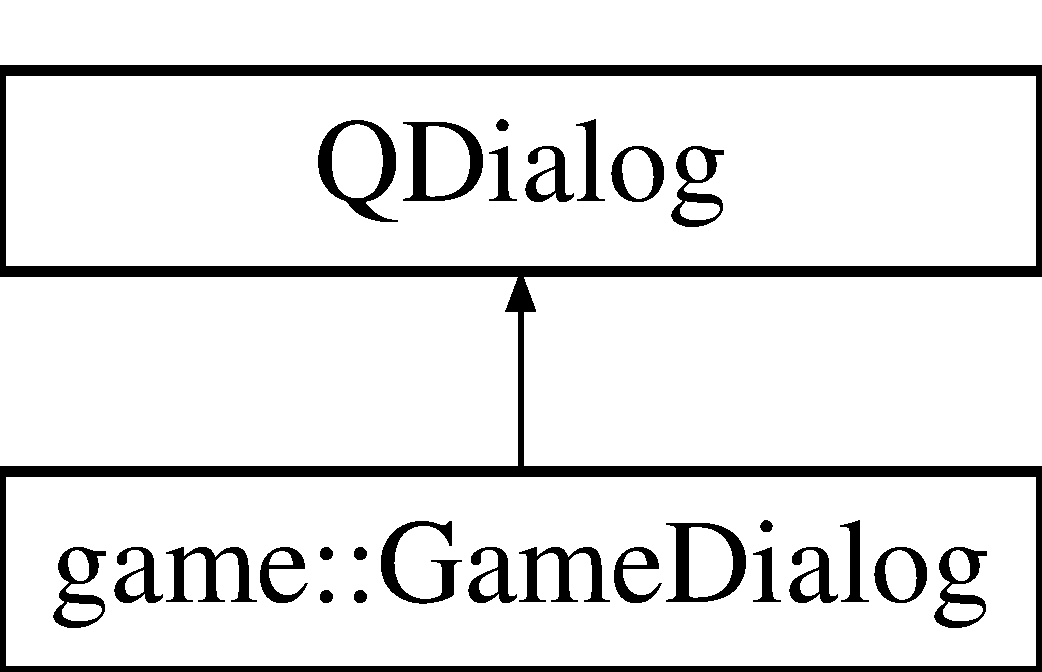
\includegraphics[height=2.000000cm]{classgame_1_1GameDialog}
\end{center}
\end{figure}
\subsection*{Public Slots}
\begin{DoxyCompactItemize}
\item 
\mbox{\Hypertarget{classgame_1_1GameDialog_a0358b408a3dea5eae10208f02b316abc}\label{classgame_1_1GameDialog_a0358b408a3dea5eae10208f02b316abc}} 
void {\bfseries next\+Frame} ()
\item 
\mbox{\Hypertarget{classgame_1_1GameDialog_ae7a5897afb7b192c1ee2346b0c523c85}\label{classgame_1_1GameDialog_ae7a5897afb7b192c1ee2346b0c523c85}} 
void {\bfseries show\+Score} ()
\end{DoxyCompactItemize}
\subsection*{Public Member Functions}
\begin{DoxyCompactItemize}
\item 
\mbox{\Hypertarget{classgame_1_1GameDialog_ada855d83e0afdf329d108f5d081f0e34}\label{classgame_1_1GameDialog_ada855d83e0afdf329d108f5d081f0e34}} 
{\bfseries Game\+Dialog} (Q\+Widget $\ast$parent=nullptr)
\item 
\mbox{\Hypertarget{classgame_1_1GameDialog_a34dffea7be3287484ba6e8d1860a6ee7}\label{classgame_1_1GameDialog_a34dffea7be3287484ba6e8d1860a6ee7}} 
void {\bfseries generate\+Aliens} (const Q\+List$<$ \hyperlink{classgame_1_1SwarmInfo}{Swarm\+Info} $>$ \&swarms)
\item 
\mbox{\Hypertarget{classgame_1_1GameDialog_a13d8b21dbfdce1364bb66c237eb69ccb}\label{classgame_1_1GameDialog_a13d8b21dbfdce1364bb66c237eb69ccb}} 
void {\bfseries paint\+Event} (Q\+Paint\+Event $\ast$event)
\item 
\mbox{\Hypertarget{classgame_1_1GameDialog_addccb9ba0f81306a68a72363c8e6bdf0}\label{classgame_1_1GameDialog_addccb9ba0f81306a68a72363c8e6bdf0}} 
void {\bfseries update\+Bullets} ()
\item 
\mbox{\Hypertarget{classgame_1_1GameDialog_af08670ba65279ac0de6f04c991b24c7b}\label{classgame_1_1GameDialog_af08670ba65279ac0de6f04c991b24c7b}} 
void {\bfseries check\+Swarm\+Collisions} (\hyperlink{classgame_1_1AlienBase}{Alien\+Base} $\ast$\&root)
\item 
\mbox{\Hypertarget{classgame_1_1GameDialog_a4e6ebb0710ca0d0814e1c615ff7f9601}\label{classgame_1_1GameDialog_a4e6ebb0710ca0d0814e1c615ff7f9601}} 
void {\bfseries request\+Name} (Q\+String info)
\item 
\mbox{\Hypertarget{classgame_1_1GameDialog_ad6d81a591bf8d475e7cdc3d628cec2bc}\label{classgame_1_1GameDialog_ad6d81a591bf8d475e7cdc3d628cec2bc}} 
void {\bfseries key\+Press\+Event} (Q\+Key\+Event $\ast$event)
\item 
\mbox{\Hypertarget{classgame_1_1GameDialog_a83f78e6ff49bcdc7e7ebd34af9bd25c9}\label{classgame_1_1GameDialog_a83f78e6ff49bcdc7e7ebd34af9bd25c9}} 
void {\bfseries key\+Release\+Event} (Q\+Key\+Event $\ast$event)
\item 
\mbox{\Hypertarget{classgame_1_1GameDialog_a7000081522bab10fed0f2b17562bdee0}\label{classgame_1_1GameDialog_a7000081522bab10fed0f2b17562bdee0}} 
void {\bfseries mouse\+Press\+Event} (Q\+Mouse\+Event $\ast$event)
\item 
\mbox{\Hypertarget{classgame_1_1GameDialog_a06136853f0dc047edd202926f5271a43}\label{classgame_1_1GameDialog_a06136853f0dc047edd202926f5271a43}} 
void {\bfseries mouse\+Release\+Event} (Q\+Mouse\+Event $\ast$event)
\item 
\mbox{\Hypertarget{classgame_1_1GameDialog_ade016d04db744346e3cc30504d9cb894}\label{classgame_1_1GameDialog_ade016d04db744346e3cc30504d9cb894}} 
void {\bfseries mouse\+Move\+Event} (Q\+Mouse\+Event $\ast$event)
\item 
\mbox{\Hypertarget{classgame_1_1GameDialog_ad039788978065d933a8c09370fc41f9b}\label{classgame_1_1GameDialog_ad039788978065d933a8c09370fc41f9b}} 
int {\bfseries get\+\_\+collided\+\_\+swarm} (\hyperlink{classgame_1_1Bullet}{Bullet} $\ast$\&b, \hyperlink{classgame_1_1AlienBase}{Alien\+Base} $\ast$\&root)
\item 
\mbox{\Hypertarget{classgame_1_1GameDialog_a15c0f76f69010da997311d3bacc544db}\label{classgame_1_1GameDialog_a15c0f76f69010da997311d3bacc544db}} 
int {\bfseries get\+\_\+collided} (\hyperlink{classgame_1_1Bullet}{Bullet} $\ast$\&b, \hyperlink{classgame_1_1AlienBase}{Alien\+Base} $\ast$\&root)
\item 
\mbox{\Hypertarget{classgame_1_1GameDialog_a72ca2411d006615c08bbd97c944fa0e9}\label{classgame_1_1GameDialog_a72ca2411d006615c08bbd97c944fa0e9}} 
void {\bfseries add\+Bullets} (const Q\+List$<$ \hyperlink{classgame_1_1Bullet}{Bullet} $\ast$$>$ \&list)
\item 
\mbox{\Hypertarget{classgame_1_1GameDialog_ac2e92dcb08b04e2855f407fa29cca007}\label{classgame_1_1GameDialog_ac2e92dcb08b04e2855f407fa29cca007}} 
int {\bfseries count\+Aliens} (\hyperlink{classgame_1_1AlienBase}{Alien\+Base} $\ast$root)
\item 
\mbox{\Hypertarget{classgame_1_1GameDialog_a3126b48b034cf10866e1c1fd5733bd6d}\label{classgame_1_1GameDialog_a3126b48b034cf10866e1c1fd5733bd6d}} 
bool {\bfseries update\+Bullets\+\_\+barrier\+Chk\+Helper} (int x, int y)
\item 
\mbox{\Hypertarget{classgame_1_1GameDialog_aaf4895fe2e8d09327eb943d0c0ad6fab}\label{classgame_1_1GameDialog_aaf4895fe2e8d09327eb943d0c0ad6fab}} 
void {\bfseries print\+Debug\+Info} (Q\+Painter $\ast$p)
\item 
\mbox{\Hypertarget{classgame_1_1GameDialog_a845533620762d3ba415bf8a1d227b755}\label{classgame_1_1GameDialog_a845533620762d3ba415bf8a1d227b755}} 
void {\bfseries init\+Commands} ()
\end{DoxyCompactItemize}
\subsection*{Static Public Member Functions}
\begin{DoxyCompactItemize}
\item 
\mbox{\Hypertarget{classgame_1_1GameDialog_ae7c1116be69edc81341379d98d3cd51d}\label{classgame_1_1GameDialog_ae7c1116be69edc81341379d98d3cd51d}} 
static int {\bfseries rand\+Int} (int low, int high)
\item 
\mbox{\Hypertarget{classgame_1_1GameDialog_a5e7a526058daf99b2b03070d255ca142}\label{classgame_1_1GameDialog_a5e7a526058daf99b2b03070d255ca142}} 
static void {\bfseries Seed\+Rand\+Int} ()
\end{DoxyCompactItemize}
\subsection*{Public Attributes}
\begin{DoxyCompactItemize}
\item 
\mbox{\Hypertarget{classgame_1_1GameDialog_a28a6eb5c4c3f7d3fea5b23b7e9de427d}\label{classgame_1_1GameDialog_a28a6eb5c4c3f7d3fea5b23b7e9de427d}} 
Q\+Timer $\ast$ {\bfseries timer}
\item 
\mbox{\Hypertarget{classgame_1_1GameDialog_a30773b8f18642c3861d29a3ad57e290e}\label{classgame_1_1GameDialog_a30773b8f18642c3861d29a3ad57e290e}} 
\hyperlink{classgame_1_1Ship}{Ship} $\ast$ {\bfseries ship}
\item 
\mbox{\Hypertarget{classgame_1_1GameDialog_ae6f27be83baf845f158789714cc2beef}\label{classgame_1_1GameDialog_ae6f27be83baf845f158789714cc2beef}} 
std\+::vector$<$ \hyperlink{classgame_1_1Bullet}{Bullet} $\ast$ $>$ {\bfseries bullets}
\item 
\mbox{\Hypertarget{classgame_1_1GameDialog_abcd0d362928cd85aba933827477fb82d}\label{classgame_1_1GameDialog_abcd0d362928cd85aba933827477fb82d}} 
\hyperlink{classgame_1_1AlienBase}{Alien\+Base} $\ast$ {\bfseries swarms}
\item 
\mbox{\Hypertarget{classgame_1_1GameDialog_a04a3af8bad4478d6c6a3e1888f32d937}\label{classgame_1_1GameDialog_a04a3af8bad4478d6c6a3e1888f32d937}} 
Q\+Sound\+Effect {\bfseries ship\+Firing\+Sound}
\item 
\mbox{\Hypertarget{classgame_1_1GameDialog_a66f5e04dea129fe0b70366aba1e2b523}\label{classgame_1_1GameDialog_a66f5e04dea129fe0b70366aba1e2b523}} 
int {\bfseries next\+\_\+instruct}
\item 
\mbox{\Hypertarget{classgame_1_1GameDialog_a1b230343b64c3abed6a00144222b9ac4}\label{classgame_1_1GameDialog_a1b230343b64c3abed6a00144222b9ac4}} 
int {\bfseries frames}
\item 
\mbox{\Hypertarget{classgame_1_1GameDialog_ab1d4c54ccb17c3adb30d9682445f5464}\label{classgame_1_1GameDialog_ab1d4c54ccb17c3adb30d9682445f5464}} 
const int {\bfseries W\+I\+D\+TH} = 800
\item 
\mbox{\Hypertarget{classgame_1_1GameDialog_aa7facc8fa930dc10444918d08ba3fd11}\label{classgame_1_1GameDialog_aa7facc8fa930dc10444918d08ba3fd11}} 
const int {\bfseries H\+E\+I\+G\+HT} = 600
\item 
\mbox{\Hypertarget{classgame_1_1GameDialog_a748f7ae8864731de8f12976b28c322ac}\label{classgame_1_1GameDialog_a748f7ae8864731de8f12976b28c322ac}} 
int {\bfseries S\+C\+A\+L\+E\+D\+W\+I\+D\+TH}
\item 
\mbox{\Hypertarget{classgame_1_1GameDialog_a79acf155e61154956908533cdf4af418}\label{classgame_1_1GameDialog_a79acf155e61154956908533cdf4af418}} 
int {\bfseries S\+C\+A\+L\+E\+D\+H\+E\+I\+G\+HT}
\item 
\mbox{\Hypertarget{classgame_1_1GameDialog_aa8ff1457afd4b17328365ae03d8d9cfa}\label{classgame_1_1GameDialog_aa8ff1457afd4b17328365ae03d8d9cfa}} 
int {\bfseries S\+T\+A\+T\+U\+S\+B\+A\+R\+H\+E\+I\+G\+HT}
\item 
\mbox{\Hypertarget{classgame_1_1GameDialog_aa8d925783a0af1b9986c676c5a309380}\label{classgame_1_1GameDialog_aa8d925783a0af1b9986c676c5a309380}} 
bool {\bfseries paused}
\item 
\mbox{\Hypertarget{classgame_1_1GameDialog_adbb0cec124eb76fc7427a0ffa5522427}\label{classgame_1_1GameDialog_adbb0cec124eb76fc7427a0ffa5522427}} 
\hyperlink{classgame_1_1Menu}{Menu} $\ast$ {\bfseries menu}
\item 
\mbox{\Hypertarget{classgame_1_1GameDialog_a74a29f926edd81e1375649cd9d3ed89f}\label{classgame_1_1GameDialog_a74a29f926edd81e1375649cd9d3ed89f}} 
\hyperlink{classgame_1_1StageMaker}{Stage\+Maker} {\bfseries stage\+Maker}
\item 
\mbox{\Hypertarget{classgame_1_1GameDialog_a868f1ba64723e6baa8ef359ac73f9264}\label{classgame_1_1GameDialog_a868f1ba64723e6baa8ef359ac73f9264}} 
bool {\bfseries debug\+Mode}
\item 
\mbox{\Hypertarget{classgame_1_1GameDialog_a8a34cb2e9876b951153069a5cb87e1fb}\label{classgame_1_1GameDialog_a8a34cb2e9876b951153069a5cb87e1fb}} 
double {\bfseries timer\+Modifier}
\item 
\mbox{\Hypertarget{classgame_1_1GameDialog_ab118adae88976a3d0977501692dcf498}\label{classgame_1_1GameDialog_ab118adae88976a3d0977501692dcf498}} 
int {\bfseries power\+Up\+Drop\+Rate}
\item 
\mbox{\Hypertarget{classgame_1_1GameDialog_aeba26be6d4fce4c16078b18e9eb355fd}\label{classgame_1_1GameDialog_aeba26be6d4fce4c16078b18e9eb355fd}} 
int {\bfseries game\+Score}
\item 
\mbox{\Hypertarget{classgame_1_1GameDialog_a80cd1beeb3655d5767e4bfd67cee843f}\label{classgame_1_1GameDialog_a80cd1beeb3655d5767e4bfd67cee843f}} 
bool {\bfseries legacy\+Mode}
\item 
\mbox{\Hypertarget{classgame_1_1GameDialog_afac4c3fff6fcd12e60052c4fed527531}\label{classgame_1_1GameDialog_afac4c3fff6fcd12e60052c4fed527531}} 
int {\bfseries cur\+Stage\+Num}
\item 
\mbox{\Hypertarget{classgame_1_1GameDialog_a4711f2a9c4ef0424d31bfc824becf134}\label{classgame_1_1GameDialog_a4711f2a9c4ef0424d31bfc824becf134}} 
Q\+Rect {\bfseries stage\+Transition\+Box}
\item 
\mbox{\Hypertarget{classgame_1_1GameDialog_a898b490cecdc8c0638333e1d40174755}\label{classgame_1_1GameDialog_a898b490cecdc8c0638333e1d40174755}} 
bool {\bfseries stage\+Transition}
\item 
\mbox{\Hypertarget{classgame_1_1GameDialog_a1f4332f40d03e76fcbb2b1a92d8577ed}\label{classgame_1_1GameDialog_a1f4332f40d03e76fcbb2b1a92d8577ed}} 
std\+::vector$<$ \hyperlink{classExplosion}{Explosion} $>$ {\bfseries explosions}
\item 
\mbox{\Hypertarget{classgame_1_1GameDialog_a09bf5d984d42869d05e2d3cc7463779c}\label{classgame_1_1GameDialog_a09bf5d984d42869d05e2d3cc7463779c}} 
std\+::vector$<$ \hyperlink{classgame_1_1BarrierBlock}{Barrier\+Block} $>$ {\bfseries barriers}
\item 
\mbox{\Hypertarget{classgame_1_1GameDialog_ac0af6b65ee7430b3037f8e8df854a2a2}\label{classgame_1_1GameDialog_ac0af6b65ee7430b3037f8e8df854a2a2}} 
std\+::vector$<$ \hyperlink{classgame_1_1Powerup}{Powerup} $>$ {\bfseries powerups}
\item 
\mbox{\Hypertarget{classgame_1_1GameDialog_afba06639685f064a60e8a5dada570e8c}\label{classgame_1_1GameDialog_afba06639685f064a60e8a5dada570e8c}} 
\hyperlink{structgame_1_1LaserBeam}{Laser\+Beam} {\bfseries laser\+Beam}
\item 
\mbox{\Hypertarget{classgame_1_1GameDialog_a3ca7bf0ecb861fa938fa3de7dc3acc7a}\label{classgame_1_1GameDialog_a3ca7bf0ecb861fa938fa3de7dc3acc7a}} 
\hyperlink{classgame_1_1StatusBar}{Status\+Bar} {\bfseries status\+Bar}
\item 
\mbox{\Hypertarget{classgame_1_1GameDialog_a17d93b8febe2eec1522208ad92daba93}\label{classgame_1_1GameDialog_a17d93b8febe2eec1522208ad92daba93}} 
\hyperlink{classgame_1_1Config}{Config} $\ast$ {\bfseries c}
\item 
\mbox{\Hypertarget{classgame_1_1GameDialog_a2e4a03e762401ff2248aced6d02a3b9c}\label{classgame_1_1GameDialog_a2e4a03e762401ff2248aced6d02a3b9c}} 
\hyperlink{classgame_1_1LeaderBoard}{Leader\+Board} {\bfseries leader\+Board}
\item 
\mbox{\Hypertarget{classgame_1_1GameDialog_a0db0d5e61c261d8cdf4335c5c5e4a7be}\label{classgame_1_1GameDialog_a0db0d5e61c261d8cdf4335c5c5e4a7be}} 
\hyperlink{classgame_1_1GameMenu}{Game\+Menu} {\bfseries game\+Menu}
\item 
\mbox{\Hypertarget{classgame_1_1GameDialog_a268c70040a5990c8aec70a2d93daa7d4}\label{classgame_1_1GameDialog_a268c70040a5990c8aec70a2d93daa7d4}} 
\hyperlink{classLeaderBoardNameRequest}{Leader\+Board\+Name\+Request} {\bfseries leader\+Board\+Name\+Request}
\item 
\mbox{\Hypertarget{classgame_1_1GameDialog_a62a4c0f4a728439f53886e362e3d15fe}\label{classgame_1_1GameDialog_a62a4c0f4a728439f53886e362e3d15fe}} 
bool {\bfseries player\+Override}
\item 
\mbox{\Hypertarget{classgame_1_1GameDialog_af0e8d1e789c9552cdc0f6a9f2dcd9e3c}\label{classgame_1_1GameDialog_af0e8d1e789c9552cdc0f6a9f2dcd9e3c}} 
std\+::map$<$ int, bool $>$ {\bfseries pressed\+Keys}
\item 
\mbox{\Hypertarget{classgame_1_1GameDialog_ac09d774d45ee879bfca90eac89da3c9a}\label{classgame_1_1GameDialog_ac09d774d45ee879bfca90eac89da3c9a}} 
\hyperlink{classBackground}{Background} {\bfseries bg}
\item 
\mbox{\Hypertarget{classgame_1_1GameDialog_a3dd11135d6ac99dfb335d0d025749b4b}\label{classgame_1_1GameDialog_a3dd11135d6ac99dfb335d0d025749b4b}} 
\hyperlink{classgame_1_1Cursor}{Cursor} {\bfseries cursor}
\item 
\mbox{\Hypertarget{classgame_1_1GameDialog_a6d69c03e37c7ee1c7ad3daf0eed9d43a}\label{classgame_1_1GameDialog_a6d69c03e37c7ee1c7ad3daf0eed9d43a}} 
G\+A\+M\+E\+\_\+\+S\+T\+A\+T\+US {\bfseries current\+State}
\item 
\mbox{\Hypertarget{classgame_1_1GameDialog_a26efb707880bdbf7b0b40a2b4de7a655}\label{classgame_1_1GameDialog_a26efb707880bdbf7b0b40a2b4de7a655}} 
std\+::unique\+\_\+ptr$<$ \hyperlink{classgame_1_1Command}{Command} $>$ {\bfseries command\+Game\+Start}
\item 
\mbox{\Hypertarget{classgame_1_1GameDialog_a04258fc97d042e928b85bb4b24e784c4}\label{classgame_1_1GameDialog_a04258fc97d042e928b85bb4b24e784c4}} 
std\+::unique\+\_\+ptr$<$ \hyperlink{classgame_1_1Command}{Command} $>$ {\bfseries command\+Game\+Pause}
\item 
\mbox{\Hypertarget{classgame_1_1GameDialog_aa196c8f6fbd53eed98995d67a2f7be2b}\label{classgame_1_1GameDialog_aa196c8f6fbd53eed98995d67a2f7be2b}} 
std\+::unique\+\_\+ptr$<$ \hyperlink{classgame_1_1Command}{Command} $>$ {\bfseries command\+Clear\+Stage}
\item 
\mbox{\Hypertarget{classgame_1_1GameDialog_a4212aff142abec8287e3a555e9f137b1}\label{classgame_1_1GameDialog_a4212aff142abec8287e3a555e9f137b1}} 
std\+::unique\+\_\+ptr$<$ \hyperlink{classgame_1_1Command}{Command} $>$ {\bfseries command\+Restart\+Stage}
\item 
\mbox{\Hypertarget{classgame_1_1GameDialog_a101ef135dbda9b8ca105ad3483eeaa93}\label{classgame_1_1GameDialog_a101ef135dbda9b8ca105ad3483eeaa93}} 
std\+::unique\+\_\+ptr$<$ \hyperlink{classgame_1_1Command}{Command} $>$ {\bfseries command\+Go\+To\+Title\+Screen\+Mode}
\item 
\mbox{\Hypertarget{classgame_1_1GameDialog_aad3827dadd16093327a16240f4ded2e1}\label{classgame_1_1GameDialog_aad3827dadd16093327a16240f4ded2e1}} 
std\+::unique\+\_\+ptr$<$ \hyperlink{classgame_1_1Command}{Command} $>$ {\bfseries command\+Go\+To\+Game\+Mode}
\item 
\mbox{\Hypertarget{classgame_1_1GameDialog_a3baffe837701cda101f8242d1f94d01a}\label{classgame_1_1GameDialog_a3baffe837701cda101f8242d1f94d01a}} 
std\+::unique\+\_\+ptr$<$ \hyperlink{classgame_1_1Command}{Command} $>$ {\bfseries command\+Go\+To\+Stage\+Maker\+Mode}
\item 
\mbox{\Hypertarget{classgame_1_1GameDialog_af909896fedcf53d1b1343d0b262af592}\label{classgame_1_1GameDialog_af909896fedcf53d1b1343d0b262af592}} 
std\+::unique\+\_\+ptr$<$ \hyperlink{classgame_1_1Command}{Command} $>$ {\bfseries command\+Go\+To\+Leader\+Board\+Mode}
\end{DoxyCompactItemize}


The documentation for this class was generated from the following files\+:\begin{DoxyCompactItemize}
\item 
gamedialog.\+h\item 
gamedialog.\+cpp\end{DoxyCompactItemize}

\hypertarget{classgame_1_1GameMenu}{}\section{game\+:\+:Game\+Menu Class Reference}
\label{classgame_1_1GameMenu}\index{game\+::\+Game\+Menu@{game\+::\+Game\+Menu}}
Inheritance diagram for game\+:\+:Game\+Menu\+:\begin{figure}[H]
\begin{center}
\leavevmode
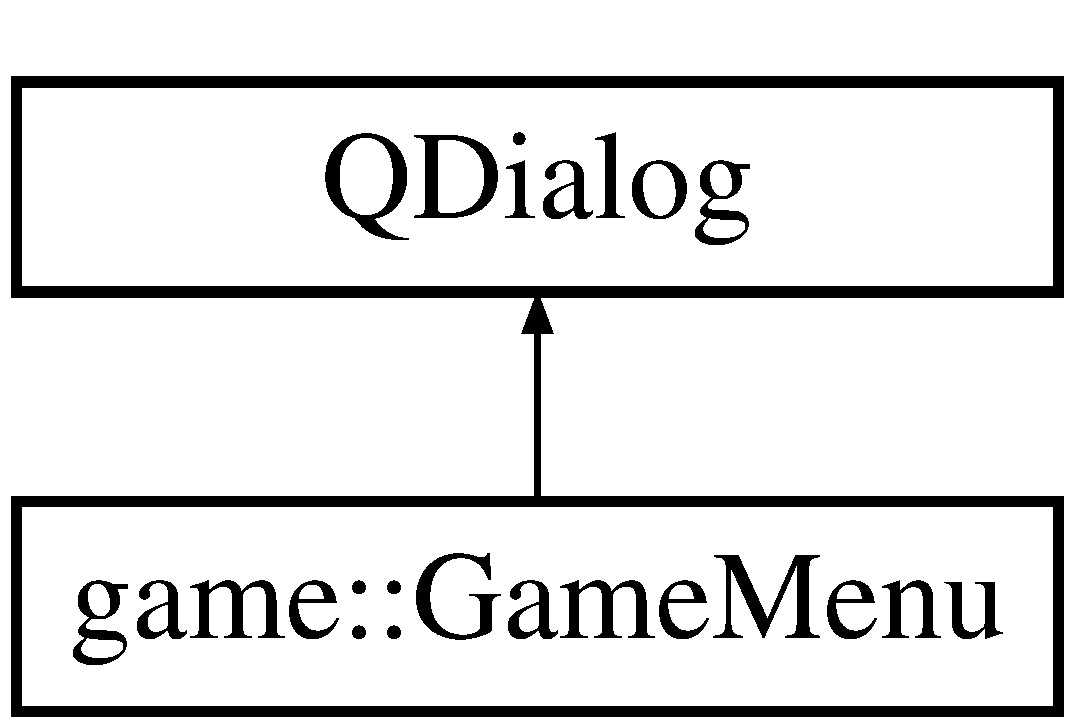
\includegraphics[height=2.000000cm]{classgame_1_1GameMenu}
\end{center}
\end{figure}
\subsection*{Public Member Functions}
\begin{DoxyCompactItemize}
\item 
\mbox{\Hypertarget{classgame_1_1GameMenu_aeca8d3ef148f8a7aef0748d6c7294ead}\label{classgame_1_1GameMenu_aeca8d3ef148f8a7aef0748d6c7294ead}} 
{\bfseries Game\+Menu} (\hyperlink{classgame_1_1GameDialog}{Game\+Dialog} $\ast$g\+Dialog, Q\+Widget $\ast$parent=0)
\end{DoxyCompactItemize}
\subsection*{Public Attributes}
\begin{DoxyCompactItemize}
\item 
\mbox{\Hypertarget{classgame_1_1GameMenu_a58ed39bf95b0b3b081aafa8ca0f80664}\label{classgame_1_1GameMenu_a58ed39bf95b0b3b081aafa8ca0f80664}} 
Ui\+::\+Game\+Menu $\ast$ {\bfseries ui}
\end{DoxyCompactItemize}


The documentation for this class was generated from the following files\+:\begin{DoxyCompactItemize}
\item 
gamemenu.\+h\item 
gamemenu.\+cpp\end{DoxyCompactItemize}

\hypertarget{classgame_1_1Hunter}{}\section{game\+:\+:Hunter Class Reference}
\label{classgame_1_1Hunter}\index{game\+::\+Hunter@{game\+::\+Hunter}}
Inheritance diagram for game\+:\+:Hunter\+:\begin{figure}[H]
\begin{center}
\leavevmode
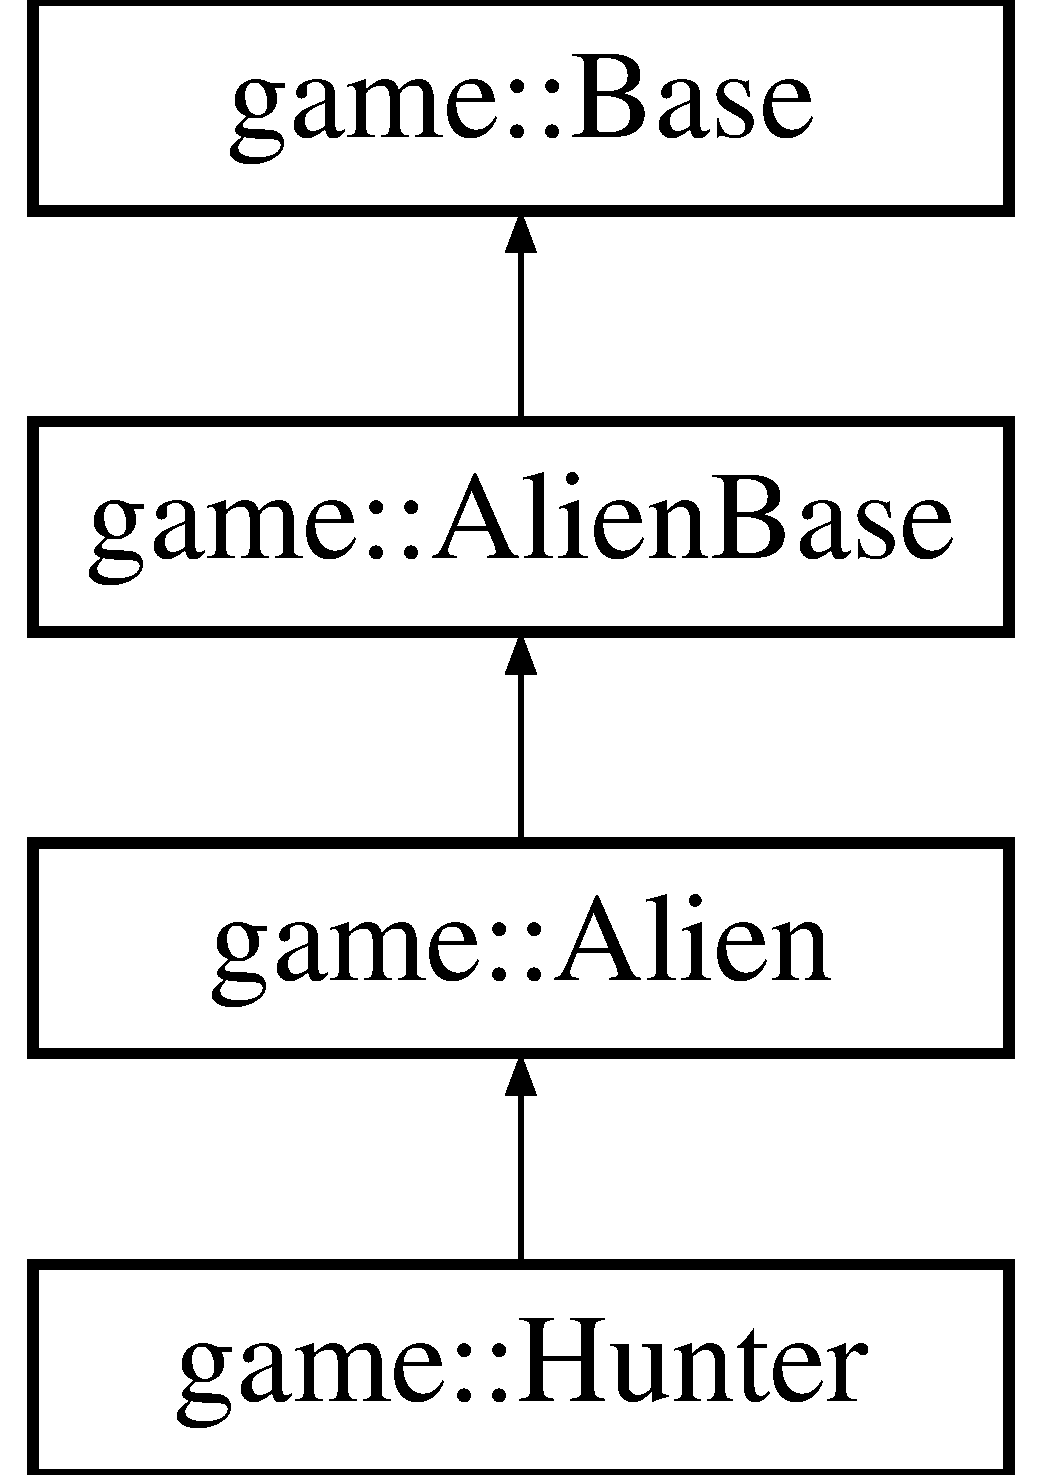
\includegraphics[height=4.000000cm]{classgame_1_1Hunter}
\end{center}
\end{figure}
\subsection*{Public Member Functions}
\begin{DoxyCompactItemize}
\item 
\mbox{\Hypertarget{classgame_1_1Hunter_a5f9f59105e5a25f0a6b2f936737f3a10}\label{classgame_1_1Hunter_a5f9f59105e5a25f0a6b2f936737f3a10}} 
{\bfseries Hunter} (Q\+Pixmap image, int x, int y, int velocity, int score, Q\+String base\+Type, \hyperlink{classgame_1_1Base}{Base} \&ship, int stray)
\item 
\mbox{\Hypertarget{classgame_1_1Hunter_ad0ac31a35cccc2a70481eccad2c10e3a}\label{classgame_1_1Hunter_ad0ac31a35cccc2a70481eccad2c10e3a}} 
void {\bfseries move} (Q\+String direction)
\item 
\mbox{\Hypertarget{classgame_1_1Hunter_a955e3e965209e19256100b3602c3d158}\label{classgame_1_1Hunter_a955e3e965209e19256100b3602c3d158}} 
Q\+List$<$ \hyperlink{classgame_1_1Bullet}{Bullet} $\ast$ $>$ {\bfseries shoot} (Q\+String type)
\item 
\mbox{\Hypertarget{classgame_1_1Hunter_af22d5de5a6fc86ae60190aabf3922064}\label{classgame_1_1Hunter_af22d5de5a6fc86ae60190aabf3922064}} 
Q\+List$<$ \hyperlink{classgame_1_1Bullet}{Bullet} $\ast$ $>$ {\bfseries react} ()
\end{DoxyCompactItemize}
\subsection*{Protected Member Functions}
\begin{DoxyCompactItemize}
\item 
\mbox{\Hypertarget{classgame_1_1Hunter_a0f2031907aed40e5b6da9f329ac42b11}\label{classgame_1_1Hunter_a0f2031907aed40e5b6da9f329ac42b11}} 
Q\+String {\bfseries calculate\+Direction} ()
\end{DoxyCompactItemize}
\subsection*{Protected Attributes}
\begin{DoxyCompactItemize}
\item 
\mbox{\Hypertarget{classgame_1_1Hunter_ab3891c72a1f10574fa959eac73e776d1}\label{classgame_1_1Hunter_ab3891c72a1f10574fa959eac73e776d1}} 
int {\bfseries stray}
\item 
\mbox{\Hypertarget{classgame_1_1Hunter_a4ede49f4343fa2023af16eb70b320f8f}\label{classgame_1_1Hunter_a4ede49f4343fa2023af16eb70b320f8f}} 
\hyperlink{classgame_1_1Base}{Base} \& {\bfseries ship}
\item 
\mbox{\Hypertarget{classgame_1_1Hunter_a73f0f5f7a2817ae1078613a4a045fe91}\label{classgame_1_1Hunter_a73f0f5f7a2817ae1078613a4a045fe91}} 
Q\+String {\bfseries base\+Type}
\end{DoxyCompactItemize}


The documentation for this class was generated from the following files\+:\begin{DoxyCompactItemize}
\item 
hunter.\+h\item 
hunter.\+cpp\end{DoxyCompactItemize}

\hypertarget{classgame_1_1InstructionRequest}{}\section{game\+:\+:Instruction\+Request Class Reference}
\label{classgame_1_1InstructionRequest}\index{game\+::\+Instruction\+Request@{game\+::\+Instruction\+Request}}
Inheritance diagram for game\+:\+:Instruction\+Request\+:\begin{figure}[H]
\begin{center}
\leavevmode
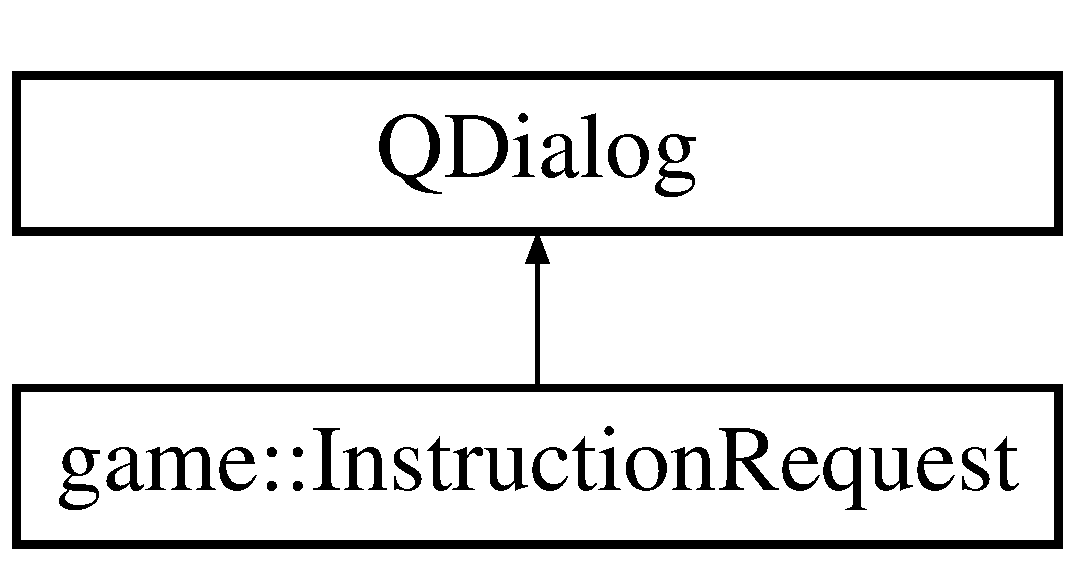
\includegraphics[height=2.000000cm]{classgame_1_1InstructionRequest}
\end{center}
\end{figure}
\subsection*{Public Member Functions}
\begin{DoxyCompactItemize}
\item 
\mbox{\Hypertarget{classgame_1_1InstructionRequest_a791e508bd6068b6bd703fd3f9782271f}\label{classgame_1_1InstructionRequest_a791e508bd6068b6bd703fd3f9782271f}} 
{\bfseries Instruction\+Request} (Q\+Widget $\ast$parent=0)
\end{DoxyCompactItemize}
\subsection*{Public Attributes}
\begin{DoxyCompactItemize}
\item 
\mbox{\Hypertarget{classgame_1_1InstructionRequest_ab2d24dd114d756dad37921ef4dcfc662}\label{classgame_1_1InstructionRequest_ab2d24dd114d756dad37921ef4dcfc662}} 
Q\+String {\bfseries instructions}
\item 
\mbox{\Hypertarget{classgame_1_1InstructionRequest_abb5c66025d6efc5921cbb1e74b2f7870}\label{classgame_1_1InstructionRequest_abb5c66025d6efc5921cbb1e74b2f7870}} 
\hyperlink{structgame_1_1SMakerPlacedObject}{S\+Maker\+Placed\+Object} $\ast$ {\bfseries instruction\+Box}
\end{DoxyCompactItemize}


The documentation for this class was generated from the following files\+:\begin{DoxyCompactItemize}
\item 
instructionirequest.\+h\item 
instructionirequest.\+cpp\end{DoxyCompactItemize}

\hypertarget{structgame_1_1LaserBeam}{}\section{game\+:\+:Laser\+Beam Struct Reference}
\label{structgame_1_1LaserBeam}\index{game\+::\+Laser\+Beam@{game\+::\+Laser\+Beam}}
\subsection*{Public Attributes}
\begin{DoxyCompactItemize}
\item 
\mbox{\Hypertarget{structgame_1_1LaserBeam_a27e1508dcb195c54d04747a7549a1186}\label{structgame_1_1LaserBeam_a27e1508dcb195c54d04747a7549a1186}} 
int {\bfseries originX}
\item 
\mbox{\Hypertarget{structgame_1_1LaserBeam_ade2146adfea9744f171c6882a4f36b8d}\label{structgame_1_1LaserBeam_ade2146adfea9744f171c6882a4f36b8d}} 
int {\bfseries originY}
\item 
\mbox{\Hypertarget{structgame_1_1LaserBeam_a57902395c0955a1432a8ca35f3a79e74}\label{structgame_1_1LaserBeam_a57902395c0955a1432a8ca35f3a79e74}} 
int {\bfseries width}
\item 
\mbox{\Hypertarget{structgame_1_1LaserBeam_a40211d9aacb82d8aa4fec703b54b56cb}\label{structgame_1_1LaserBeam_a40211d9aacb82d8aa4fec703b54b56cb}} 
bool {\bfseries exists}
\end{DoxyCompactItemize}


The documentation for this struct was generated from the following file\+:\begin{DoxyCompactItemize}
\item 
bullet.\+h\end{DoxyCompactItemize}

\hypertarget{classgame_1_1LeaderBoard}{}\section{game\+:\+:Leader\+Board Class Reference}
\label{classgame_1_1LeaderBoard}\index{game\+::\+Leader\+Board@{game\+::\+Leader\+Board}}
\subsection*{Public Member Functions}
\begin{DoxyCompactItemize}
\item 
\mbox{\Hypertarget{classgame_1_1LeaderBoard_ad1a3f902ecb6ae0f0eeb6134e8b308c4}\label{classgame_1_1LeaderBoard_ad1a3f902ecb6ae0f0eeb6134e8b308c4}} 
void {\bfseries init} (int Screen\+Width, int Screen\+Height, Q\+String filename)
\item 
\mbox{\Hypertarget{classgame_1_1LeaderBoard_accfa2beee9cff36f68bbdf1b3c28ac24}\label{classgame_1_1LeaderBoard_accfa2beee9cff36f68bbdf1b3c28ac24}} 
void {\bfseries draw} (Q\+Painter $\ast$p)
\item 
\mbox{\Hypertarget{classgame_1_1LeaderBoard_addaa59c4c16508eaeedeb7ffc4d29d4e}\label{classgame_1_1LeaderBoard_addaa59c4c16508eaeedeb7ffc4d29d4e}} 
void {\bfseries update} ()
\item 
\mbox{\Hypertarget{classgame_1_1LeaderBoard_ad7b3050c23063ce16a28e13dbfda3c92}\label{classgame_1_1LeaderBoard_ad7b3050c23063ce16a28e13dbfda3c92}} 
void {\bfseries reset} ()
\end{DoxyCompactItemize}
\subsection*{Public Attributes}
\begin{DoxyCompactItemize}
\item 
\mbox{\Hypertarget{classgame_1_1LeaderBoard_aeedce6fae97cb0d4cf4eb3ac38fbd52d}\label{classgame_1_1LeaderBoard_aeedce6fae97cb0d4cf4eb3ac38fbd52d}} 
Q\+Rect {\bfseries leader\+Board\+Title}
\item 
\mbox{\Hypertarget{classgame_1_1LeaderBoard_a5344e2bd9bef8382d7813a59c079e906}\label{classgame_1_1LeaderBoard_a5344e2bd9bef8382d7813a59c079e906}} 
std\+::vector$<$ std\+::pair$<$ Q\+Rect, Q\+String\+List $>$ $>$ {\bfseries players}
\item 
\mbox{\Hypertarget{classgame_1_1LeaderBoard_a3b2e1276e2c1f85c9ef23dd3a3e8a6d5}\label{classgame_1_1LeaderBoard_a3b2e1276e2c1f85c9ef23dd3a3e8a6d5}} 
bool {\bfseries finished}
\item 
\mbox{\Hypertarget{classgame_1_1LeaderBoard_a84e82723cdcf2cacf5a025b7f6319f28}\label{classgame_1_1LeaderBoard_a84e82723cdcf2cacf5a025b7f6319f28}} 
Q\+String {\bfseries filename}
\item 
\mbox{\Hypertarget{classgame_1_1LeaderBoard_afa1d1955f9d68682da69c4376523d370}\label{classgame_1_1LeaderBoard_afa1d1955f9d68682da69c4376523d370}} 
int {\bfseries Screen\+Width}
\item 
\mbox{\Hypertarget{classgame_1_1LeaderBoard_a1b601724e64b94e54374ae7fe657bd31}\label{classgame_1_1LeaderBoard_a1b601724e64b94e54374ae7fe657bd31}} 
int {\bfseries Screen\+Height}
\end{DoxyCompactItemize}


The documentation for this class was generated from the following files\+:\begin{DoxyCompactItemize}
\item 
leaderboard.\+h\item 
leaderboard.\+cpp\end{DoxyCompactItemize}

\hypertarget{classLeaderBoardNameRequest}{}\section{Leader\+Board\+Name\+Request Class Reference}
\label{classLeaderBoardNameRequest}\index{Leader\+Board\+Name\+Request@{Leader\+Board\+Name\+Request}}
Inheritance diagram for Leader\+Board\+Name\+Request\+:\begin{figure}[H]
\begin{center}
\leavevmode
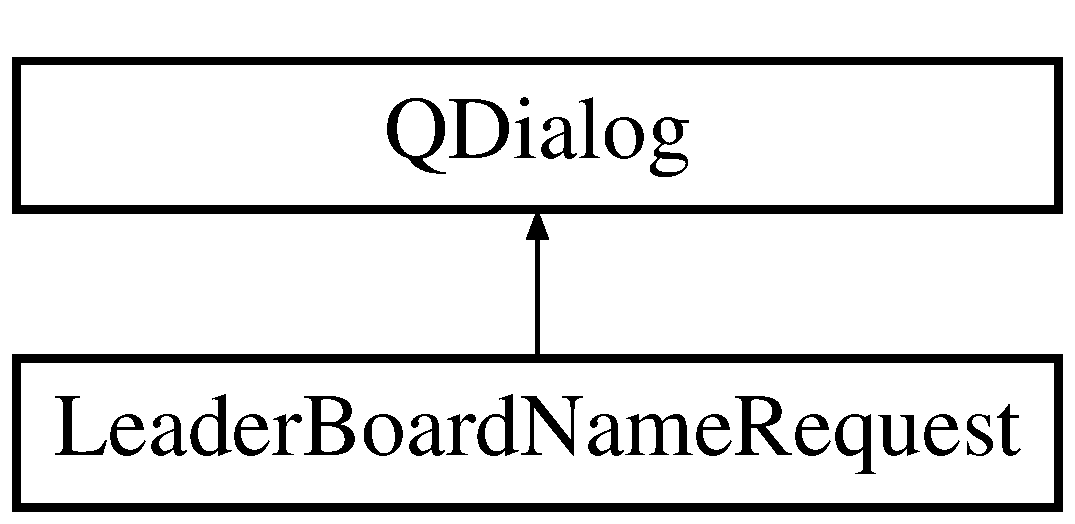
\includegraphics[height=2.000000cm]{classLeaderBoardNameRequest}
\end{center}
\end{figure}
\subsection*{Public Member Functions}
\begin{DoxyCompactItemize}
\item 
\mbox{\Hypertarget{classLeaderBoardNameRequest_a83512d43005fcfb7cdc737b99e1f8759}\label{classLeaderBoardNameRequest_a83512d43005fcfb7cdc737b99e1f8759}} 
{\bfseries Leader\+Board\+Name\+Request} (Q\+String filename, \hyperlink{classgame_1_1GameDialog}{game\+::\+Game\+Dialog} $\ast$g\+Dialog, Q\+Widget $\ast$parent=0)
\end{DoxyCompactItemize}
\subsection*{Public Attributes}
\begin{DoxyCompactItemize}
\item 
\mbox{\Hypertarget{classLeaderBoardNameRequest_a9585af9622650e407cf80de992180d23}\label{classLeaderBoardNameRequest_a9585af9622650e407cf80de992180d23}} 
Ui\+::leader\+Board\+Name\+Request $\ast$ {\bfseries ui}
\item 
\mbox{\Hypertarget{classLeaderBoardNameRequest_afce5bd688f07e991a03ba05390fa787f}\label{classLeaderBoardNameRequest_afce5bd688f07e991a03ba05390fa787f}} 
Q\+String {\bfseries filename}
\item 
\mbox{\Hypertarget{classLeaderBoardNameRequest_a3b14b1142491e1b98f9c7267b79a8c86}\label{classLeaderBoardNameRequest_a3b14b1142491e1b98f9c7267b79a8c86}} 
\hyperlink{classgame_1_1GameDialog}{game\+::\+Game\+Dialog} $\ast$ {\bfseries g\+Dialog}
\end{DoxyCompactItemize}


The documentation for this class was generated from the following files\+:\begin{DoxyCompactItemize}
\item 
leaderboardnamerequest.\+h\item 
leaderboardnamerequest.\+cpp\end{DoxyCompactItemize}

\hypertarget{classgame_1_1MakerState}{}\section{game\+:\+:Maker\+State Class Reference}
\label{classgame_1_1MakerState}\index{game\+::\+Maker\+State@{game\+::\+Maker\+State}}
Inheritance diagram for game\+:\+:Maker\+State\+:\begin{figure}[H]
\begin{center}
\leavevmode
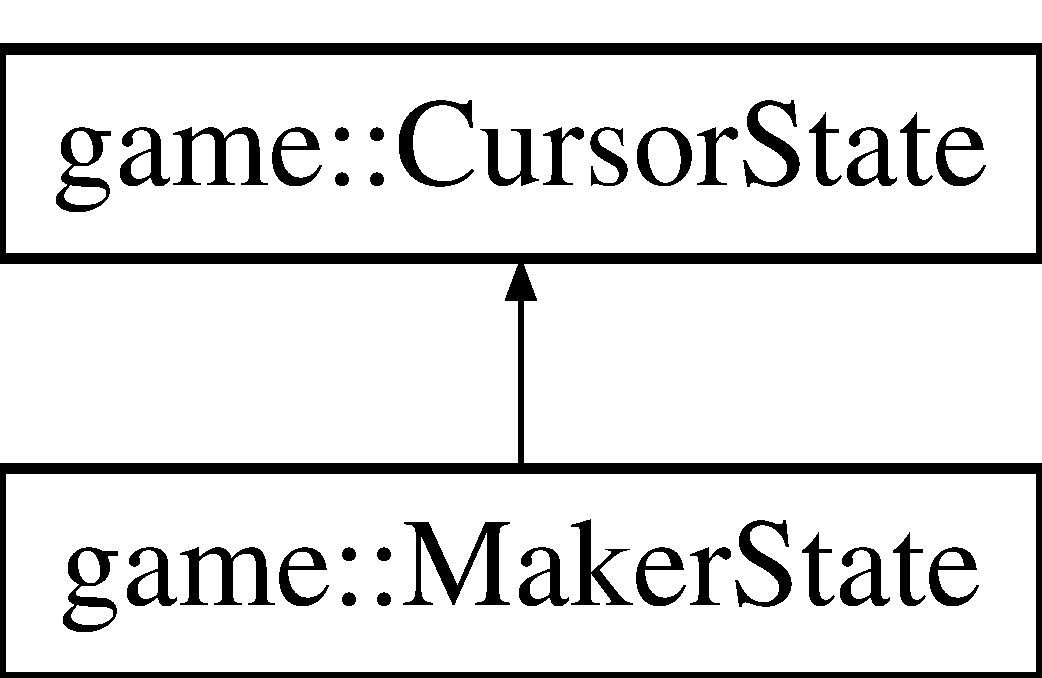
\includegraphics[height=2.000000cm]{classgame_1_1MakerState}
\end{center}
\end{figure}
\subsection*{Public Member Functions}
\begin{DoxyCompactItemize}
\item 
\mbox{\Hypertarget{classgame_1_1MakerState_a821b031d287b7602f7d6eff6b8fb9162}\label{classgame_1_1MakerState_a821b031d287b7602f7d6eff6b8fb9162}} 
{\bfseries Maker\+State} (\hyperlink{classgame_1_1Cursor}{Cursor} $\ast$c, \hyperlink{classgame_1_1GameDialog}{Game\+Dialog} $\ast$dialog)
\item 
\mbox{\Hypertarget{classgame_1_1MakerState_a772ef3b0af5a00093b8270ae3a3dc9eb}\label{classgame_1_1MakerState_a772ef3b0af5a00093b8270ae3a3dc9eb}} 
void {\bfseries process\+Mouse\+Event} (Q\+Mouse\+Event $\ast$event)
\item 
\mbox{\Hypertarget{classgame_1_1MakerState_a7233722c5ba24ebc1c0e0d74930a7920}\label{classgame_1_1MakerState_a7233722c5ba24ebc1c0e0d74930a7920}} 
void {\bfseries process\+Mouse\+Press} (Q\+Mouse\+Event $\ast$event)
\item 
\mbox{\Hypertarget{classgame_1_1MakerState_a526d7ce9ce017fbbc279ba08217dc9cd}\label{classgame_1_1MakerState_a526d7ce9ce017fbbc279ba08217dc9cd}} 
void {\bfseries process\+Mouse\+Release} (Q\+Mouse\+Event $\ast$event)
\item 
\mbox{\Hypertarget{classgame_1_1MakerState_ae89465bddd33a4c11b6ae31a6f58b66d}\label{classgame_1_1MakerState_ae89465bddd33a4c11b6ae31a6f58b66d}} 
void {\bfseries update\+Cursor\+Display} ()
\item 
\mbox{\Hypertarget{classgame_1_1MakerState_a88bf5ae574e0e79ec78ec890f46738e8}\label{classgame_1_1MakerState_a88bf5ae574e0e79ec78ec890f46738e8}} 
void {\bfseries draw} (Q\+Painter $\ast$p)
\item 
\mbox{\Hypertarget{classgame_1_1MakerState_aa61fa26dd0c3fbe35b1f7f7f4579a1f1}\label{classgame_1_1MakerState_aa61fa26dd0c3fbe35b1f7f7f4579a1f1}} 
void {\bfseries update} ()
\end{DoxyCompactItemize}
\subsection*{Additional Inherited Members}


The documentation for this class was generated from the following files\+:\begin{DoxyCompactItemize}
\item 
makerstate.\+h\item 
makerstate.\+cpp\end{DoxyCompactItemize}

\hypertarget{classgame_1_1Menu}{}\section{game\+:\+:Menu Class Reference}
\label{classgame_1_1Menu}\index{game\+::\+Menu@{game\+::\+Menu}}
\subsection*{Public Member Functions}
\begin{DoxyCompactItemize}
\item 
\mbox{\Hypertarget{classgame_1_1Menu_aeac4e21eb63e4279fb241607043a58da}\label{classgame_1_1Menu_aeac4e21eb63e4279fb241607043a58da}} 
{\bfseries Menu} (Q\+Widget $\ast$parent, Q\+String name, int \&playe\+Score, Q\+List$<$ Q\+Pair$<$ Q\+String, int $>$$>$ scores)
\item 
\mbox{\Hypertarget{classgame_1_1Menu_a5e5d9b52ef1f418f8c8e220838eaf66f}\label{classgame_1_1Menu_a5e5d9b52ef1f418f8c8e220838eaf66f}} 
void {\bfseries display\+Menu} (bool paused)
\item 
\mbox{\Hypertarget{classgame_1_1Menu_ab9f47142cc51b01defbba89881016415}\label{classgame_1_1Menu_ab9f47142cc51b01defbba89881016415}} 
void {\bfseries open\+Score} ()
\end{DoxyCompactItemize}


The documentation for this class was generated from the following files\+:\begin{DoxyCompactItemize}
\item 
menu.\+h\item 
menu.\+cpp\end{DoxyCompactItemize}

\hypertarget{classgame_1_1NormalState}{}\section{game\+:\+:Normal\+State Class Reference}
\label{classgame_1_1NormalState}\index{game\+::\+Normal\+State@{game\+::\+Normal\+State}}
Inheritance diagram for game\+:\+:Normal\+State\+:\begin{figure}[H]
\begin{center}
\leavevmode
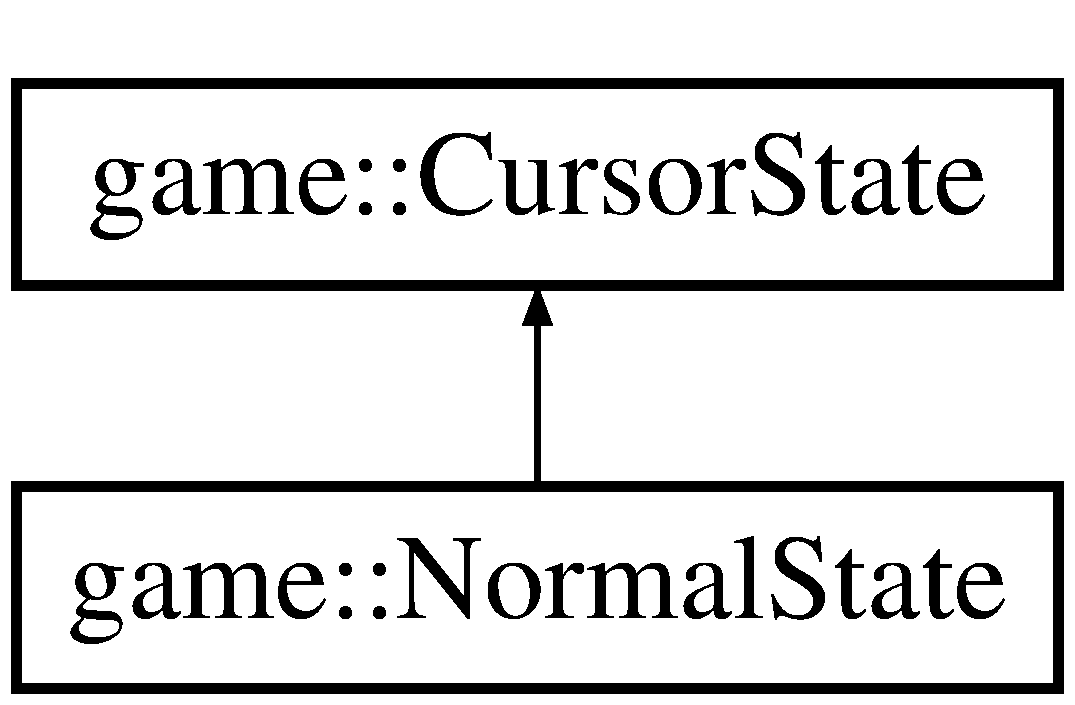
\includegraphics[height=2.000000cm]{classgame_1_1NormalState}
\end{center}
\end{figure}
\subsection*{Public Member Functions}
\begin{DoxyCompactItemize}
\item 
\mbox{\Hypertarget{classgame_1_1NormalState_aa62668ebf4796000df8d0ac13881059a}\label{classgame_1_1NormalState_aa62668ebf4796000df8d0ac13881059a}} 
{\bfseries Normal\+State} (\hyperlink{classgame_1_1Cursor}{Cursor} $\ast$c, \hyperlink{classgame_1_1GameDialog}{Game\+Dialog} $\ast$g\+Dialog)
\item 
\mbox{\Hypertarget{classgame_1_1NormalState_aab1f97ad9dbdbd2a22a777ac2008292b}\label{classgame_1_1NormalState_aab1f97ad9dbdbd2a22a777ac2008292b}} 
void {\bfseries process\+Mouse\+Event} (Q\+Mouse\+Event $\ast$event)
\item 
\mbox{\Hypertarget{classgame_1_1NormalState_ae4409bfac9558b3b9a70ca8be8f9ecb9}\label{classgame_1_1NormalState_ae4409bfac9558b3b9a70ca8be8f9ecb9}} 
void {\bfseries process\+Mouse\+Press} (Q\+Mouse\+Event $\ast$event)
\item 
\mbox{\Hypertarget{classgame_1_1NormalState_a8efa205e3ae635b2cf302e03e85ada2d}\label{classgame_1_1NormalState_a8efa205e3ae635b2cf302e03e85ada2d}} 
void {\bfseries process\+Mouse\+Release} (Q\+Mouse\+Event $\ast$event)
\item 
\mbox{\Hypertarget{classgame_1_1NormalState_a2aa40d550877101c1a0ceaf66a989c94}\label{classgame_1_1NormalState_a2aa40d550877101c1a0ceaf66a989c94}} 
void {\bfseries update\+Cursor\+Display} ()
\item 
\mbox{\Hypertarget{classgame_1_1NormalState_aeeeac9fc5333b16f8b99fa0b3b78be3d}\label{classgame_1_1NormalState_aeeeac9fc5333b16f8b99fa0b3b78be3d}} 
void {\bfseries draw} (Q\+Painter $\ast$p)
\item 
\mbox{\Hypertarget{classgame_1_1NormalState_a98dad4f3e4a58fd019b12b103ad6a749}\label{classgame_1_1NormalState_a98dad4f3e4a58fd019b12b103ad6a749}} 
void {\bfseries update} ()
\end{DoxyCompactItemize}
\subsection*{Additional Inherited Members}


The documentation for this class was generated from the following files\+:\begin{DoxyCompactItemize}
\item 
normalstate.\+h\item 
normalstate.\+cpp\end{DoxyCompactItemize}

\hypertarget{classgame_1_1PenState}{}\section{game\+:\+:Pen\+State Class Reference}
\label{classgame_1_1PenState}\index{game\+::\+Pen\+State@{game\+::\+Pen\+State}}
Inheritance diagram for game\+:\+:Pen\+State\+:\begin{figure}[H]
\begin{center}
\leavevmode
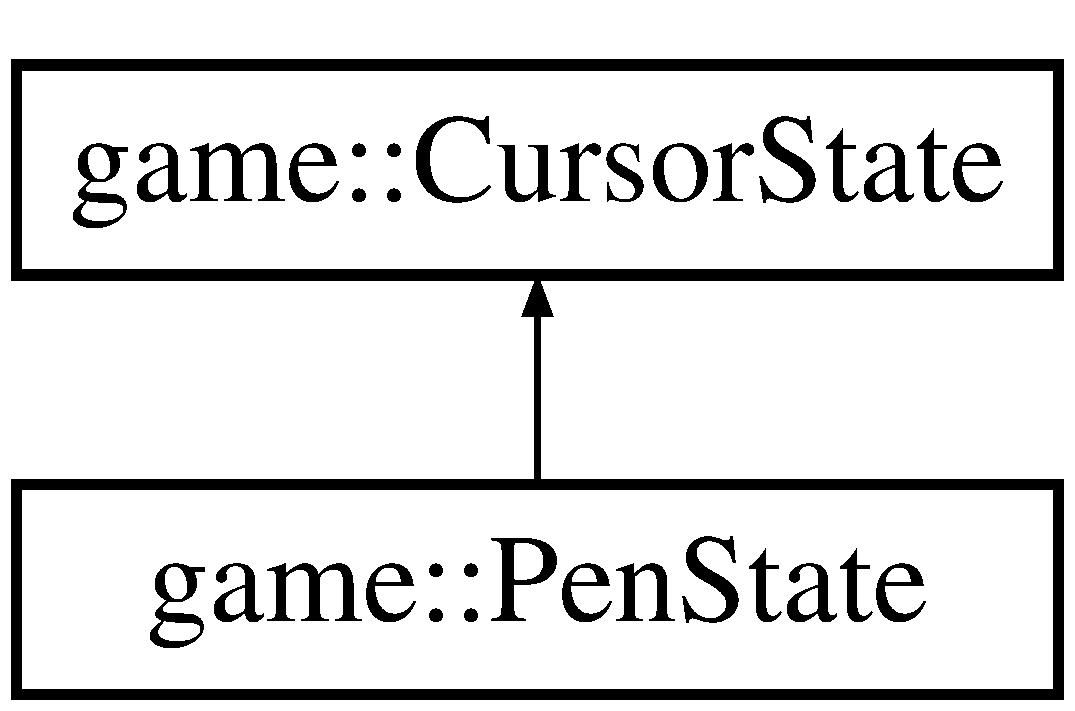
\includegraphics[height=2.000000cm]{classgame_1_1PenState}
\end{center}
\end{figure}
\subsection*{Public Member Functions}
\begin{DoxyCompactItemize}
\item 
\mbox{\Hypertarget{classgame_1_1PenState_a88768f37766e3c41bb8ba20b43a98f1a}\label{classgame_1_1PenState_a88768f37766e3c41bb8ba20b43a98f1a}} 
{\bfseries Pen\+State} (\hyperlink{classgame_1_1Cursor}{Cursor} $\ast$c, \hyperlink{classgame_1_1GameDialog}{Game\+Dialog} $\ast$g\+Dialog)
\item 
\mbox{\Hypertarget{classgame_1_1PenState_ac3587783b7969de4cde8aab83c2409b1}\label{classgame_1_1PenState_ac3587783b7969de4cde8aab83c2409b1}} 
void {\bfseries process\+Mouse\+Event} (Q\+Mouse\+Event $\ast$event)
\item 
\mbox{\Hypertarget{classgame_1_1PenState_a65cdd687ea21c668bd38a519d42d4645}\label{classgame_1_1PenState_a65cdd687ea21c668bd38a519d42d4645}} 
void {\bfseries process\+Mouse\+Press} (Q\+Mouse\+Event $\ast$event)
\item 
\mbox{\Hypertarget{classgame_1_1PenState_abaa4c65c5bf2e5c6a971846505404b19}\label{classgame_1_1PenState_abaa4c65c5bf2e5c6a971846505404b19}} 
void {\bfseries process\+Mouse\+Release} (Q\+Mouse\+Event $\ast$event)
\item 
\mbox{\Hypertarget{classgame_1_1PenState_a6e75396e7a3836cc29346e053e12f043}\label{classgame_1_1PenState_a6e75396e7a3836cc29346e053e12f043}} 
void {\bfseries update\+Cursor\+Display} ()
\item 
\mbox{\Hypertarget{classgame_1_1PenState_af6ec931870dc6e85e8155e3a88397f4d}\label{classgame_1_1PenState_af6ec931870dc6e85e8155e3a88397f4d}} 
void {\bfseries draw} (Q\+Painter $\ast$p)
\item 
\mbox{\Hypertarget{classgame_1_1PenState_a87b7c52a9c47d4024352d21365eb063a}\label{classgame_1_1PenState_a87b7c52a9c47d4024352d21365eb063a}} 
void {\bfseries update} ()
\end{DoxyCompactItemize}
\subsection*{Additional Inherited Members}


The documentation for this class was generated from the following files\+:\begin{DoxyCompactItemize}
\item 
penstate.\+h\item 
penstate.\+cpp\end{DoxyCompactItemize}

\hypertarget{classgame_1_1Powerup}{}\section{game\+:\+:Powerup Class Reference}
\label{classgame_1_1Powerup}\index{game\+::\+Powerup@{game\+::\+Powerup}}
\subsection*{Public Member Functions}
\begin{DoxyCompactItemize}
\item 
\mbox{\Hypertarget{classgame_1_1Powerup_aa307799b1506bc5912c326d3a4b9aa6e}\label{classgame_1_1Powerup_aa307799b1506bc5912c326d3a4b9aa6e}} 
{\bfseries Powerup} (Powerup\+Type type, int x, int y, int radius)
\item 
\mbox{\Hypertarget{classgame_1_1Powerup_a57020b9b245c52bbae1e6f947b4fa8d0}\label{classgame_1_1Powerup_a57020b9b245c52bbae1e6f947b4fa8d0}} 
void {\bfseries draw} (Q\+Painter $\ast$p)
\item 
\mbox{\Hypertarget{classgame_1_1Powerup_a6f53498b83a28f80d50ab4b588b6933a}\label{classgame_1_1Powerup_a6f53498b83a28f80d50ab4b588b6933a}} 
void {\bfseries update} ()
\item 
\mbox{\Hypertarget{classgame_1_1Powerup_a27030babd43cd3e8701a9b8c44b02ecf}\label{classgame_1_1Powerup_a27030babd43cd3e8701a9b8c44b02ecf}} 
int {\bfseries x} ()
\item 
\mbox{\Hypertarget{classgame_1_1Powerup_ada6307d0b7f556d31eb7f7052dacd4f3}\label{classgame_1_1Powerup_ada6307d0b7f556d31eb7f7052dacd4f3}} 
int {\bfseries y} ()
\end{DoxyCompactItemize}
\subsection*{Static Public Member Functions}
\begin{DoxyCompactItemize}
\item 
\mbox{\Hypertarget{classgame_1_1Powerup_afb95079f35c447eb5cc1a896dc307589}\label{classgame_1_1Powerup_afb95079f35c447eb5cc1a896dc307589}} 
static \hyperlink{classgame_1_1Powerup}{Powerup} {\bfseries generate\+Random\+Powerup} (int x, int y, int radius)
\end{DoxyCompactItemize}
\subsection*{Public Attributes}
\begin{DoxyCompactItemize}
\item 
\mbox{\Hypertarget{classgame_1_1Powerup_ab412d4b3a4ca7d9943b93ae7c66fb9c9}\label{classgame_1_1Powerup_ab412d4b3a4ca7d9943b93ae7c66fb9c9}} 
int {\bfseries radius}
\item 
\mbox{\Hypertarget{classgame_1_1Powerup_a31242c7e6021b637ce6a764f6b1baa74}\label{classgame_1_1Powerup_a31242c7e6021b637ce6a764f6b1baa74}} 
Powerup\+Type {\bfseries type}
\item 
\mbox{\Hypertarget{classgame_1_1Powerup_aa2c7842a03a4a3d1efa31cbf63a2d530}\label{classgame_1_1Powerup_aa2c7842a03a4a3d1efa31cbf63a2d530}} 
Q\+Pixmap {\bfseries pixmap}
\end{DoxyCompactItemize}


The documentation for this class was generated from the following files\+:\begin{DoxyCompactItemize}
\item 
powerup.\+h\item 
powerup.\+cpp\end{DoxyCompactItemize}

\hypertarget{classgame_1_1Ship}{}\section{game\+:\+:Ship Class Reference}
\label{classgame_1_1Ship}\index{game\+::\+Ship@{game\+::\+Ship}}
Inheritance diagram for game\+:\+:Ship\+:\begin{figure}[H]
\begin{center}
\leavevmode
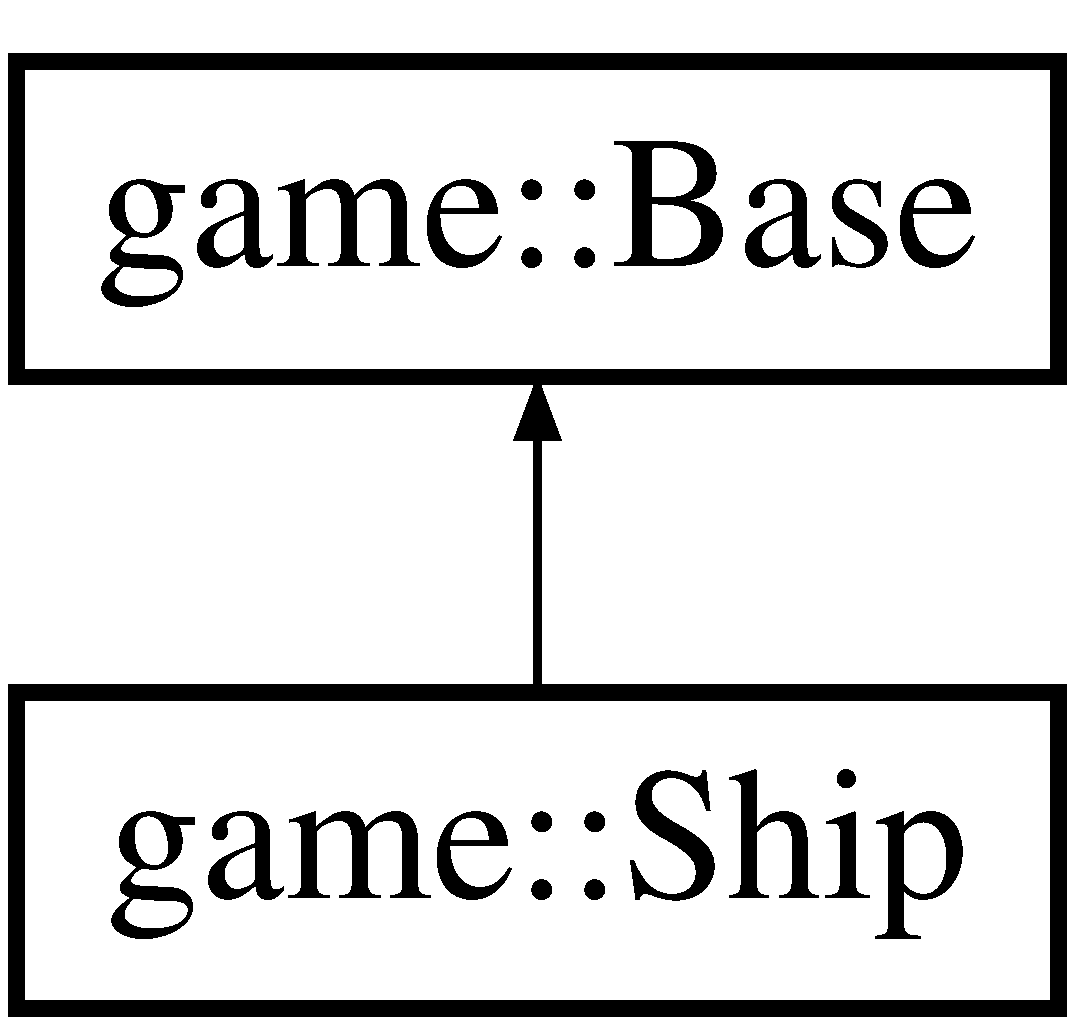
\includegraphics[height=2.000000cm]{classgame_1_1Ship}
\end{center}
\end{figure}
\subsection*{Public Member Functions}
\begin{DoxyCompactItemize}
\item 
\mbox{\Hypertarget{classgame_1_1Ship_a3231025c60af120a20baa522b1c0df74}\label{classgame_1_1Ship_a3231025c60af120a20baa522b1c0df74}} 
{\bfseries Ship} (Q\+Pixmap image, double scale, int x, int y)
\item 
\mbox{\Hypertarget{classgame_1_1Ship_aaa41bdf4597826fd34508f1adaabebfb}\label{classgame_1_1Ship_aaa41bdf4597826fd34508f1adaabebfb}} 
\hyperlink{classgame_1_1Bullet}{Bullet} $\ast$ {\bfseries shoot} ()
\item 
\mbox{\Hypertarget{classgame_1_1Ship_ad736447878332280237bb94e92196132}\label{classgame_1_1Ship_ad736447878332280237bb94e92196132}} 
void {\bfseries move\+\_\+left} ()
\item 
\mbox{\Hypertarget{classgame_1_1Ship_a139ad86e66b369dc9da2f7081f3205fb}\label{classgame_1_1Ship_a139ad86e66b369dc9da2f7081f3205fb}} 
void {\bfseries move\+\_\+right} ()
\item 
\mbox{\Hypertarget{classgame_1_1Ship_a35750fbe941502979040bddaaef24c7f}\label{classgame_1_1Ship_a35750fbe941502979040bddaaef24c7f}} 
void {\bfseries update} ()
\end{DoxyCompactItemize}
\subsection*{Public Attributes}
\begin{DoxyCompactItemize}
\item 
\mbox{\Hypertarget{classgame_1_1Ship_a43e9dadec1741f046cfac0522386da0d}\label{classgame_1_1Ship_a43e9dadec1741f046cfac0522386da0d}} 
bool {\bfseries dead}
\item 
\mbox{\Hypertarget{classgame_1_1Ship_a70b25ad47b9e9a65ab2f6c34c4ce3174}\label{classgame_1_1Ship_a70b25ad47b9e9a65ab2f6c34c4ce3174}} 
Cannon\+Type {\bfseries cannon\+Type}
\item 
\mbox{\Hypertarget{classgame_1_1Ship_a397681e2c3a543a411a8d5addc6bf2b1}\label{classgame_1_1Ship_a397681e2c3a543a411a8d5addc6bf2b1}} 
int {\bfseries cannon\+Ammo}
\item 
\mbox{\Hypertarget{classgame_1_1Ship_aaad695df6b0fb0b9187df5da1d0475a6}\label{classgame_1_1Ship_aaad695df6b0fb0b9187df5da1d0475a6}} 
bool {\bfseries machine\+Gun\+Shoot\+At\+Left}
\end{DoxyCompactItemize}
\subsection*{Additional Inherited Members}


The documentation for this class was generated from the following files\+:\begin{DoxyCompactItemize}
\item 
ship.\+h\item 
ship.\+cpp\end{DoxyCompactItemize}

\hypertarget{structgame_1_1SMakerPlacedObject}{}\section{game\+:\+:S\+Maker\+Placed\+Object Struct Reference}
\label{structgame_1_1SMakerPlacedObject}\index{game\+::\+S\+Maker\+Placed\+Object@{game\+::\+S\+Maker\+Placed\+Object}}
\subsection*{Public Attributes}
\begin{DoxyCompactItemize}
\item 
\mbox{\Hypertarget{structgame_1_1SMakerPlacedObject_a0e5abd288aee052079c1b7c6be43a41a}\label{structgame_1_1SMakerPlacedObject_a0e5abd288aee052079c1b7c6be43a41a}} 
Q\+Rect {\bfseries hit\+Box}
\item 
\mbox{\Hypertarget{structgame_1_1SMakerPlacedObject_a26c241e7e27c53141fe94d6e3f0ce427}\label{structgame_1_1SMakerPlacedObject_a26c241e7e27c53141fe94d6e3f0ce427}} 
S\+Maker\+Object\+Type {\bfseries type}
\item 
\mbox{\Hypertarget{structgame_1_1SMakerPlacedObject_aac05c41b7e6ceee2918b5768425df092}\label{structgame_1_1SMakerPlacedObject_aac05c41b7e6ceee2918b5768425df092}} 
Q\+Pixmap {\bfseries pixmap}
\item 
\mbox{\Hypertarget{structgame_1_1SMakerPlacedObject_a48ae9cd156af2a331caeda4cd0883564}\label{structgame_1_1SMakerPlacedObject_a48ae9cd156af2a331caeda4cd0883564}} 
bool {\bfseries connected}
\item 
\mbox{\Hypertarget{structgame_1_1SMakerPlacedObject_a2cf5fc2086cd06e75beabe8369f4eb52}\label{structgame_1_1SMakerPlacedObject_a2cf5fc2086cd06e75beabe8369f4eb52}} 
Q\+Point {\bfseries connected\+Point}
\item 
\mbox{\Hypertarget{structgame_1_1SMakerPlacedObject_a6f0f44d4b86e6fc7ffcf50ed46d04d13}\label{structgame_1_1SMakerPlacedObject_a6f0f44d4b86e6fc7ffcf50ed46d04d13}} 
Q\+String {\bfseries instructions}
\end{DoxyCompactItemize}


The documentation for this struct was generated from the following file\+:\begin{DoxyCompactItemize}
\item 
stagemaker.\+h\end{DoxyCompactItemize}

\hypertarget{classgame_1_1StageMaker}{}\section{game\+:\+:Stage\+Maker Class Reference}
\label{classgame_1_1StageMaker}\index{game\+::\+Stage\+Maker@{game\+::\+Stage\+Maker}}
\subsection*{Public Member Functions}
\begin{DoxyCompactItemize}
\item 
\mbox{\Hypertarget{classgame_1_1StageMaker_af1b6aa7edf5d213a4d3cf5d778f6b495}\label{classgame_1_1StageMaker_af1b6aa7edf5d213a4d3cf5d778f6b495}} 
{\bfseries Stage\+Maker} (\hyperlink{classgame_1_1GameDialog}{Game\+Dialog} $\ast$g\+Dialog)
\item 
\mbox{\Hypertarget{classgame_1_1StageMaker_ad871b4aea521ed921c3f4b06041d1085}\label{classgame_1_1StageMaker_ad871b4aea521ed921c3f4b06041d1085}} 
void {\bfseries init} ()
\item 
\mbox{\Hypertarget{classgame_1_1StageMaker_a84c160105ae30fb7537880a7c4011a86}\label{classgame_1_1StageMaker_a84c160105ae30fb7537880a7c4011a86}} 
void {\bfseries draw} (Q\+Painter $\ast$p)
\item 
\mbox{\Hypertarget{classgame_1_1StageMaker_a6e08f5b6ff467119e3e5f576ab2195b7}\label{classgame_1_1StageMaker_a6e08f5b6ff467119e3e5f576ab2195b7}} 
void {\bfseries update} ()
\item 
\mbox{\Hypertarget{classgame_1_1StageMaker_ab2b138692289443cb436c517783adbe7}\label{classgame_1_1StageMaker_ab2b138692289443cb436c517783adbe7}} 
void {\bfseries button\+Pressed} ()
\item 
\mbox{\Hypertarget{classgame_1_1StageMaker_a1ac9a3b373bc78e1d504ed20347fd190}\label{classgame_1_1StageMaker_a1ac9a3b373bc78e1d504ed20347fd190}} 
void {\bfseries button\+Released} ()
\item 
\mbox{\Hypertarget{classgame_1_1StageMaker_aed57e4d242bce8bc2e57f446122eaea0}\label{classgame_1_1StageMaker_aed57e4d242bce8bc2e57f446122eaea0}} 
void {\bfseries clear\+All} ()
\item 
\mbox{\Hypertarget{classgame_1_1StageMaker_a00bba225c35cac171f2dc2a13a2cad07}\label{classgame_1_1StageMaker_a00bba225c35cac171f2dc2a13a2cad07}} 
void {\bfseries test\+Stage} ()
\end{DoxyCompactItemize}
\subsection*{Public Attributes}
\begin{DoxyCompactItemize}
\item 
\mbox{\Hypertarget{classgame_1_1StageMaker_a3ff6460868ff3cc0439fec9a2c196f5f}\label{classgame_1_1StageMaker_a3ff6460868ff3cc0439fec9a2c196f5f}} 
std\+::map$<$ S\+Maker\+Object\+Type, \hyperlink{structgame_1_1SMakerPlacedObject}{S\+Maker\+Placed\+Object} $>$ {\bfseries object\+Template}
\item 
\mbox{\Hypertarget{classgame_1_1StageMaker_a388399f9012b668f9a04e23589ce0de2}\label{classgame_1_1StageMaker_a388399f9012b668f9a04e23589ce0de2}} 
Q\+Point {\bfseries line\+Origin}
\item 
\mbox{\Hypertarget{classgame_1_1StageMaker_a2274c1b67f7c3b0865c216ce26f89681}\label{classgame_1_1StageMaker_a2274c1b67f7c3b0865c216ce26f89681}} 
Q\+Rect {\bfseries clear\+All\+Btn}
\item 
\mbox{\Hypertarget{classgame_1_1StageMaker_a2f50a43554a07016d24da52303a3a4f8}\label{classgame_1_1StageMaker_a2f50a43554a07016d24da52303a3a4f8}} 
Q\+Rect {\bfseries test\+Stage\+Btn}
\item 
\mbox{\Hypertarget{classgame_1_1StageMaker_a92871f28725f6b66ed40c1a1d91496f8}\label{classgame_1_1StageMaker_a92871f28725f6b66ed40c1a1d91496f8}} 
S\+Maker\+Object\+Type {\bfseries holding\+Object}
\item 
\mbox{\Hypertarget{classgame_1_1StageMaker_ab8ac20dea0d9f79f56c2b1b6ab225fa7}\label{classgame_1_1StageMaker_ab8ac20dea0d9f79f56c2b1b6ab225fa7}} 
\hyperlink{classgame_1_1GameDialog}{Game\+Dialog} $\ast$ {\bfseries g\+Dialog}
\end{DoxyCompactItemize}


The documentation for this class was generated from the following files\+:\begin{DoxyCompactItemize}
\item 
stagemaker.\+h\item 
stagemaker.\+cpp\end{DoxyCompactItemize}

\hypertarget{structstar}{}\section{star Struct Reference}
\label{structstar}\index{star@{star}}
\subsection*{Public Attributes}
\begin{DoxyCompactItemize}
\item 
\mbox{\Hypertarget{structstar_ae7e9935c7a2052ec9f292c6a95ad16dc}\label{structstar_ae7e9935c7a2052ec9f292c6a95ad16dc}} 
int {\bfseries x}
\item 
\mbox{\Hypertarget{structstar_a5532234288af217e0113dcc1ab7f1072}\label{structstar_a5532234288af217e0113dcc1ab7f1072}} 
int {\bfseries y}
\item 
\mbox{\Hypertarget{structstar_af34562c391e08523e96e2ea2ca16f60d}\label{structstar_af34562c391e08523e96e2ea2ca16f60d}} 
Q\+Color {\bfseries color}
\item 
\mbox{\Hypertarget{structstar_a684efdbc7fa0ea5230e760f0881ae5ca}\label{structstar_a684efdbc7fa0ea5230e760f0881ae5ca}} 
int {\bfseries speed}
\end{DoxyCompactItemize}


The documentation for this struct was generated from the following file\+:\begin{DoxyCompactItemize}
\item 
background.\+h\end{DoxyCompactItemize}

\hypertarget{classgame_1_1StatusBar}{}\section{game\+:\+:Status\+Bar Class Reference}
\label{classgame_1_1StatusBar}\index{game\+::\+Status\+Bar@{game\+::\+Status\+Bar}}
\subsection*{Public Member Functions}
\begin{DoxyCompactItemize}
\item 
\mbox{\Hypertarget{classgame_1_1StatusBar_aa221673b8c844eed90b156966622f7aa}\label{classgame_1_1StatusBar_aa221673b8c844eed90b156966622f7aa}} 
{\bfseries Status\+Bar} (\hyperlink{classgame_1_1GameDialog}{Game\+Dialog} $\ast$dialog)
\item 
\mbox{\Hypertarget{classgame_1_1StatusBar_a07da42cf14cef3b91fbacb08babeba57}\label{classgame_1_1StatusBar_a07da42cf14cef3b91fbacb08babeba57}} 
void {\bfseries draw} (Q\+Painter $\ast$p)
\item 
\mbox{\Hypertarget{classgame_1_1StatusBar_ac10ba09b74a617b029fc85e3e806d9df}\label{classgame_1_1StatusBar_ac10ba09b74a617b029fc85e3e806d9df}} 
void {\bfseries update} ()
\item 
\mbox{\Hypertarget{classgame_1_1StatusBar_a1e35813d42009779f3c24f7ac7ac6fe6}\label{classgame_1_1StatusBar_a1e35813d42009779f3c24f7ac7ac6fe6}} 
void {\bfseries build\+Brush} ()
\end{DoxyCompactItemize}
\subsection*{Public Attributes}
\begin{DoxyCompactItemize}
\item 
\mbox{\Hypertarget{classgame_1_1StatusBar_a7f689a9d2af31928c419676f7eb7574d}\label{classgame_1_1StatusBar_a7f689a9d2af31928c419676f7eb7574d}} 
double {\bfseries plasma\+Energy}
\item 
\mbox{\Hypertarget{classgame_1_1StatusBar_a163659b0b66f80294b8e14630fa61f92}\label{classgame_1_1StatusBar_a163659b0b66f80294b8e14630fa61f92}} 
double {\bfseries barrier\+Energy}
\item 
\mbox{\Hypertarget{classgame_1_1StatusBar_af653577a3a51facb48406cc4d8be1bf7}\label{classgame_1_1StatusBar_af653577a3a51facb48406cc4d8be1bf7}} 
\hyperlink{classgame_1_1GameDialog}{Game\+Dialog} $\ast$ {\bfseries gd}
\item 
\mbox{\Hypertarget{classgame_1_1StatusBar_aff1f3af82e8cc7acab25a2dcd138bc12}\label{classgame_1_1StatusBar_aff1f3af82e8cc7acab25a2dcd138bc12}} 
Q\+Rect {\bfseries container\+Outer}
\item 
\mbox{\Hypertarget{classgame_1_1StatusBar_a6aac9db1ee5c17fa560029c44bafef2f}\label{classgame_1_1StatusBar_a6aac9db1ee5c17fa560029c44bafef2f}} 
Q\+Rect {\bfseries container\+Inner}
\item 
\mbox{\Hypertarget{classgame_1_1StatusBar_a913f4b61e040916ecc74b860ea6aae93}\label{classgame_1_1StatusBar_a913f4b61e040916ecc74b860ea6aae93}} 
Q\+Rect {\bfseries status\+Bar}
\item 
\mbox{\Hypertarget{classgame_1_1StatusBar_a85e71cdf7723a28c0a074b8e175ec1be}\label{classgame_1_1StatusBar_a85e71cdf7723a28c0a074b8e175ec1be}} 
Q\+Rect {\bfseries plasma\+Bar}
\item 
\mbox{\Hypertarget{classgame_1_1StatusBar_aa8b50fb06a6dd2d6b2dc6aa20bfece17}\label{classgame_1_1StatusBar_aa8b50fb06a6dd2d6b2dc6aa20bfece17}} 
Q\+Rect {\bfseries barrier\+Bar}
\item 
\mbox{\Hypertarget{classgame_1_1StatusBar_a8ca76942546081a6b216750c593a45d5}\label{classgame_1_1StatusBar_a8ca76942546081a6b216750c593a45d5}} 
Q\+Brush {\bfseries status\+Bar\+Brush}
\item 
\mbox{\Hypertarget{classgame_1_1StatusBar_acf54f4d846efa7057076fb2a943fef1d}\label{classgame_1_1StatusBar_acf54f4d846efa7057076fb2a943fef1d}} 
Q\+Brush {\bfseries plasma\+Bar\+Brush}
\item 
\mbox{\Hypertarget{classgame_1_1StatusBar_a477e4348478dad3d4983b520c2184e19}\label{classgame_1_1StatusBar_a477e4348478dad3d4983b520c2184e19}} 
Q\+Brush {\bfseries barrier\+Bar\+Brush}
\item 
\mbox{\Hypertarget{classgame_1_1StatusBar_afc97465ae693e902628a04cc7daf4562}\label{classgame_1_1StatusBar_afc97465ae693e902628a04cc7daf4562}} 
bool {\bfseries plasma\+Drained}
\end{DoxyCompactItemize}


The documentation for this class was generated from the following files\+:\begin{DoxyCompactItemize}
\item 
statusbar.\+h\item 
statusbar.\+cpp\end{DoxyCompactItemize}

\hypertarget{classgame_1_1Swarm}{}\section{game\+:\+:Swarm Class Reference}
\label{classgame_1_1Swarm}\index{game\+::\+Swarm@{game\+::\+Swarm}}
Inheritance diagram for game\+:\+:Swarm\+:\begin{figure}[H]
\begin{center}
\leavevmode
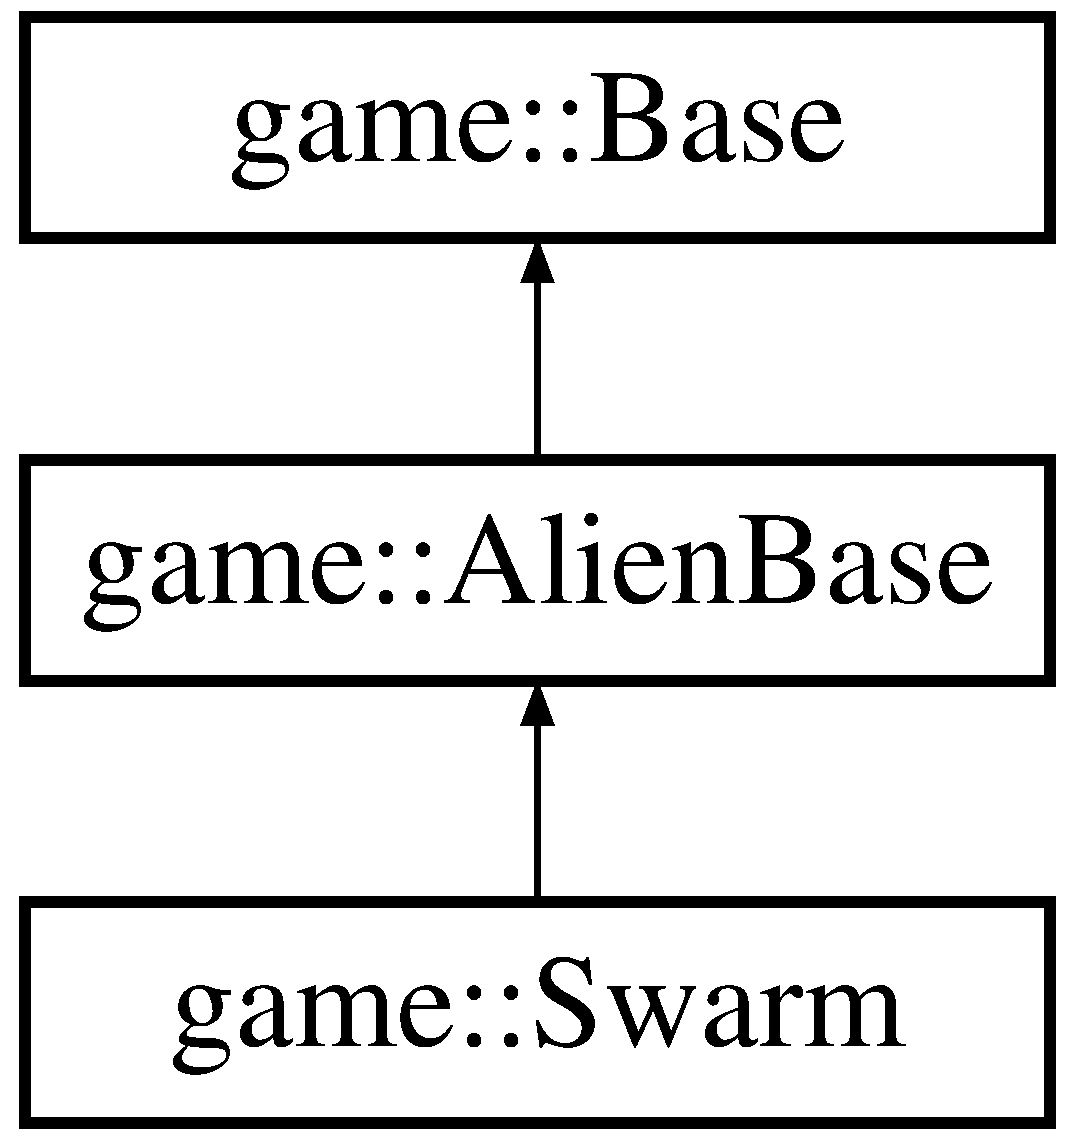
\includegraphics[height=3.000000cm]{classgame_1_1Swarm}
\end{center}
\end{figure}
\subsection*{Public Member Functions}
\begin{DoxyCompactItemize}
\item 
\hyperlink{classgame_1_1Swarm_abb77569228eb93b30ba187991a1c9a6b}{Swarm} (\hyperlink{classgame_1_1SwarmInfo}{Swarm\+Info} \&swarm\+Info, \hyperlink{classgame_1_1Base}{Base} \&ship)
\item 
\mbox{\Hypertarget{classgame_1_1Swarm_a0d4f05f3b4bcdb9bfc339d5017cbb676}\label{classgame_1_1Swarm_a0d4f05f3b4bcdb9bfc339d5017cbb676}} 
bool {\bfseries add} (\hyperlink{classgame_1_1AlienBase}{Alien\+Base} $\ast$to\+Add)
\item 
\mbox{\Hypertarget{classgame_1_1Swarm_a7fd2d1d831a3cee779085727b64b1a28}\label{classgame_1_1Swarm_a7fd2d1d831a3cee779085727b64b1a28}} 
void {\bfseries remove} (\hyperlink{classgame_1_1AlienBase}{Alien\+Base} $\ast$to\+Delete)
\item 
\mbox{\Hypertarget{classgame_1_1Swarm_a658bc4cfff9d0b90b3d78a993122fec5}\label{classgame_1_1Swarm_a658bc4cfff9d0b90b3d78a993122fec5}} 
void {\bfseries move} (Q\+String direction)
\item 
\mbox{\Hypertarget{classgame_1_1Swarm_af4a57a9e2d29d9572a4eecedb8094e88}\label{classgame_1_1Swarm_af4a57a9e2d29d9572a4eecedb8094e88}} 
Q\+List$<$ \hyperlink{classgame_1_1Bullet}{Bullet} $\ast$ $>$ {\bfseries shoot} (Q\+String type)
\item 
\mbox{\Hypertarget{classgame_1_1Swarm_aec4ececc4e0c199ba9e669c20f06099a}\label{classgame_1_1Swarm_aec4ececc4e0c199ba9e669c20f06099a}} 
int {\bfseries get\+\_\+score} () const
\item 
\mbox{\Hypertarget{classgame_1_1Swarm_a4118700e3f584dd12b1157b7706f174b}\label{classgame_1_1Swarm_a4118700e3f584dd12b1157b7706f174b}} 
Q\+List$<$ \hyperlink{classgame_1_1AlienBase}{Alien\+Base} $\ast$ $>$ {\bfseries get\+Aliens} () const
\item 
\mbox{\Hypertarget{classgame_1_1Swarm_a997d0cc9a90667196d8b50ac065f2cf9}\label{classgame_1_1Swarm_a997d0cc9a90667196d8b50ac065f2cf9}} 
Q\+List$<$ \hyperlink{classgame_1_1Bullet}{Bullet} $\ast$ $>$ {\bfseries react} ()
\item 
\mbox{\Hypertarget{classgame_1_1Swarm_ab1b1374558520158868e505ec24547ba}\label{classgame_1_1Swarm_ab1b1374558520158868e505ec24547ba}} 
virtual void {\bfseries paint} (Q\+Painter \&painter)
\end{DoxyCompactItemize}
\subsection*{Additional Inherited Members}


\subsection{Constructor \& Destructor Documentation}
\mbox{\Hypertarget{classgame_1_1Swarm_abb77569228eb93b30ba187991a1c9a6b}\label{classgame_1_1Swarm_abb77569228eb93b30ba187991a1c9a6b}} 
\index{game\+::\+Swarm@{game\+::\+Swarm}!Swarm@{Swarm}}
\index{Swarm@{Swarm}!game\+::\+Swarm@{game\+::\+Swarm}}
\subsubsection{\texorpdfstring{Swarm()}{Swarm()}}
{\footnotesize\ttfamily game\+::\+Swarm\+::\+Swarm (\begin{DoxyParamCaption}\item[{\hyperlink{classgame_1_1SwarmInfo}{Swarm\+Info} \&}]{swarm\+Info,  }\item[{\hyperlink{classgame_1_1Base}{Base} \&}]{ship }\end{DoxyParamCaption})}

C\+O\+N\+S\+T\+R\+U\+C\+T\+OR \begin{quote}
\begin{quote}
\begin{quote}
\begin{quote}
\begin{quote}
\begin{quote}
F\+OR AN E\+M\+P\+TY S\+W\+A\+RM at init (e.\+g., root node) \end{quote}
\end{quote}
\end{quote}
\end{quote}
\end{quote}
\end{quote}
it should A\+L\+W\+A\+YS shoot and move (see max pixels) These following properties for Root swarm nodes are the defaults for swarminfo
\begin{DoxyItemize}
\item moves list is a single \char`\"{}\char`\"{}
\item max\+Pixels should be 0; because everything should always move it should always shoot, if shoot\+Time == 0; just shoot E\+V\+E\+R\+Y\+T\+H\+I\+NG because lower swarms (that are not the root) decide for them selves anyway leaf nodes from the root will always be shooting
\item Image will be some default e.\+g., red\+Invader
\item Type is as above, default is red
\end{DoxyItemize}

\begin{quote}
\begin{quote}
\begin{quote}
\begin{quote}
\begin{quote}
\begin{quote}
Else, just fill out the swarm info and positions\end{quote}
\end{quote}
\end{quote}
\end{quote}
\end{quote}
\end{quote}


The documentation for this class was generated from the following files\+:\begin{DoxyCompactItemize}
\item 
swarm.\+h\item 
swarm.\+cpp\end{DoxyCompactItemize}

\hypertarget{classgame_1_1SwarmInfo}{}\section{game\+:\+:Swarm\+Info Class Reference}
\label{classgame_1_1SwarmInfo}\index{game\+::\+Swarm\+Info@{game\+::\+Swarm\+Info}}
\subsection*{Public Member Functions}
\begin{DoxyCompactItemize}
\item 
\mbox{\Hypertarget{classgame_1_1SwarmInfo_a9409cbebf4b9e4eede6b46dfda8ad893}\label{classgame_1_1SwarmInfo_a9409cbebf4b9e4eede6b46dfda8ad893}} 
{\bfseries Swarm\+Info} (Q\+String type, Q\+List$<$ Q\+Pair$<$ int, int $>$$>$ positions, Q\+String\+List move, int shoot)
\end{DoxyCompactItemize}
\subsection*{Public Attributes}
\begin{DoxyCompactItemize}
\item 
\mbox{\Hypertarget{classgame_1_1SwarmInfo_a8b0dda6f67ca7b7569e01dc9b1b7af7d}\label{classgame_1_1SwarmInfo_a8b0dda6f67ca7b7569e01dc9b1b7af7d}} 
Q\+Pixmap {\bfseries swarm\+Image}
\item 
\mbox{\Hypertarget{classgame_1_1SwarmInfo_a241887ba92116612fb74ec5620877ce4}\label{classgame_1_1SwarmInfo_a241887ba92116612fb74ec5620877ce4}} 
Q\+String {\bfseries type}
\item 
\mbox{\Hypertarget{classgame_1_1SwarmInfo_aad578fbd8c715b8704406c13761e2e02}\label{classgame_1_1SwarmInfo_aad578fbd8c715b8704406c13761e2e02}} 
Q\+List$<$ Q\+Pair$<$ int, int $>$ $>$ {\bfseries positions}
\item 
\mbox{\Hypertarget{classgame_1_1SwarmInfo_aa4eeb90d8e86e13abd7a5a4ed9f7b8ce}\label{classgame_1_1SwarmInfo_aa4eeb90d8e86e13abd7a5a4ed9f7b8ce}} 
Q\+String\+List {\bfseries move}
\item 
\mbox{\Hypertarget{classgame_1_1SwarmInfo_ac5d96ddf1d4e3cedd0d8f3ce0da9fe37}\label{classgame_1_1SwarmInfo_ac5d96ddf1d4e3cedd0d8f3ce0da9fe37}} 
int {\bfseries shoot}
\end{DoxyCompactItemize}


The documentation for this class was generated from the following files\+:\begin{DoxyCompactItemize}
\item 
swarminfo.\+h\item 
swarminfo.\+cpp\end{DoxyCompactItemize}

\hypertarget{classgame_1_1UnitTestSpaceInvader}{}\section{game\+:\+:Unit\+Test\+Space\+Invader Class Reference}
\label{classgame_1_1UnitTestSpaceInvader}\index{game\+::\+Unit\+Test\+Space\+Invader@{game\+::\+Unit\+Test\+Space\+Invader}}
Inheritance diagram for game\+:\+:Unit\+Test\+Space\+Invader\+:\begin{figure}[H]
\begin{center}
\leavevmode
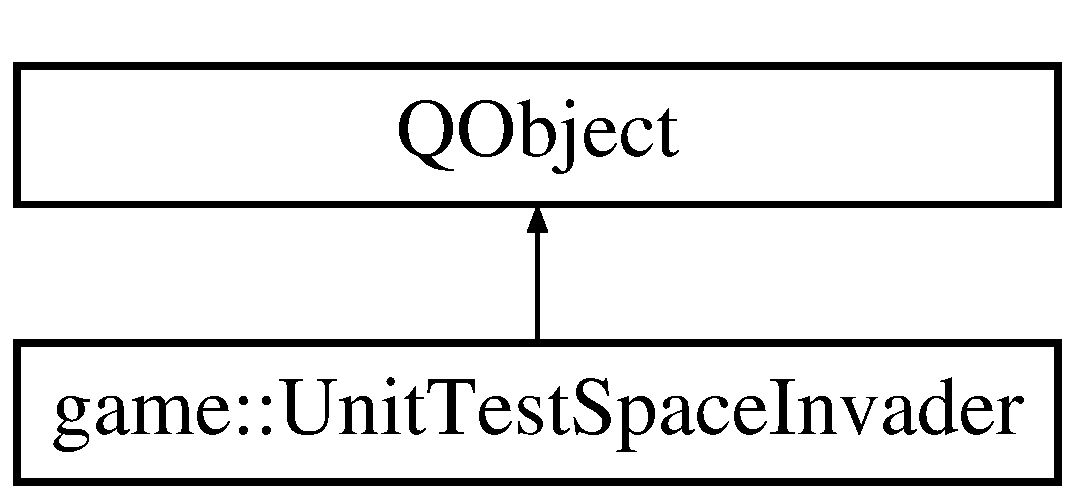
\includegraphics[height=2.000000cm]{classgame_1_1UnitTestSpaceInvader}
\end{center}
\end{figure}


The documentation for this class was generated from the following files\+:\begin{DoxyCompactItemize}
\item 
unittestspaceinvader.\+h\item 
unittestspaceinvader.\+cpp\end{DoxyCompactItemize}

%--- End generated contents ---

% Index
\backmatter
\newpage
\phantomsection
\clearemptydoublepage
\addcontentsline{toc}{chapter}{Index}
\printindex

\end{document}
